% !TEX encoding = UTF-8 Unicode
\documentclass{beamer}

\usepackage{amsmath}
\usepackage{color}
\usepackage{gensymb}
\usepackage{hyperref}
\usepackage{textcomp}
\usepackage{tikz}
\usepackage{verbatim}

\usepackage{listings}
\usepackage{listings}
\lstset{language=Python,
    basicstyle=\ttfamily\bfseries,
    commentstyle=\color{red}\itshape,
    stringstyle=\color{darkolivegreen},
    showstringspaces=false,
    keywordstyle=\color{blue}\bfseries}

\usetheme{Warsaw}

\definecolor{darkolivegreen}{rgb}{0.33, 0.42, 0.18}

\title[ESS 490-590 - AWS tutorial]{Cloud computing: Running your Python code on Amazon Web Services}
\author{Ariane Ducellier}
\institute{University of Washington}
\date{ESS 490-590 Data science for Earth and planetary systems - Spring 2021}

\begin{document}

	\begin{frame}
		\titlepage
	\end{frame}

	\begin{frame}
	\frametitle{First step: Create an AWS Educate account}
	Go to \href{https://aws.amazon.com/education/awseducate/}{https://aws.amazon.com/education/awseducate/}

	\vspace{1cm}

	Creating the account will give you access to AWS tutorials and some AWS credits.
	\end{frame}

	\begin{frame}
	\frametitle{Second step: Create an AWS account}
	Go to \href{https://aws.amazon.com/}{https://aws.amazon.com/}. You will need to enter a credit card number.

	\vspace{1cm}

	Once your account is created, you should be able to redeem your AWS credits.
	\end{frame}

	\begin{frame}
	\frametitle{Most important points}
	\begin{itemize}
		\item Do not forget to terminate your instances.

		\vspace{0.5cm}

		\item Check your billing dashboard on a regular basis.

		\vspace{0.5cm}

		\item The EC2 dashboard shows only instances and keys for the region you have currently selected. Other instances may be running in other regions.
	\end{itemize}
	\end{frame}

	\begin{frame}
	\frametitle{Start working! Open the home page of your AWS account}
	\begin{tikzpicture}
		\node[anchor=south west, inner sep=0] at (0,0) {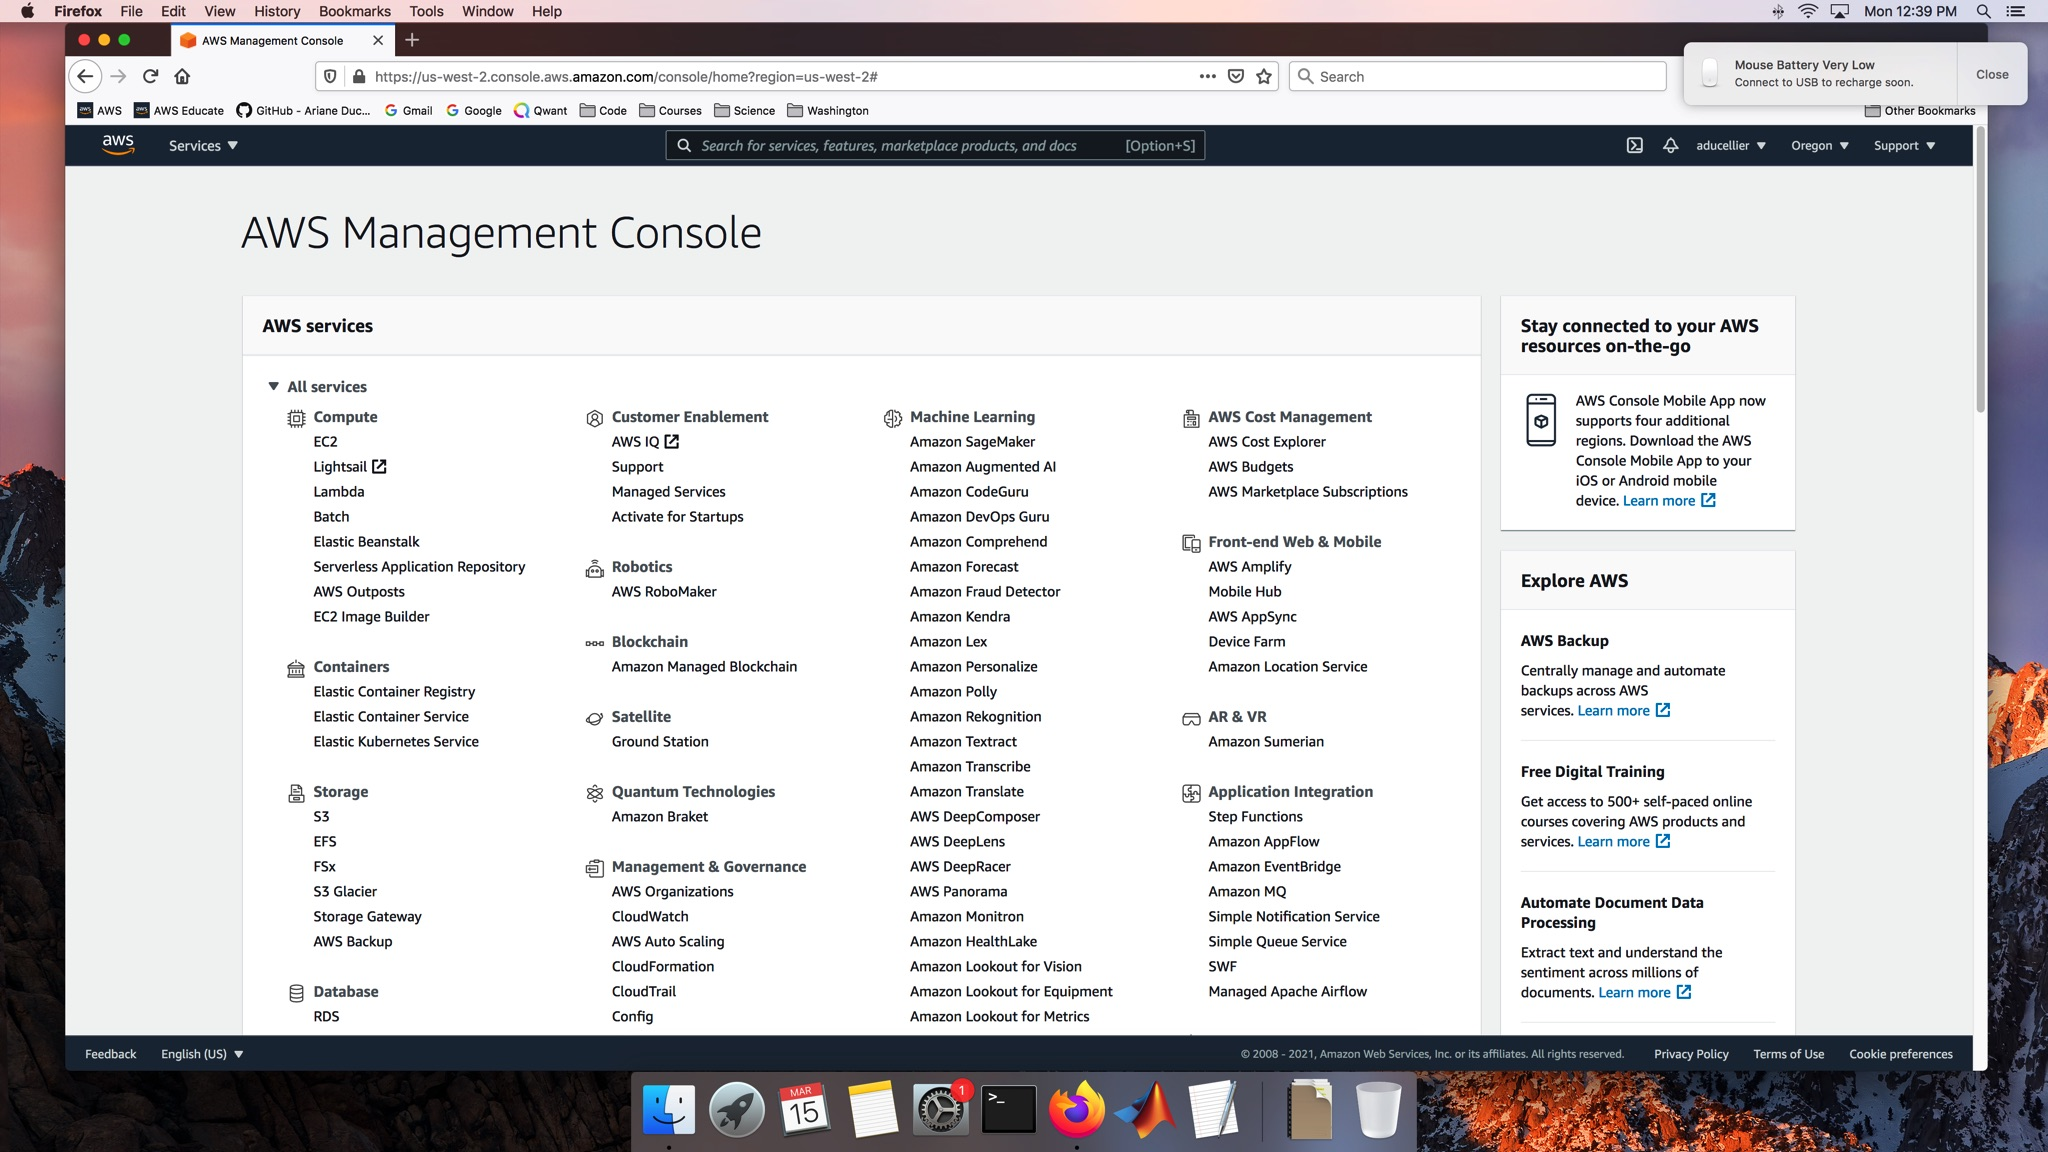
\includegraphics[width=11cm]{figures/AWS_home.jpg}};
		\draw<1>[red, thick] (1.6,3.7) rectangle ++(0.3,0.2);
	\end{tikzpicture}
	\end{frame}

	\begin{frame}
	\frametitle{Check the region where you are (here Oregon = us-west-2)}
	\begin{tikzpicture}
		\node[anchor=south west, inner sep=0] at (0,0) {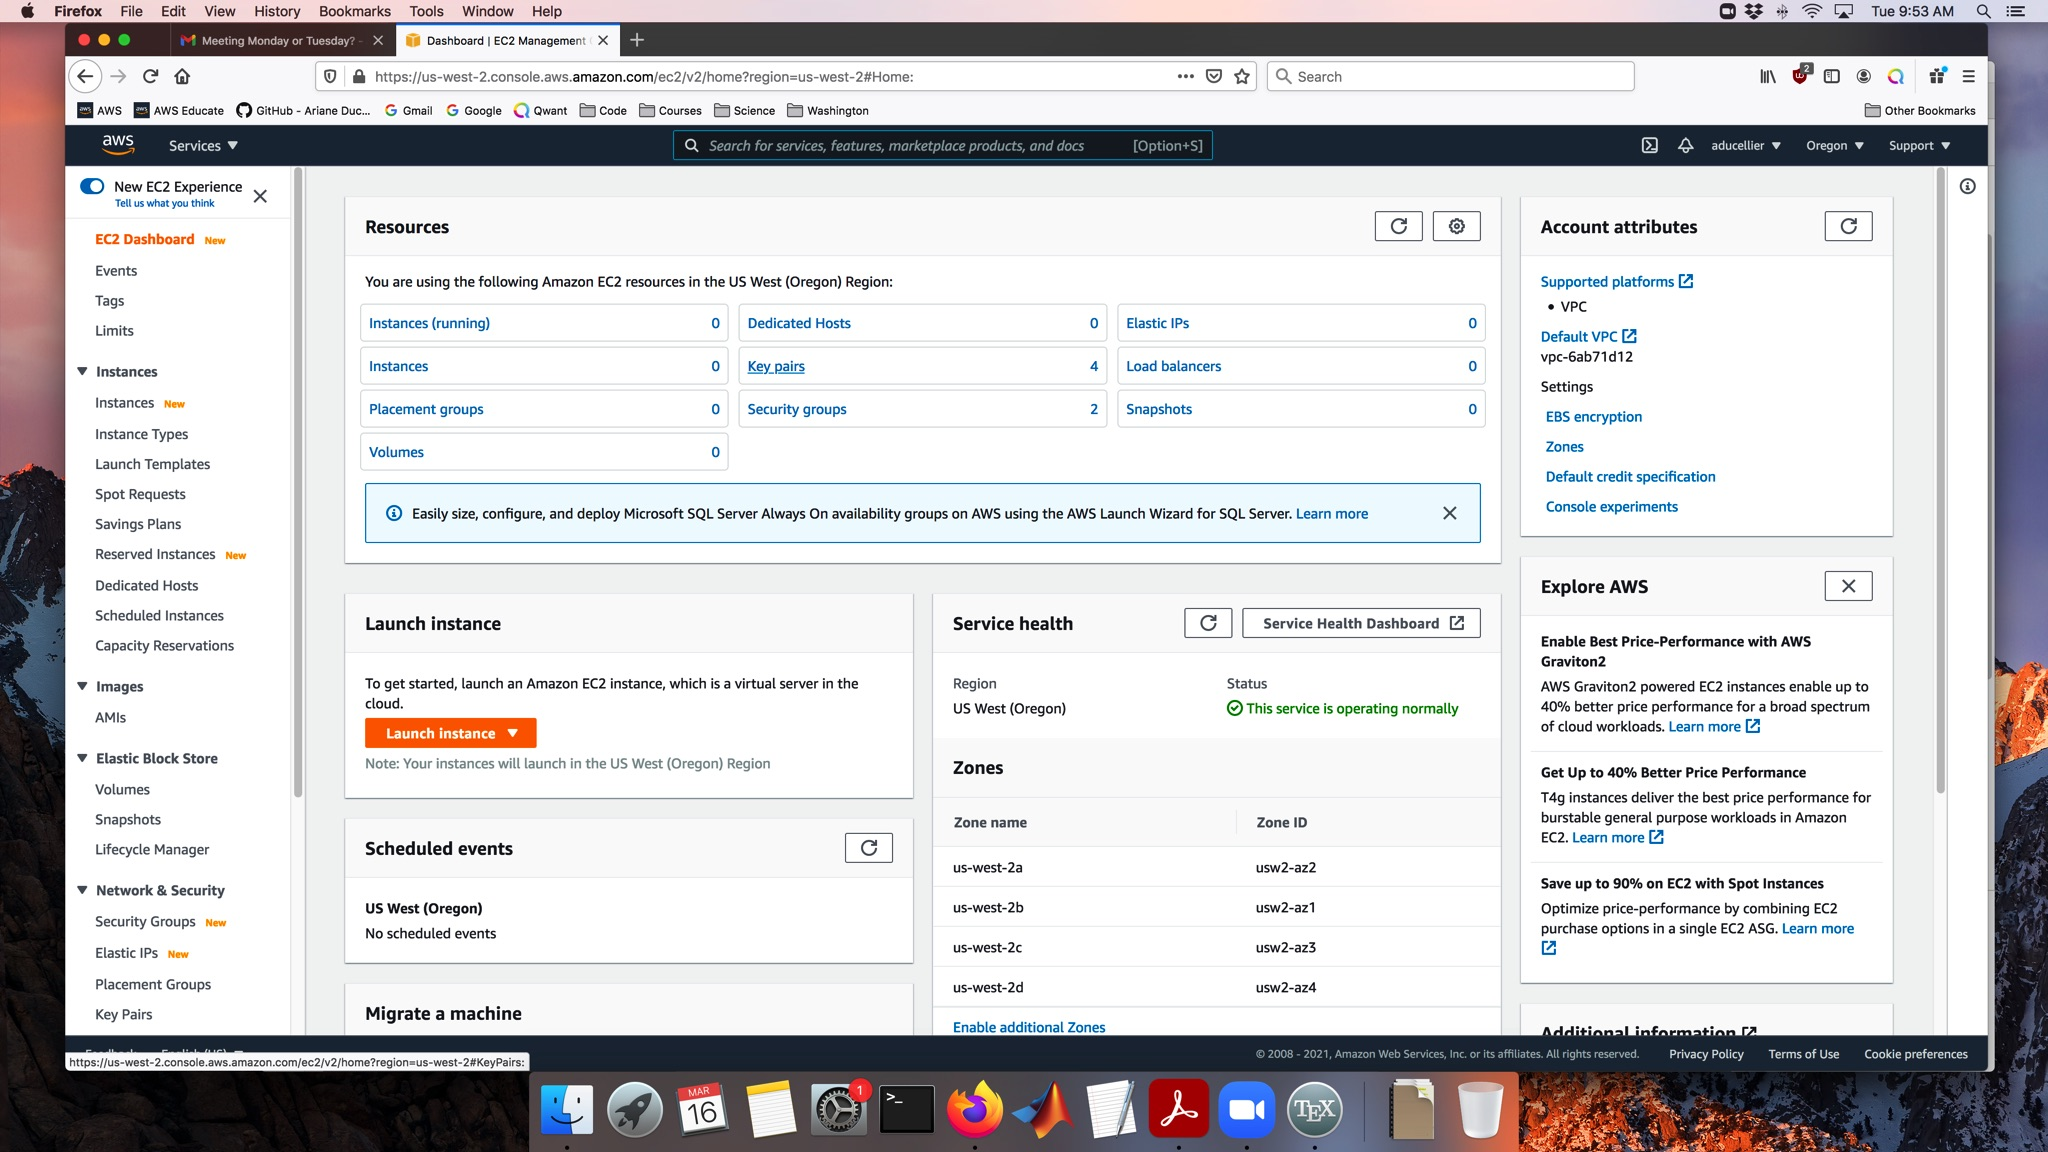
\includegraphics[width=11cm]{figures/EC2_home.jpg}};
		\draw<1>[red, thick] (9.6,5.3) rectangle ++(0.5,0.2);
	\end{tikzpicture}
	\end{frame}

	\begin{frame}
	\frametitle{You need to create a key pair to access EC2 instances}
	\begin{tikzpicture}
		\node[anchor=south west, inner sep=0] at (0,0) {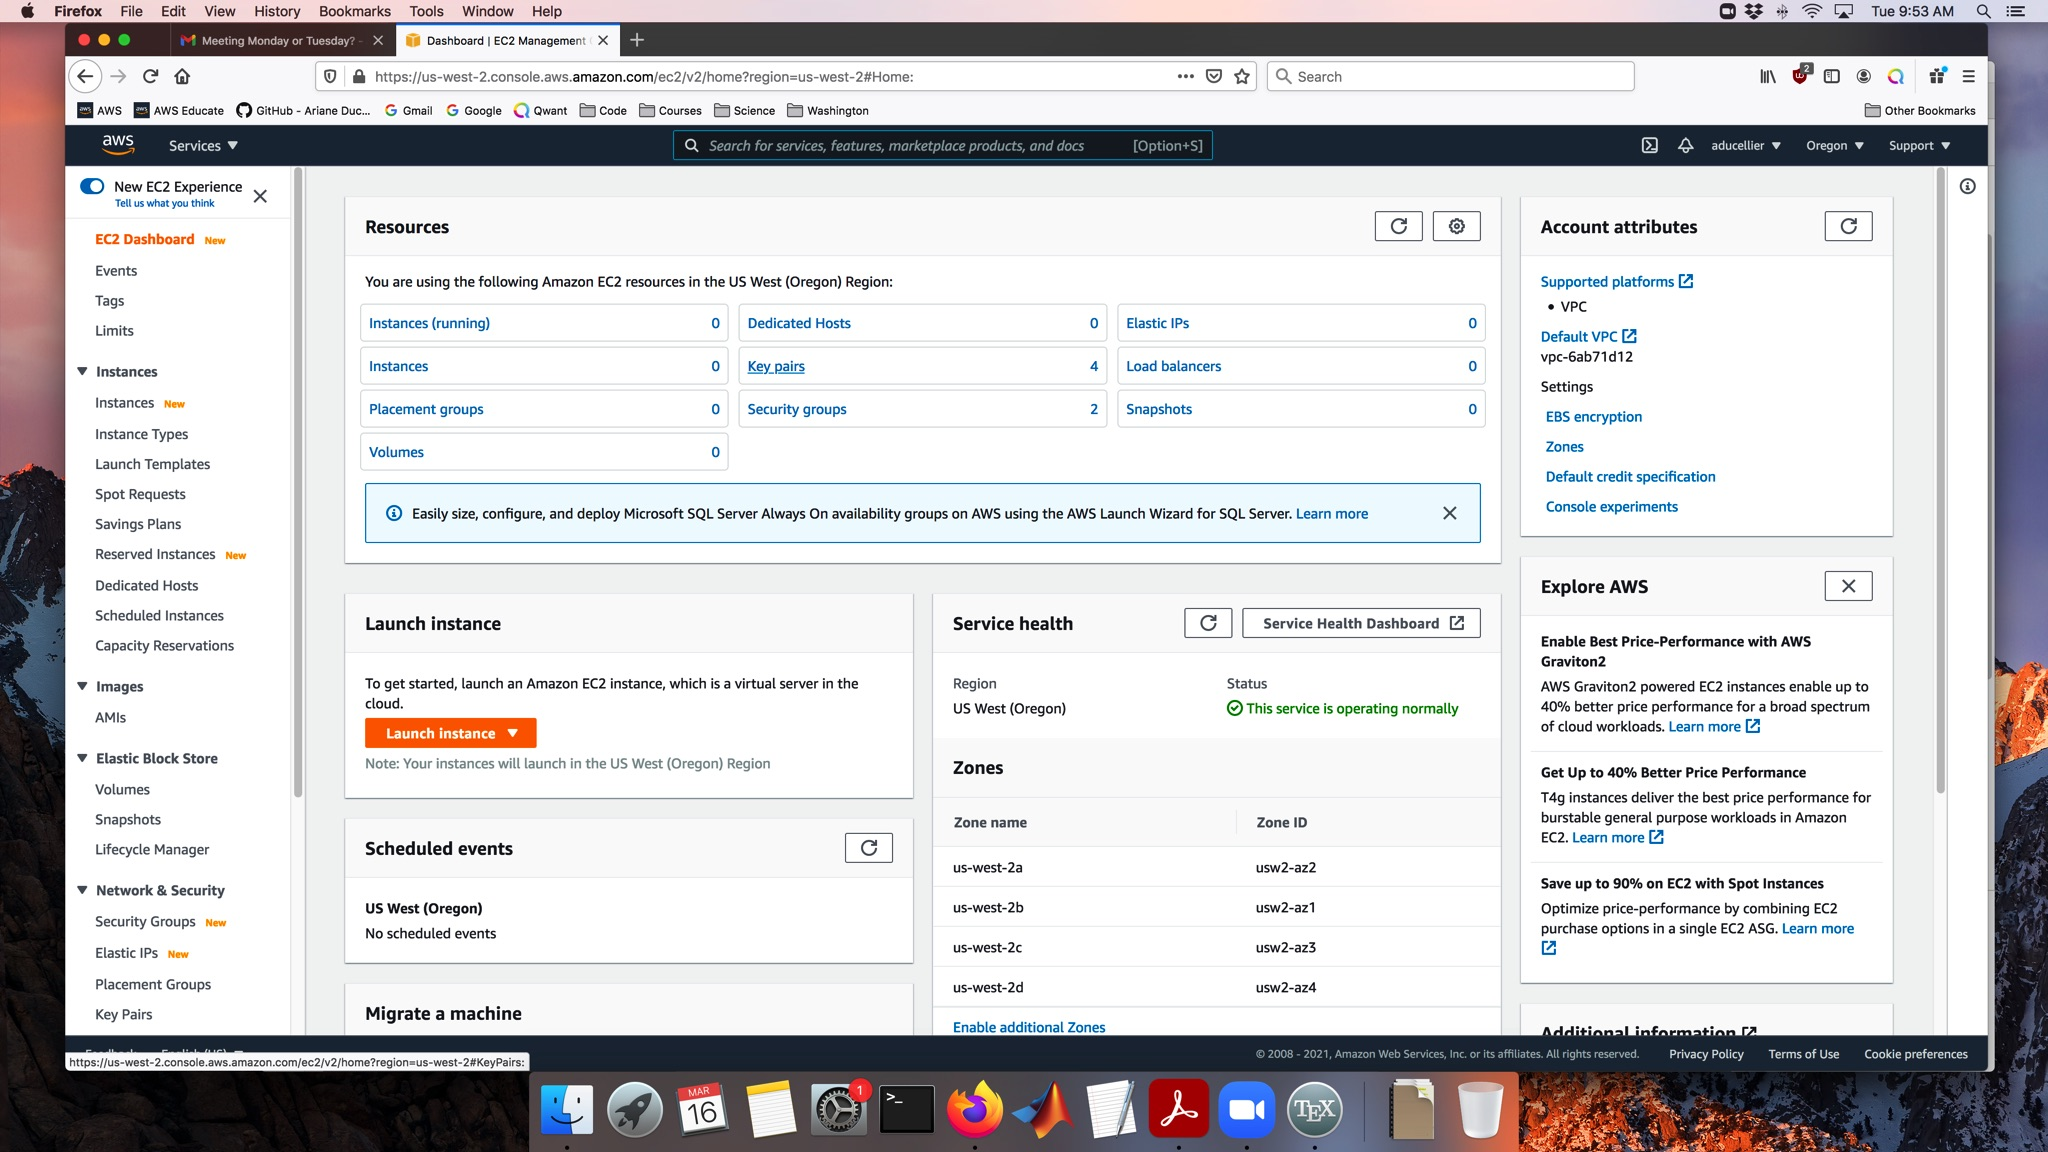
\includegraphics[width=11cm]{figures/EC2_home.jpg}};
		\draw<1>[red, thick] (4,4.1) rectangle ++(0.5,0.2);
	\end{tikzpicture}
	\end{frame}

	\begin{frame}
	\frametitle{Click on \textit{Create key pair} to start}
	\begin{tikzpicture}
		\node[anchor=south west, inner sep=0] at (0,0) {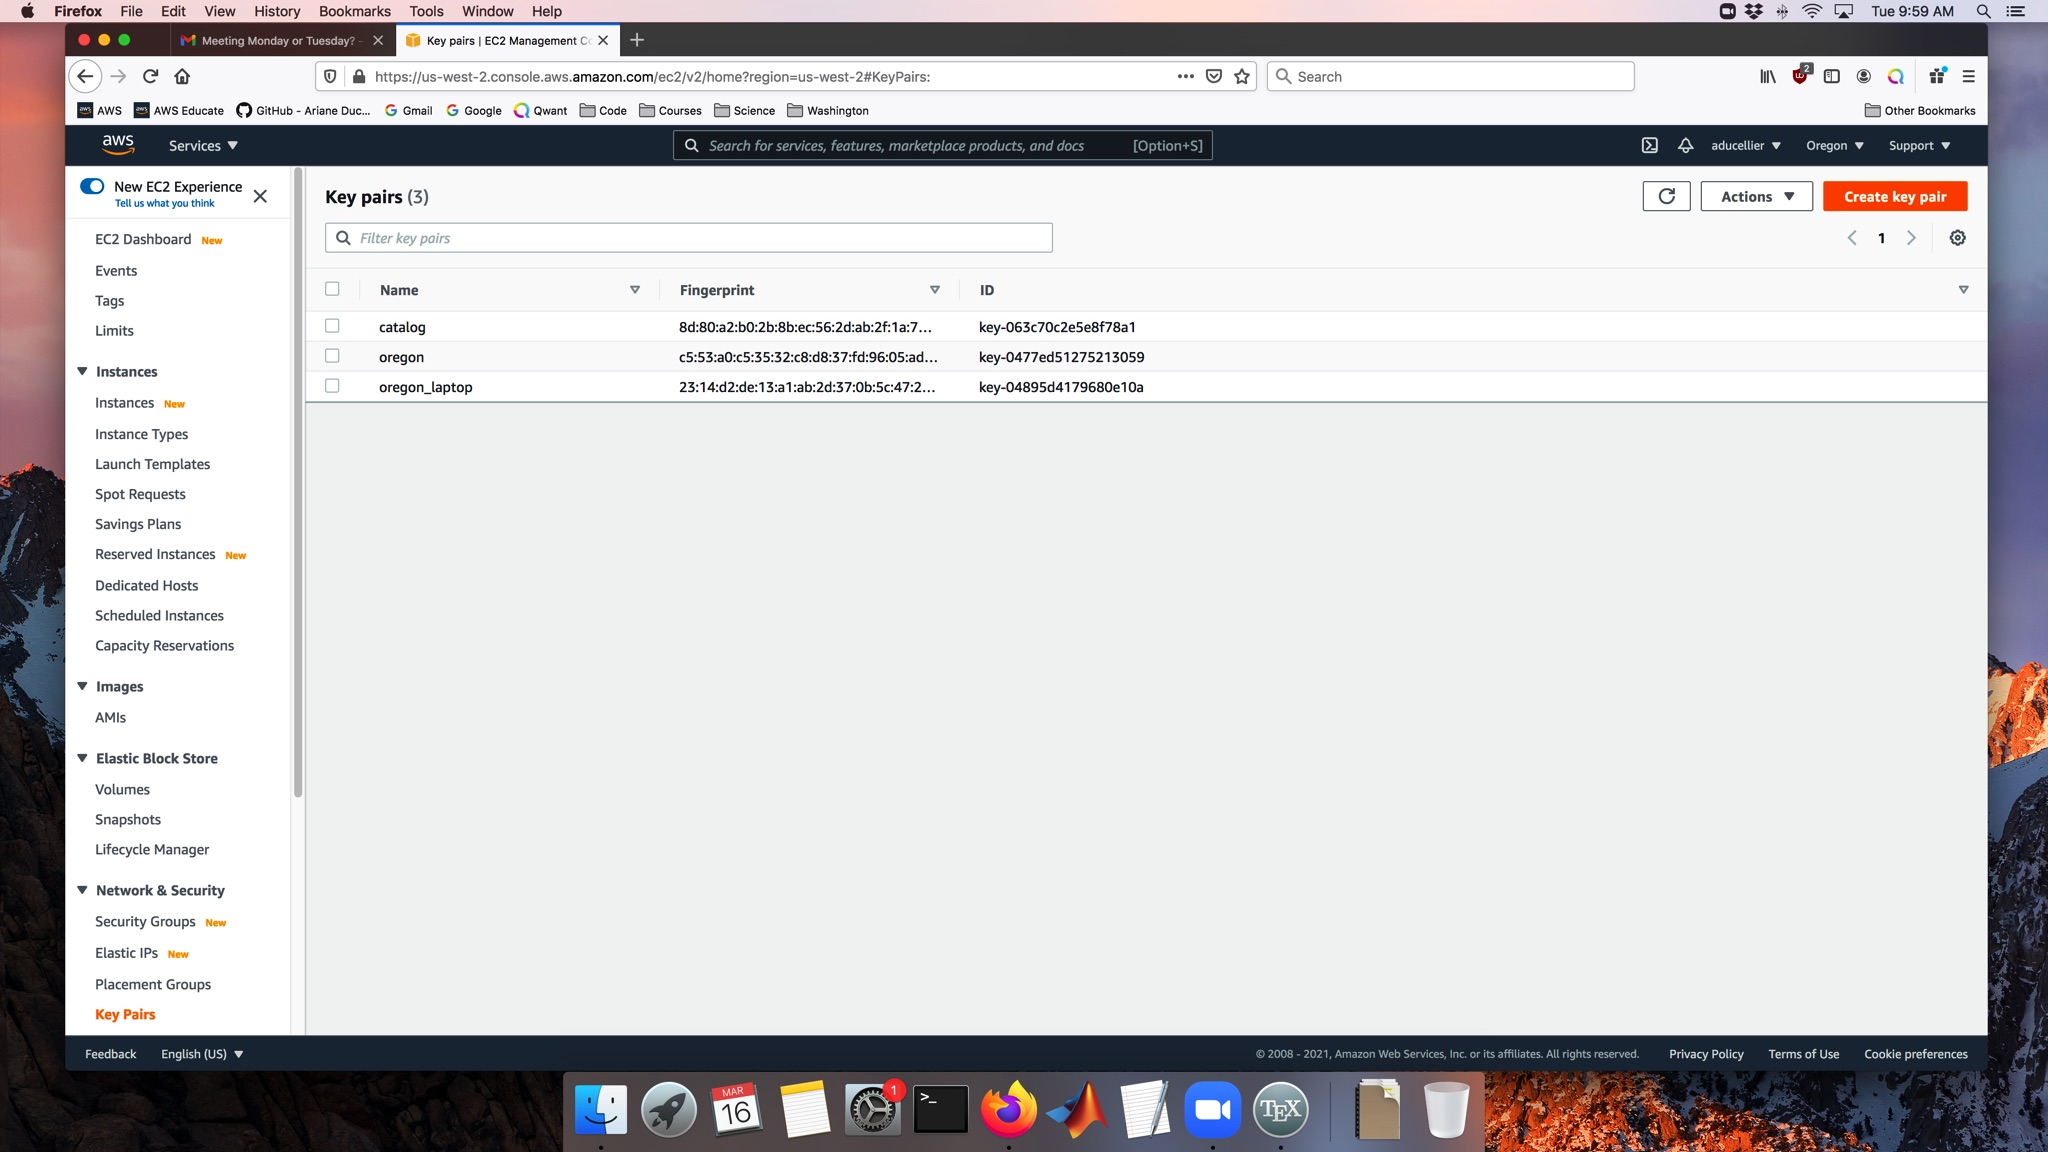
\includegraphics[width=11cm]{figures/list_key_pairs_before.jpg}};
		\draw<1>[red, thick] (9.7,5.0) rectangle ++(0.9,0.3);
	\end{tikzpicture}
	\end{frame}

	\begin{frame}
	\frametitle{Fill in the form and click on \textit{Create key pair}}
	\begin{tikzpicture}
		\node[anchor=south west, inner sep=0] at (0,0) {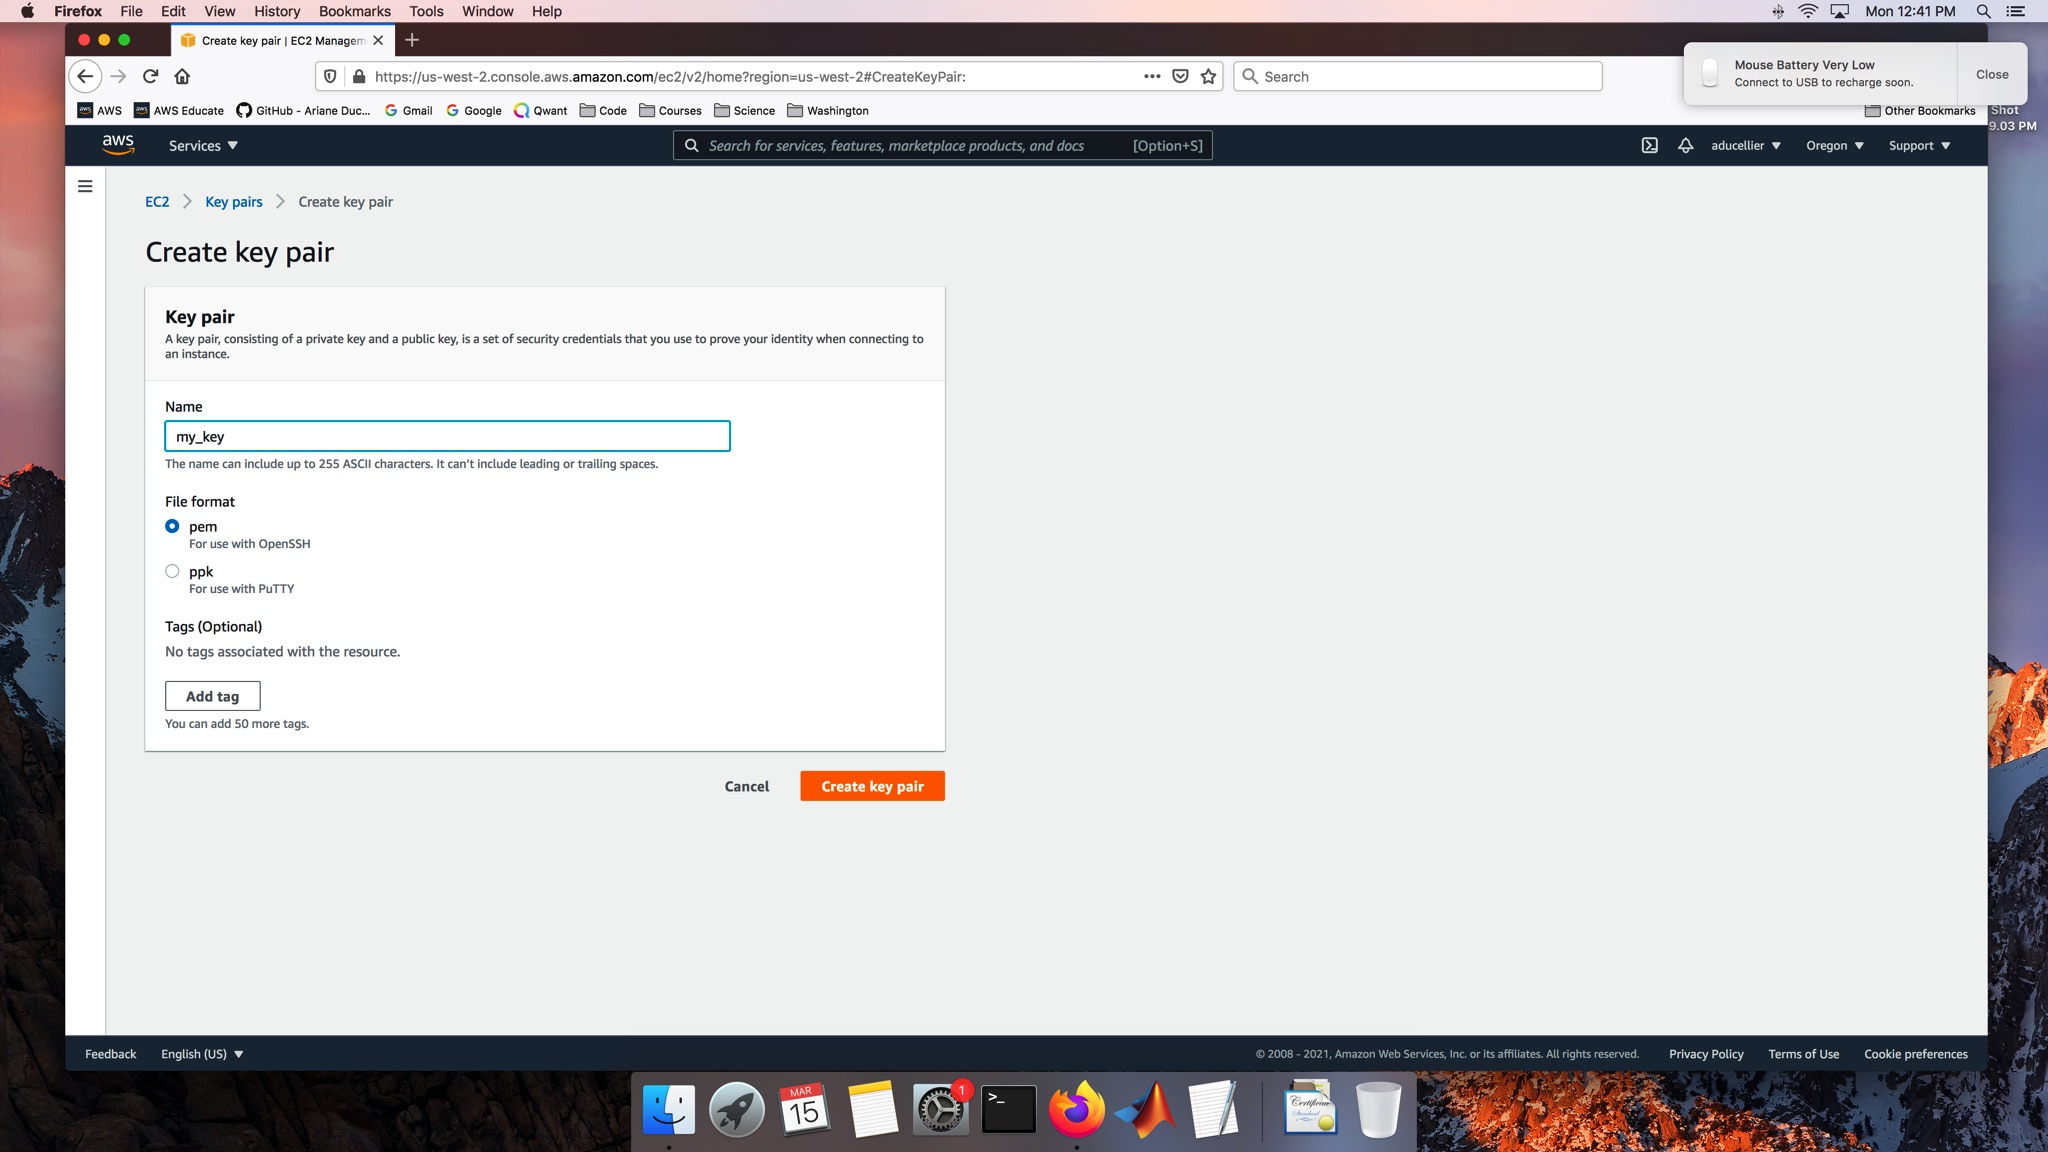
\includegraphics[width=11cm]{figures/create_key_pair.jpg}};
		\draw<1>[red, thick] (4.2,1.8) rectangle ++(1.0,0.3);
	\end{tikzpicture}
	\end{frame}

	\begin{frame}
	\frametitle{Download the file on your machine}
	\begin{tikzpicture}
		\node[anchor=south west, inner sep=0] at (0,0) {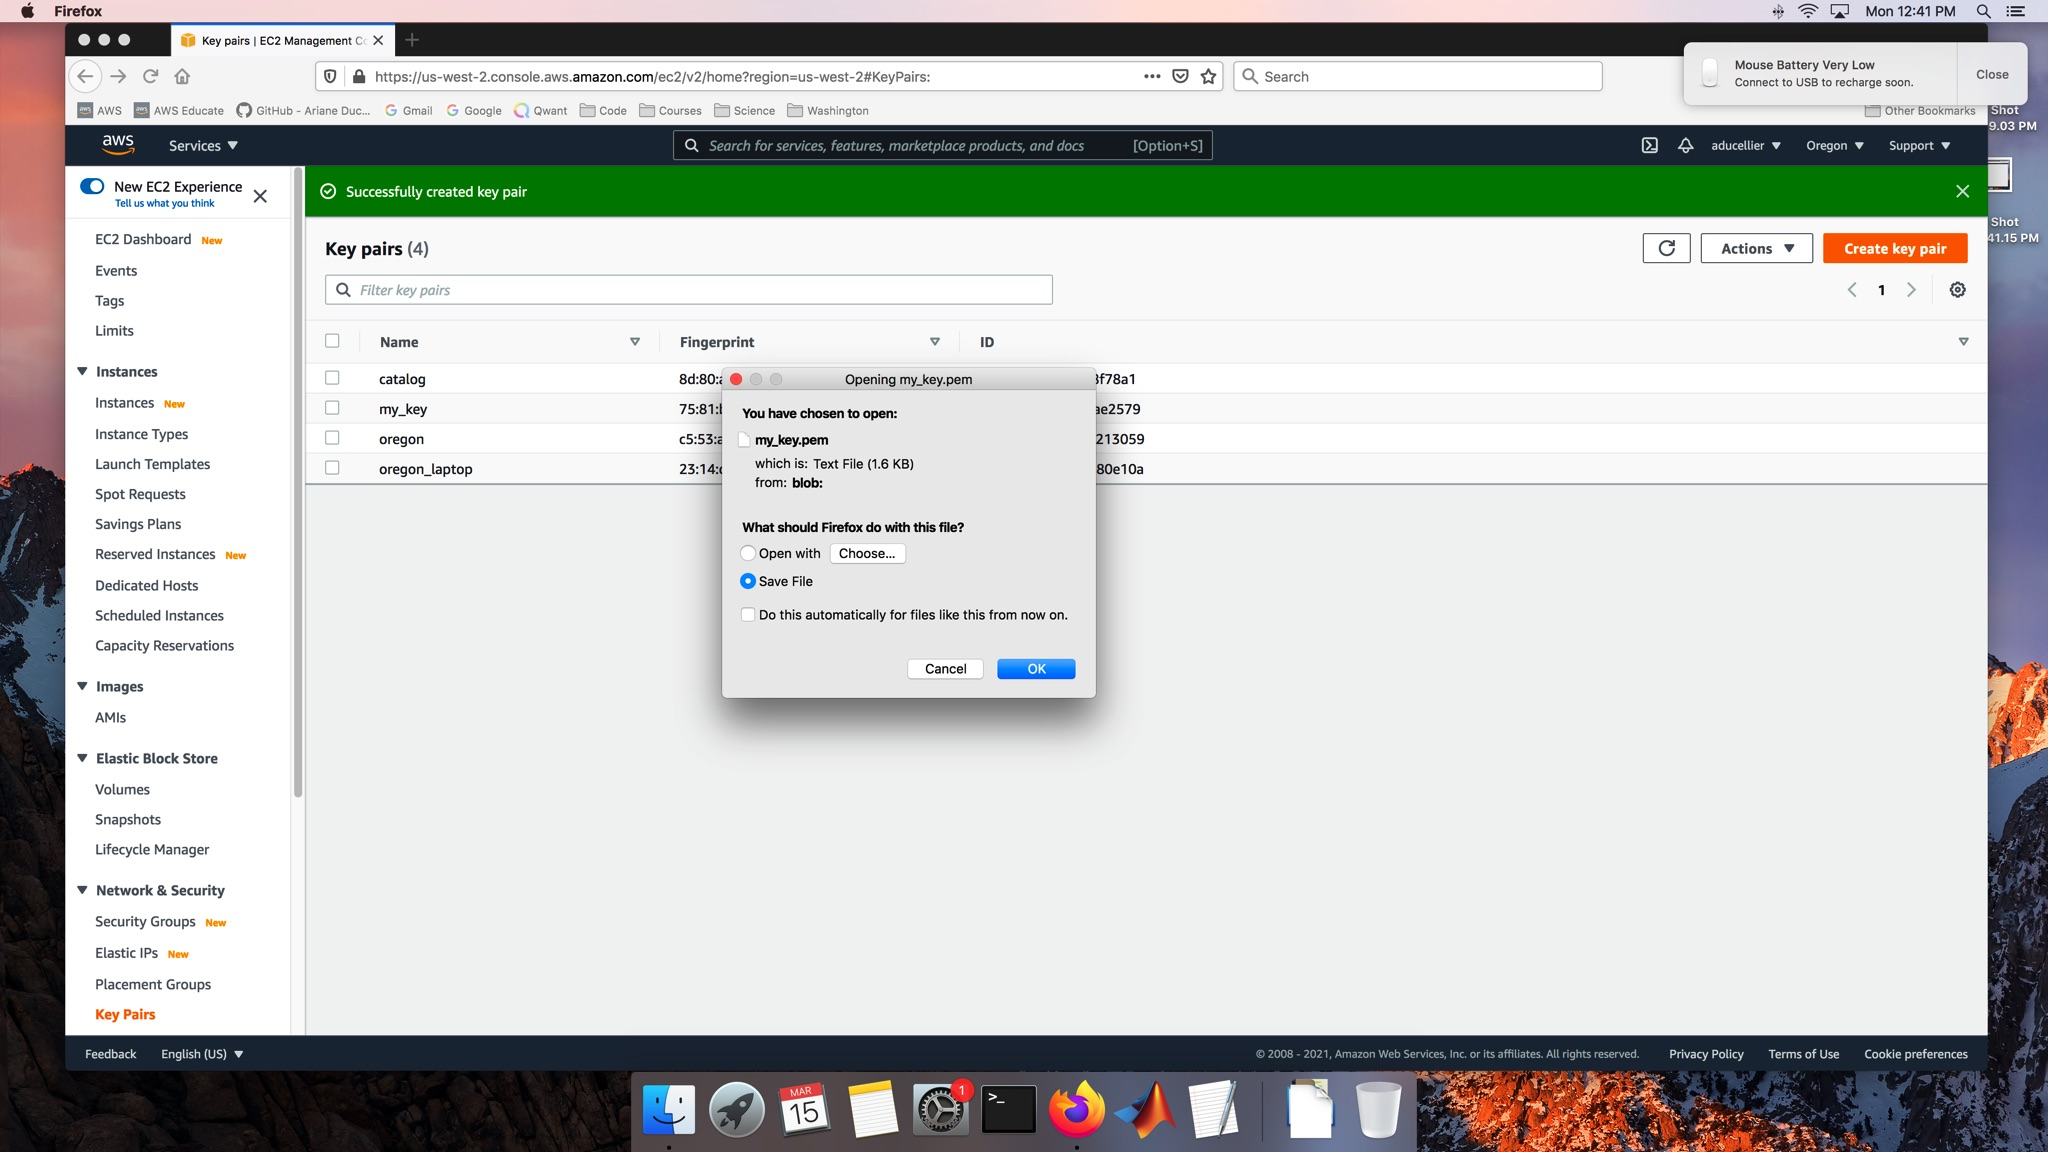
\includegraphics[width=11cm]{figures/download_key_pair.jpg}};
		\draw<1>[red, thick] (5.3,2.4) rectangle ++(0.5,0.3);
	\end{tikzpicture}
	\end{frame}

	\begin{frame}
	\frametitle{Your new key pair appears on the list of available key pairs}
	\begin{tikzpicture}
		\node[anchor=south west, inner sep=0] at (0,0) {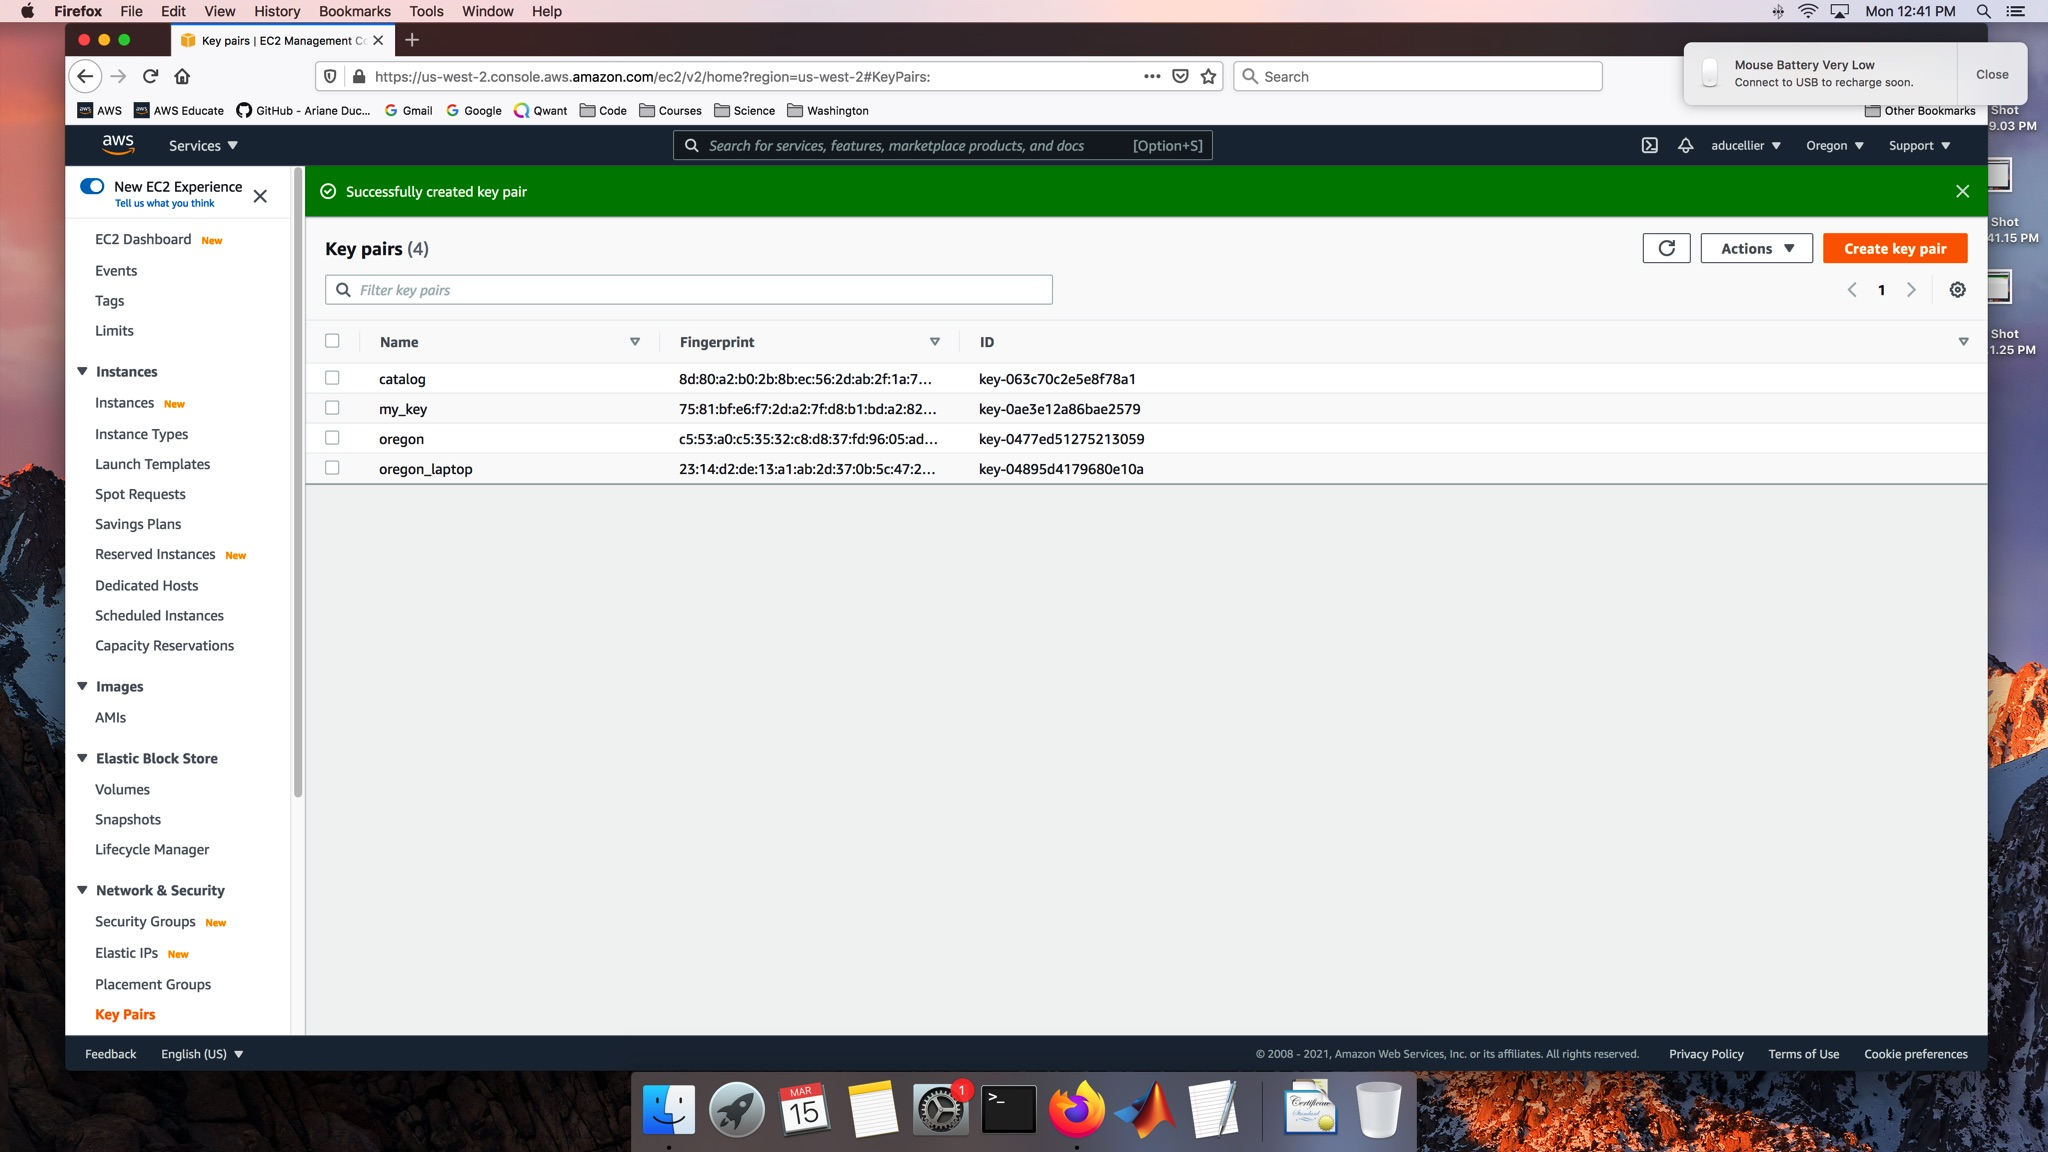
\includegraphics[width=11cm]{figures/list_key_pairs_after.jpg}};
		\draw<1>[red, thick] (1.9,3.9) rectangle ++(0.5,0.2);
	\end{tikzpicture}
	\end{frame}

	\begin{frame}[fragile]
	\frametitle{Move key pair to .ssh for instance}
	\begin{exampleblock}{}
		\begin{verbatim}
		> cd Downloads
		> mv my_key.pem ~/.ssh
		\end{verbatim}
	\end{exampleblock}
	\end{frame}

	\begin{frame}
	\frametitle{Now let us launch a new EC2 instance!}
	\begin{tikzpicture}
		\node[anchor=south west, inner sep=0] at (0,0) {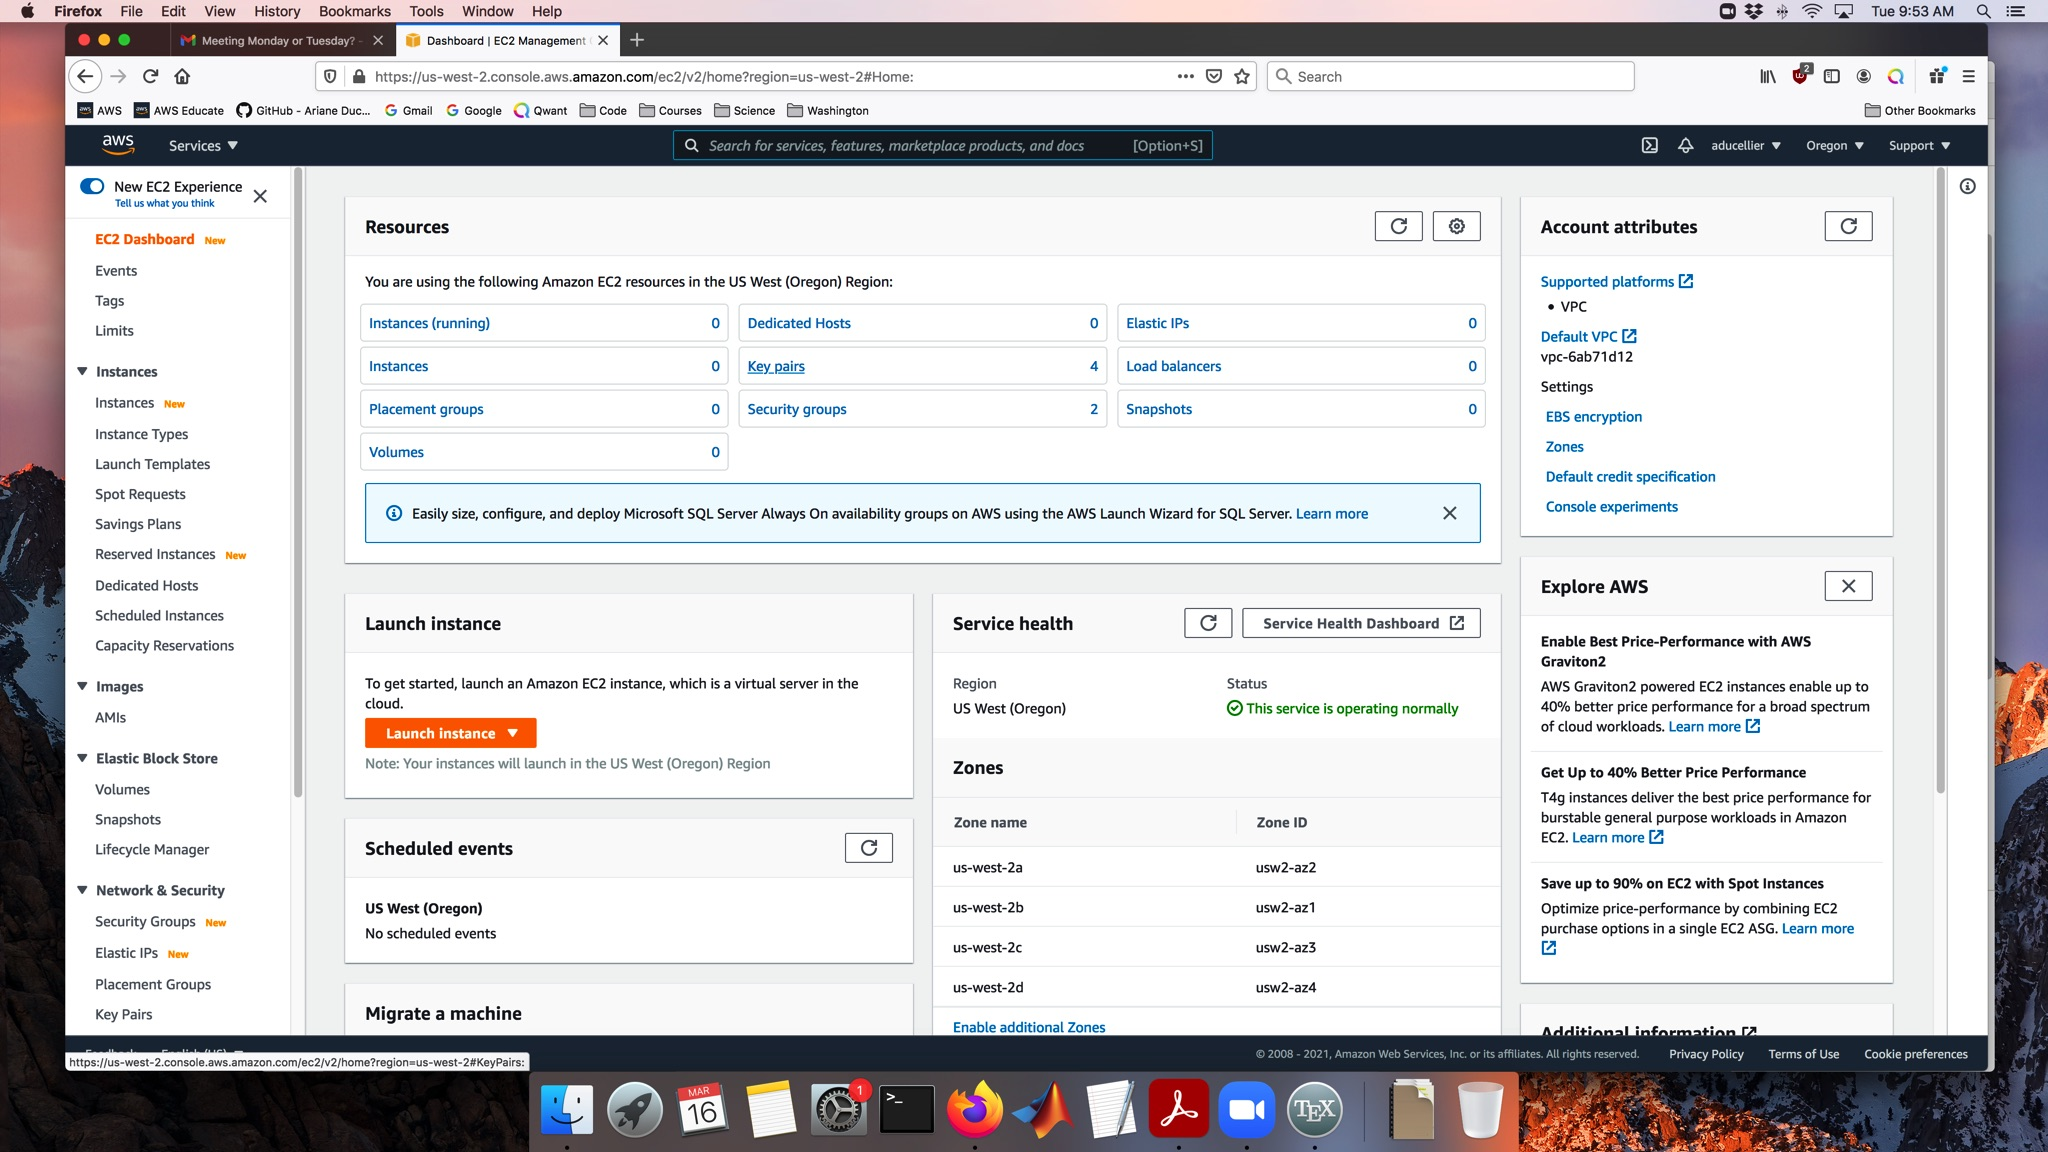
\includegraphics[width=11cm]{figures/EC2_home.jpg}};
		\draw<1>[red, thick] (1.9,2.1) rectangle ++(1.1,0.3);
	\end{tikzpicture}
	\end{frame}

	\begin{frame}
	\frametitle{You first need to choose an Amazon Machine Image (AMI)}
	\begin{tikzpicture}
		\node[anchor=south west, inner sep=0] at (0,0) {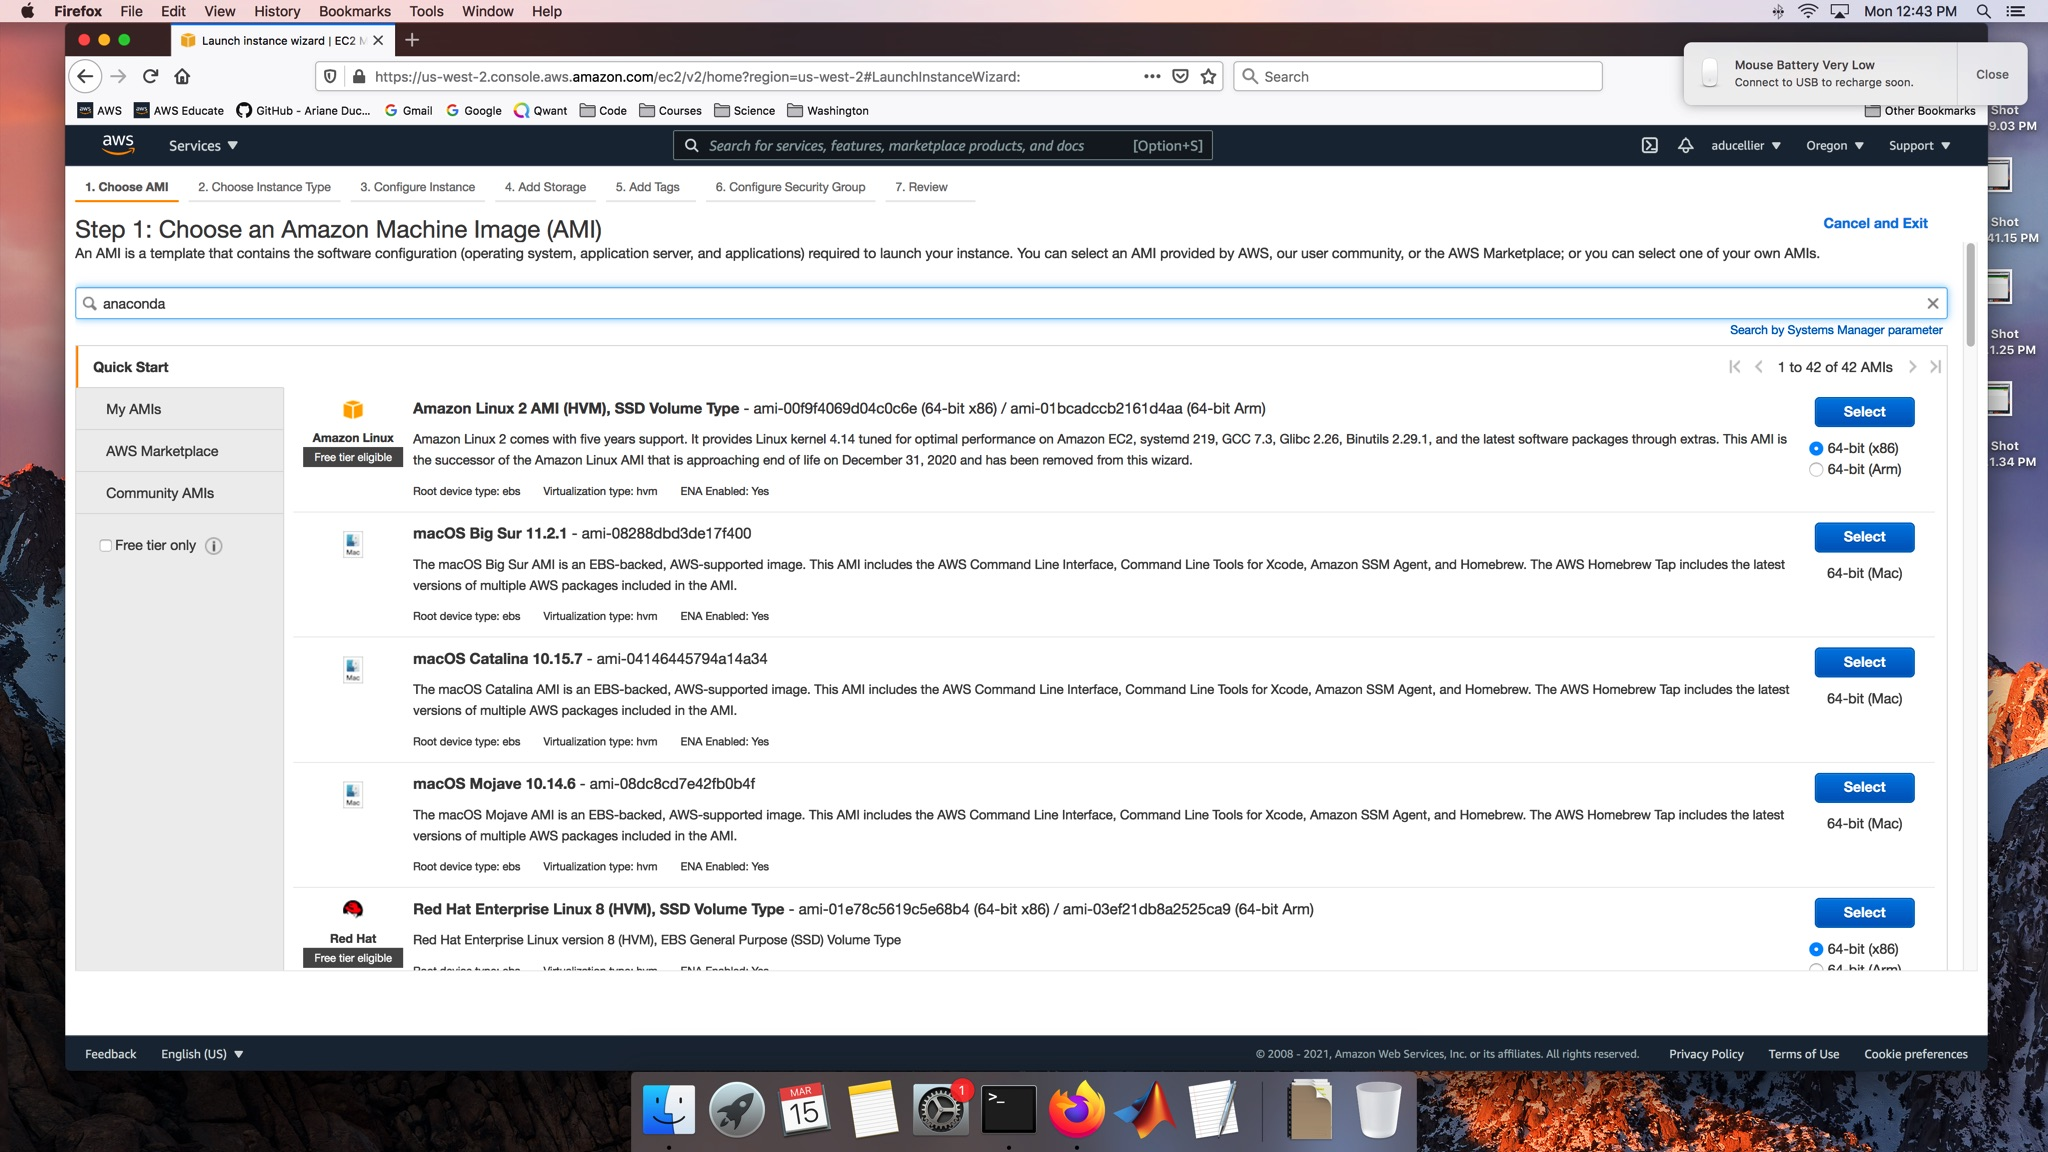
\includegraphics[width=11cm]{figures/choose_AMI.jpg}};
		\draw<1>[red, thick] (0.5,4.4) rectangle ++(0.5,0.3);
	\end{tikzpicture}
	\end{frame}

	\begin{frame}
	\frametitle{We want one with Anaconda installed}
	\begin{tikzpicture}
		\node[anchor=south west, inner sep=0] at (0,0) {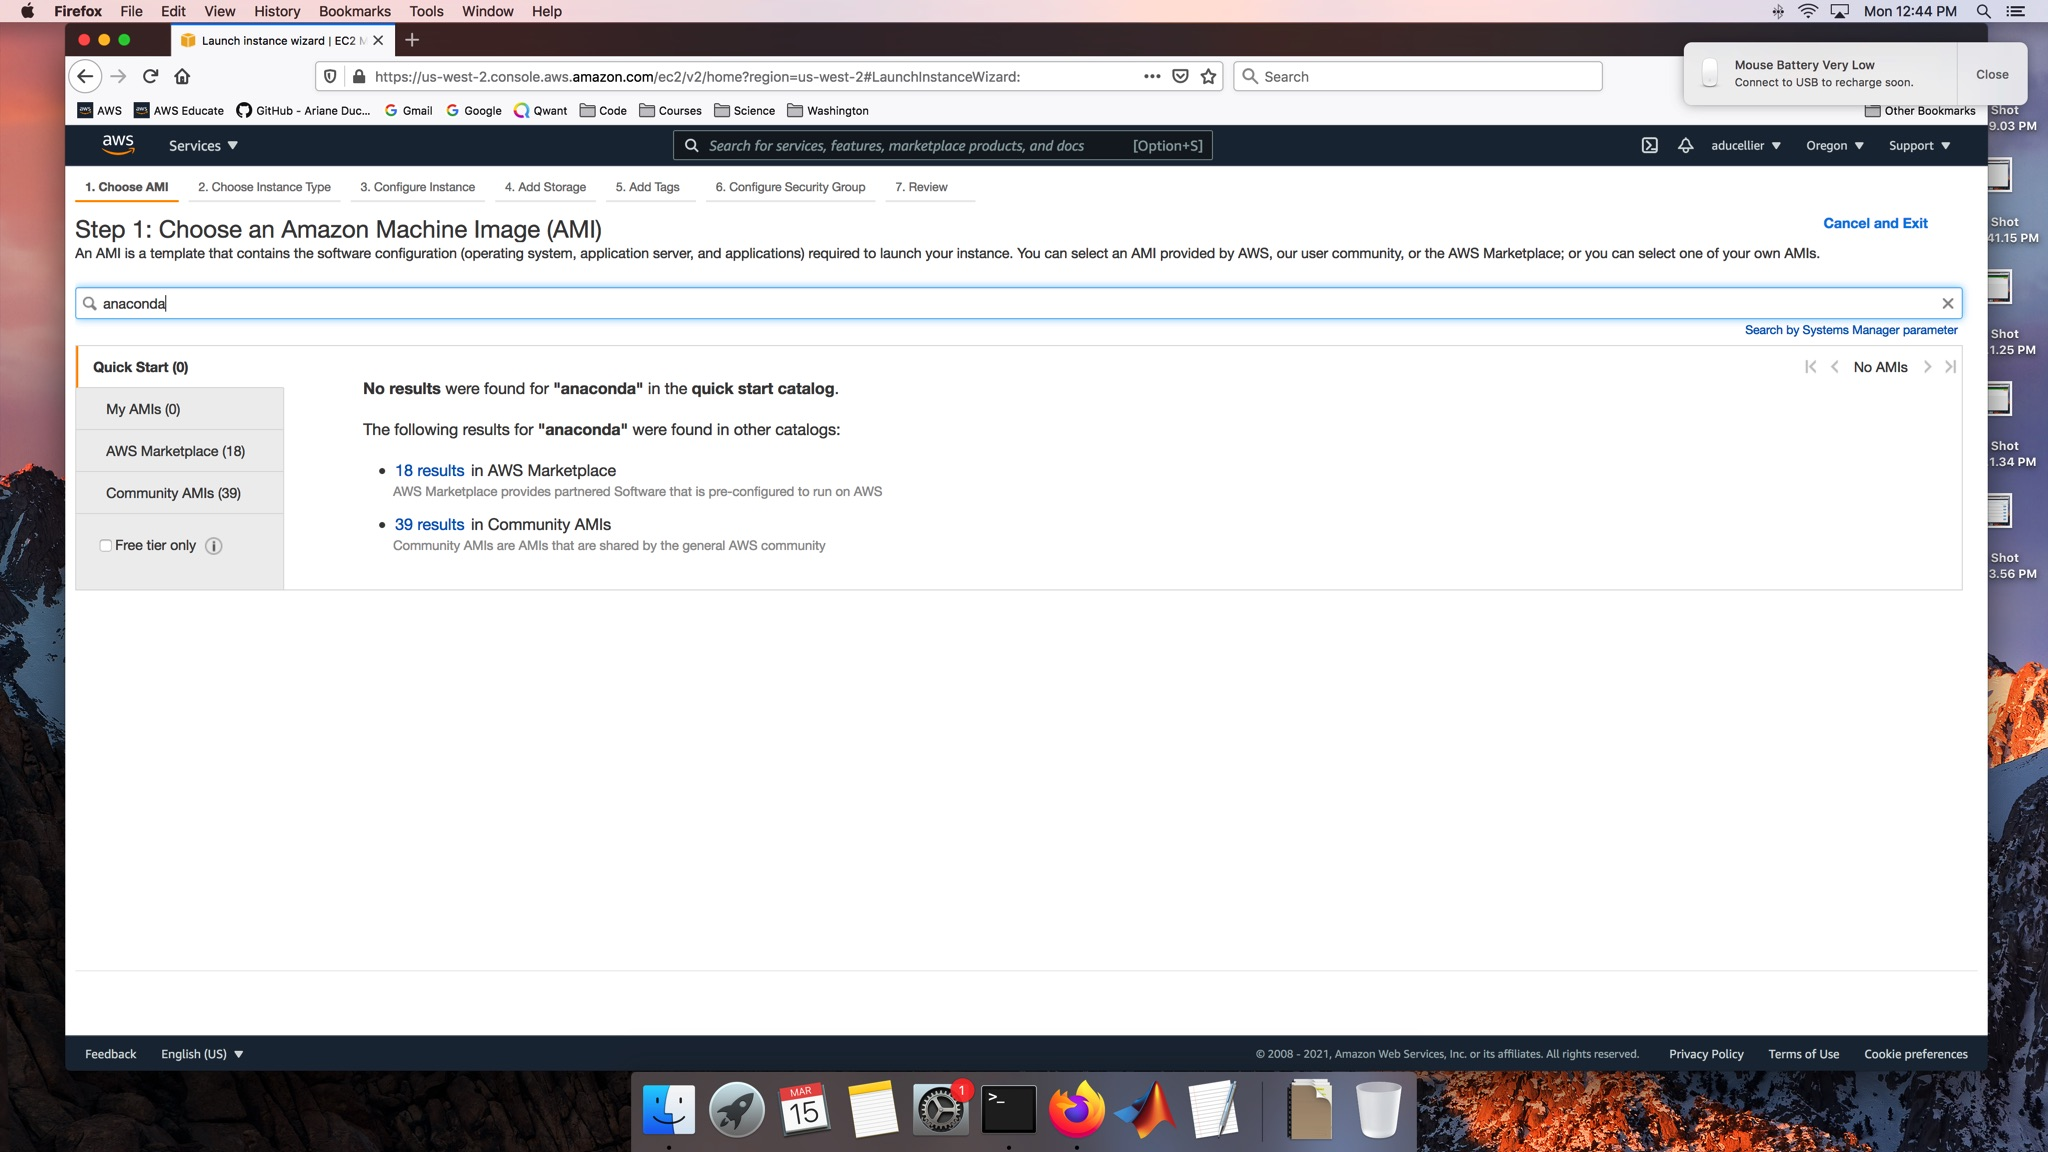
\includegraphics[width=11cm]{figures/choose_anaconda_AMIs.jpg}};
		\draw<1>[red, thick] (2.1,3.5) rectangle ++(0.5,0.3);
	\end{tikzpicture}
	\end{frame}

	\begin{frame}
	\frametitle{We choose the one with Anaconda and Python 3}
	\begin{tikzpicture}
		\node[anchor=south west, inner sep=0] at (0,0) {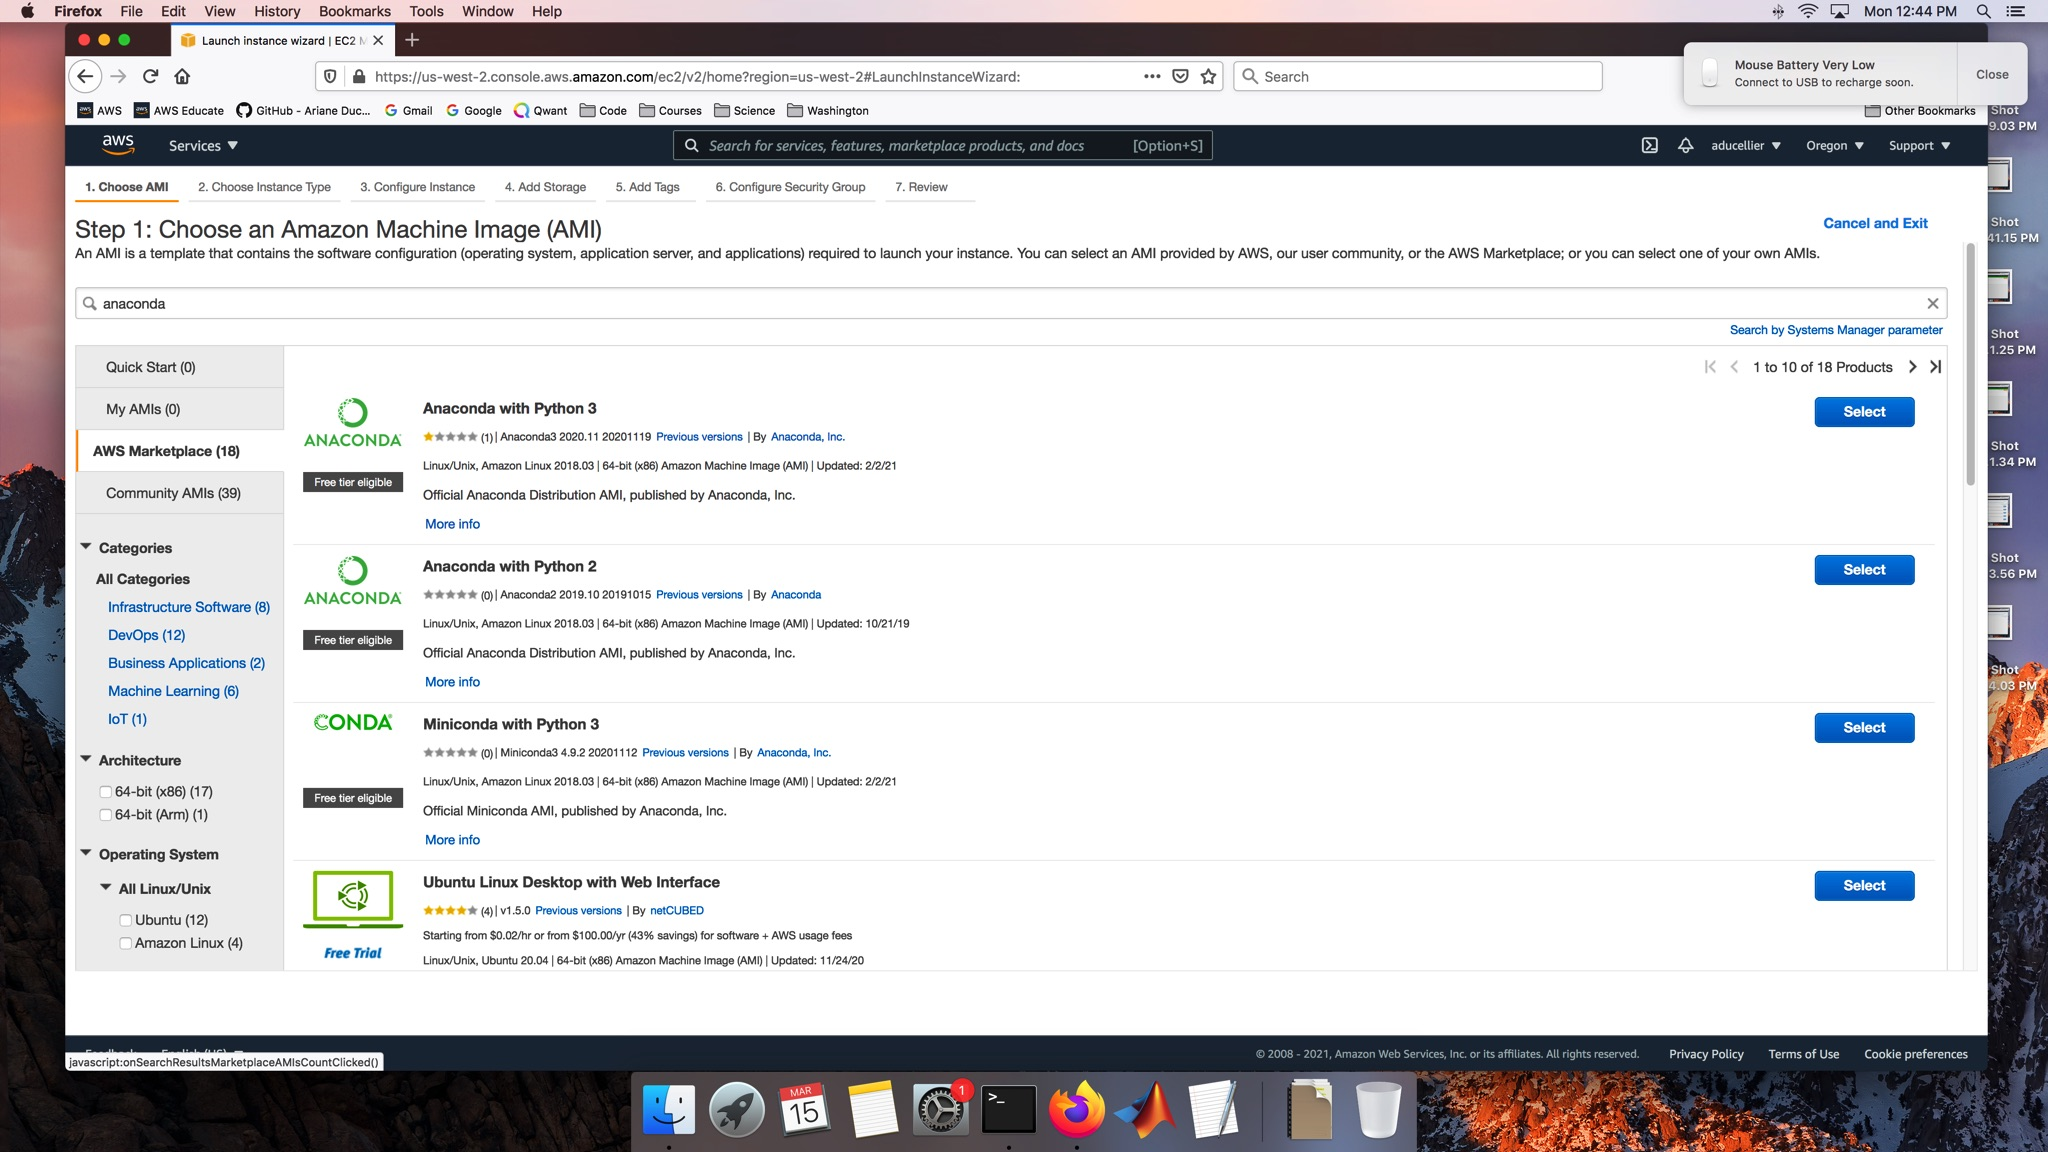
\includegraphics[width=11cm]{figures/select_anaconda_python3.jpg}};
		\draw<1>[red, thick] (2.2,3.9) rectangle ++(1.1,0.3);
		\draw<1>[red, thick] (9.7,3.8) rectangle ++(0.7,0.3);
	\end{tikzpicture}
	\end{frame}

	\begin{frame}
	\frametitle{Check the cost of each type of instance before choosing one}
	\begin{tikzpicture}
		\node[anchor=south west, inner sep=0] at (0,0) {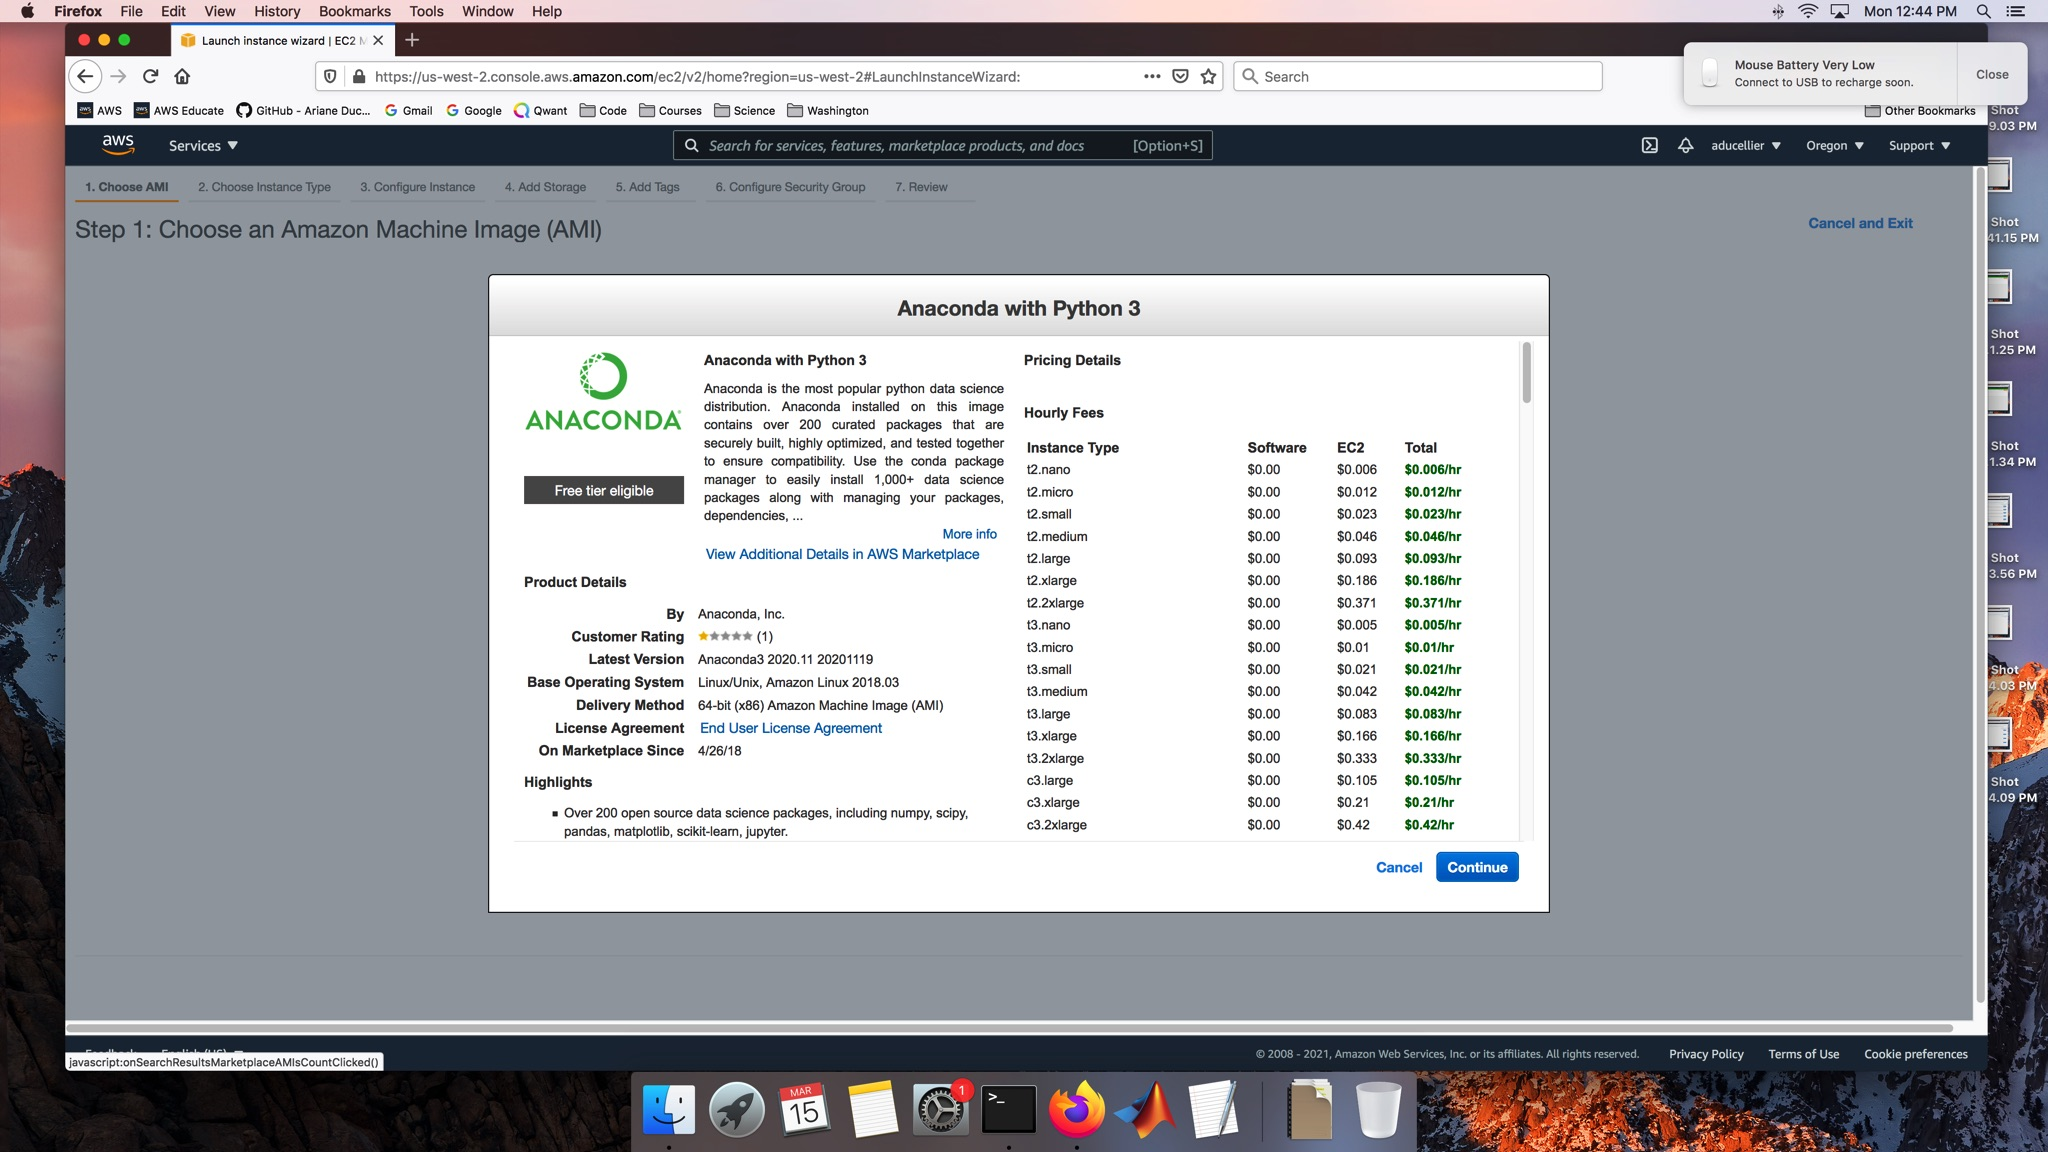
\includegraphics[width=11cm]{figures/list_of_prices.jpg}};
		\draw<1>[red, thick] (7.6,1.4) rectangle ++(0.7,0.3);
	\end{tikzpicture}
	\end{frame}

	\begin{frame}
	\frametitle{Select the type of instance you want: We choose t3.small}
	\begin{tikzpicture}
		\node[anchor=south west, inner sep=0] at (0,0) {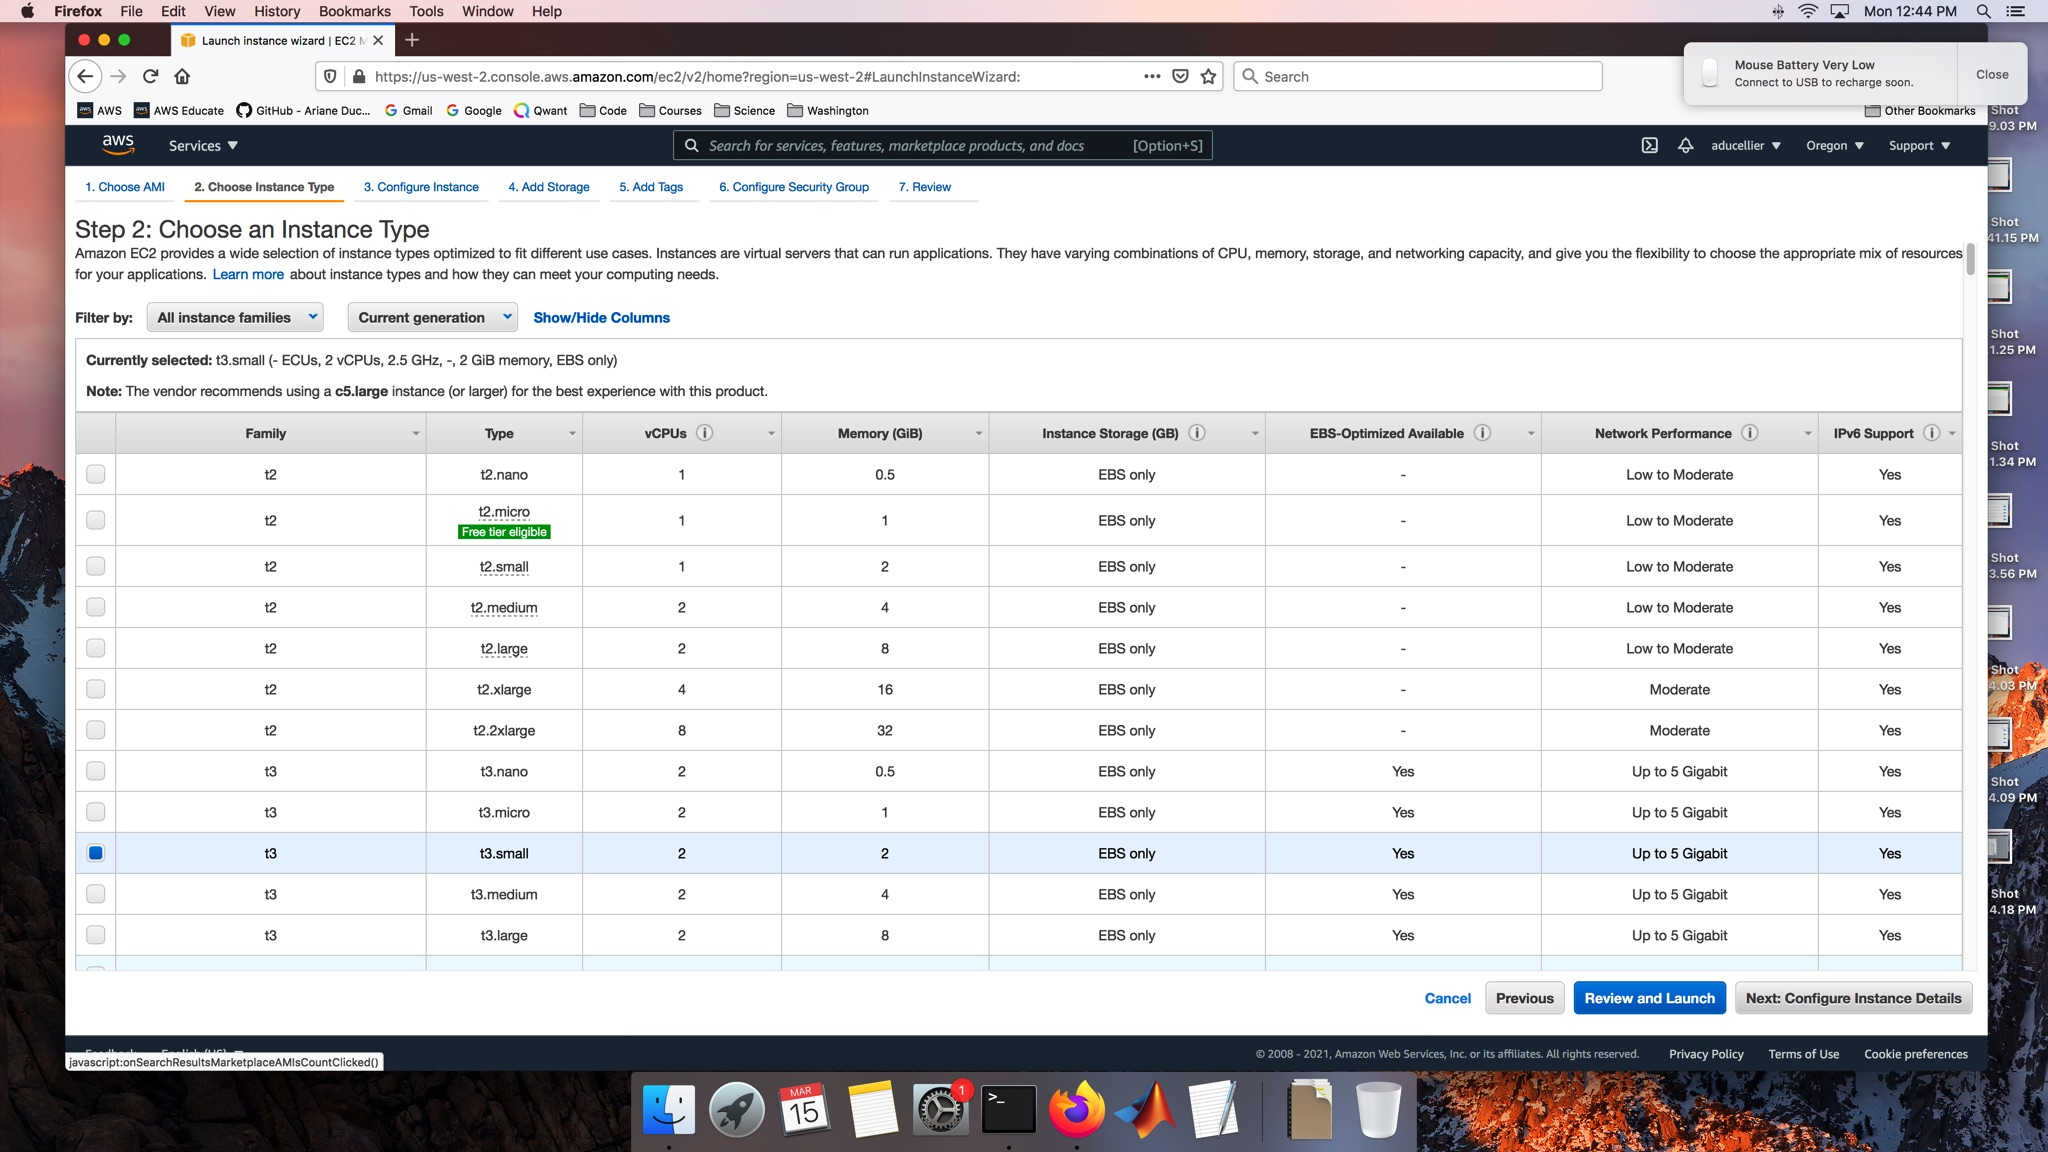
\includegraphics[width=11cm]{figures/choose_instance_type.jpg}};
		\draw<1>[red, thick] (0.4,1.5) rectangle ++(0.2,0.2);
	\end{tikzpicture}
	\end{frame}

	\begin{frame}
	\frametitle{Configure the instance (you can leave it as it is)}
	\begin{tikzpicture}
		\node[anchor=south west, inner sep=0] at (0,0) {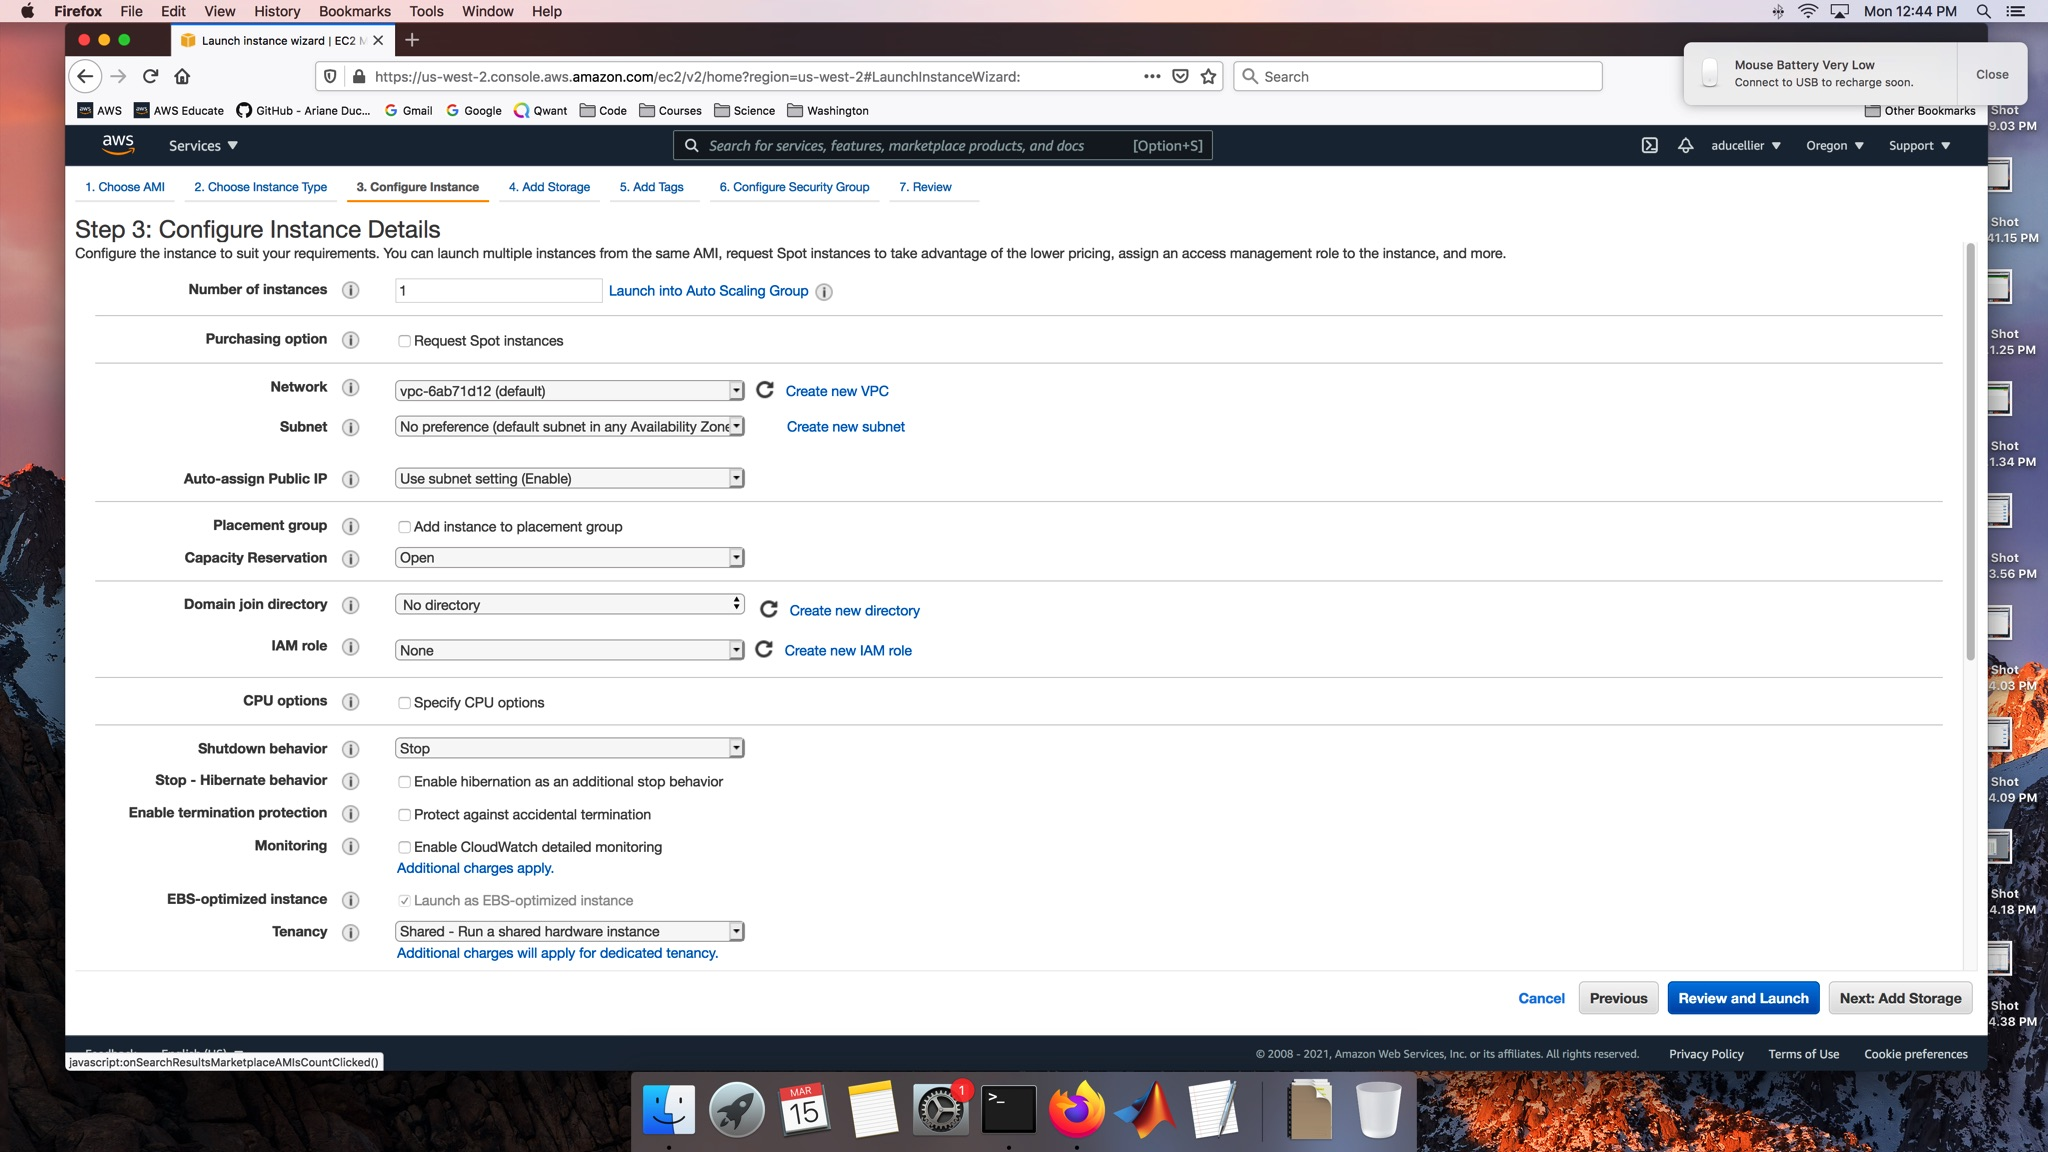
\includegraphics[width=11cm]{figures/configure_instance.jpg}};
		\draw<1>[red, thick] (9.8,0.7) rectangle ++(0.8,0.3);
	\end{tikzpicture}
	\end{frame}

	\begin{frame}
	\frametitle{Choose the storage (you can leave it as it is)}
	\begin{tikzpicture}
		\node[anchor=south west, inner sep=0] at (0,0) {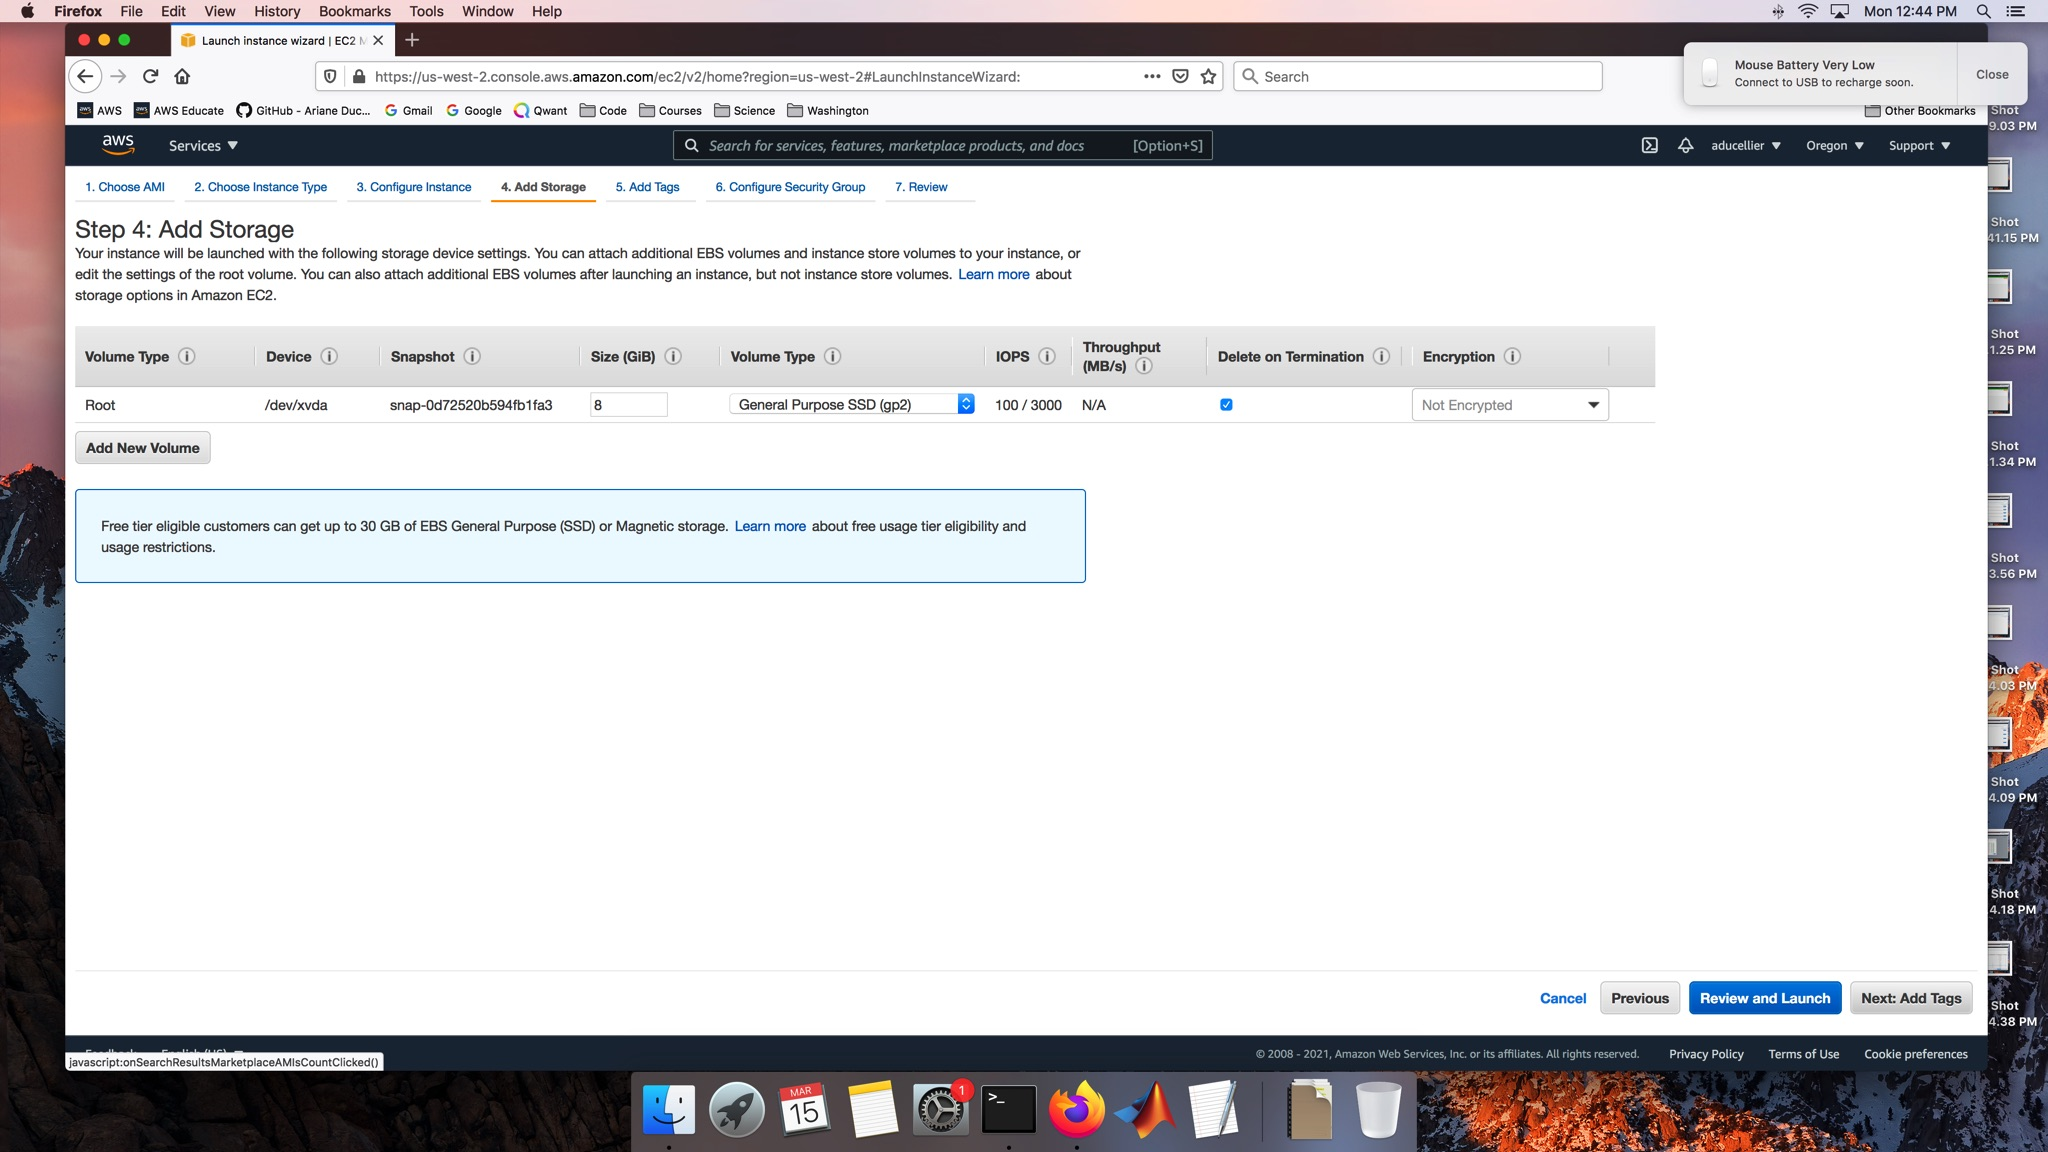
\includegraphics[width=11cm]{figures/add_storage.jpg}};
		\draw<1>[red, thick] (9.9,0.7) rectangle ++(0.8,0.3);
	\end{tikzpicture}
	\end{frame}

	\begin{frame}
	\frametitle{Add tags to remember what jobs you will be running on your EC2 instance}
	\begin{tikzpicture}
		\node[anchor=south west, inner sep=0] at (0,0) {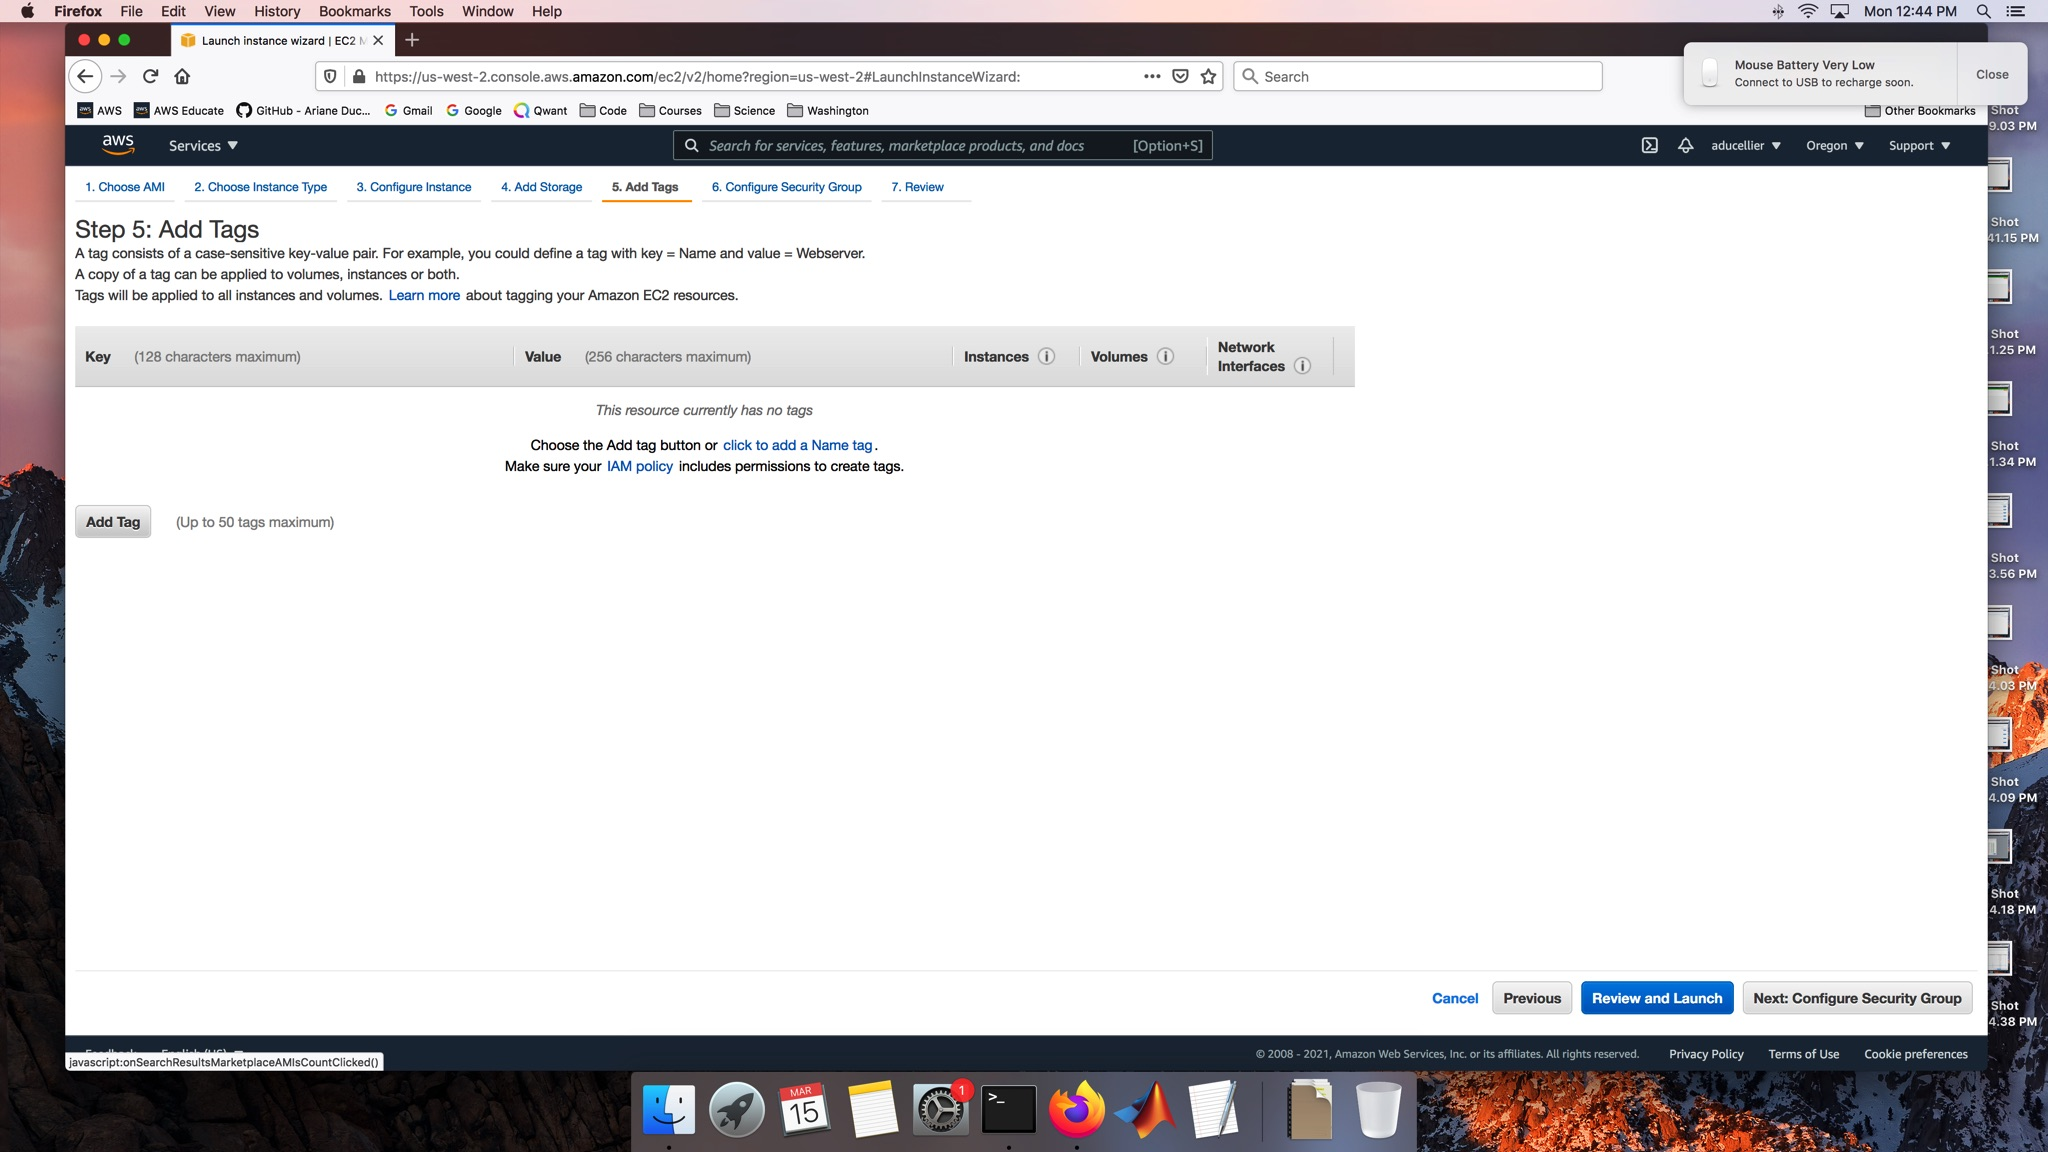
\includegraphics[width=11cm]{figures/add_tags.jpg}};
		\draw<1>[red, thick] (0.3,3.3) rectangle ++(0.6,0.3);
	\end{tikzpicture}
	\end{frame}

	\begin{frame}
	\frametitle{I want to run the Python script \textit{find\_all\_LFEs\_parallel.py}}
	\begin{tikzpicture}
		\node[anchor=south west, inner sep=0] at (0,0) {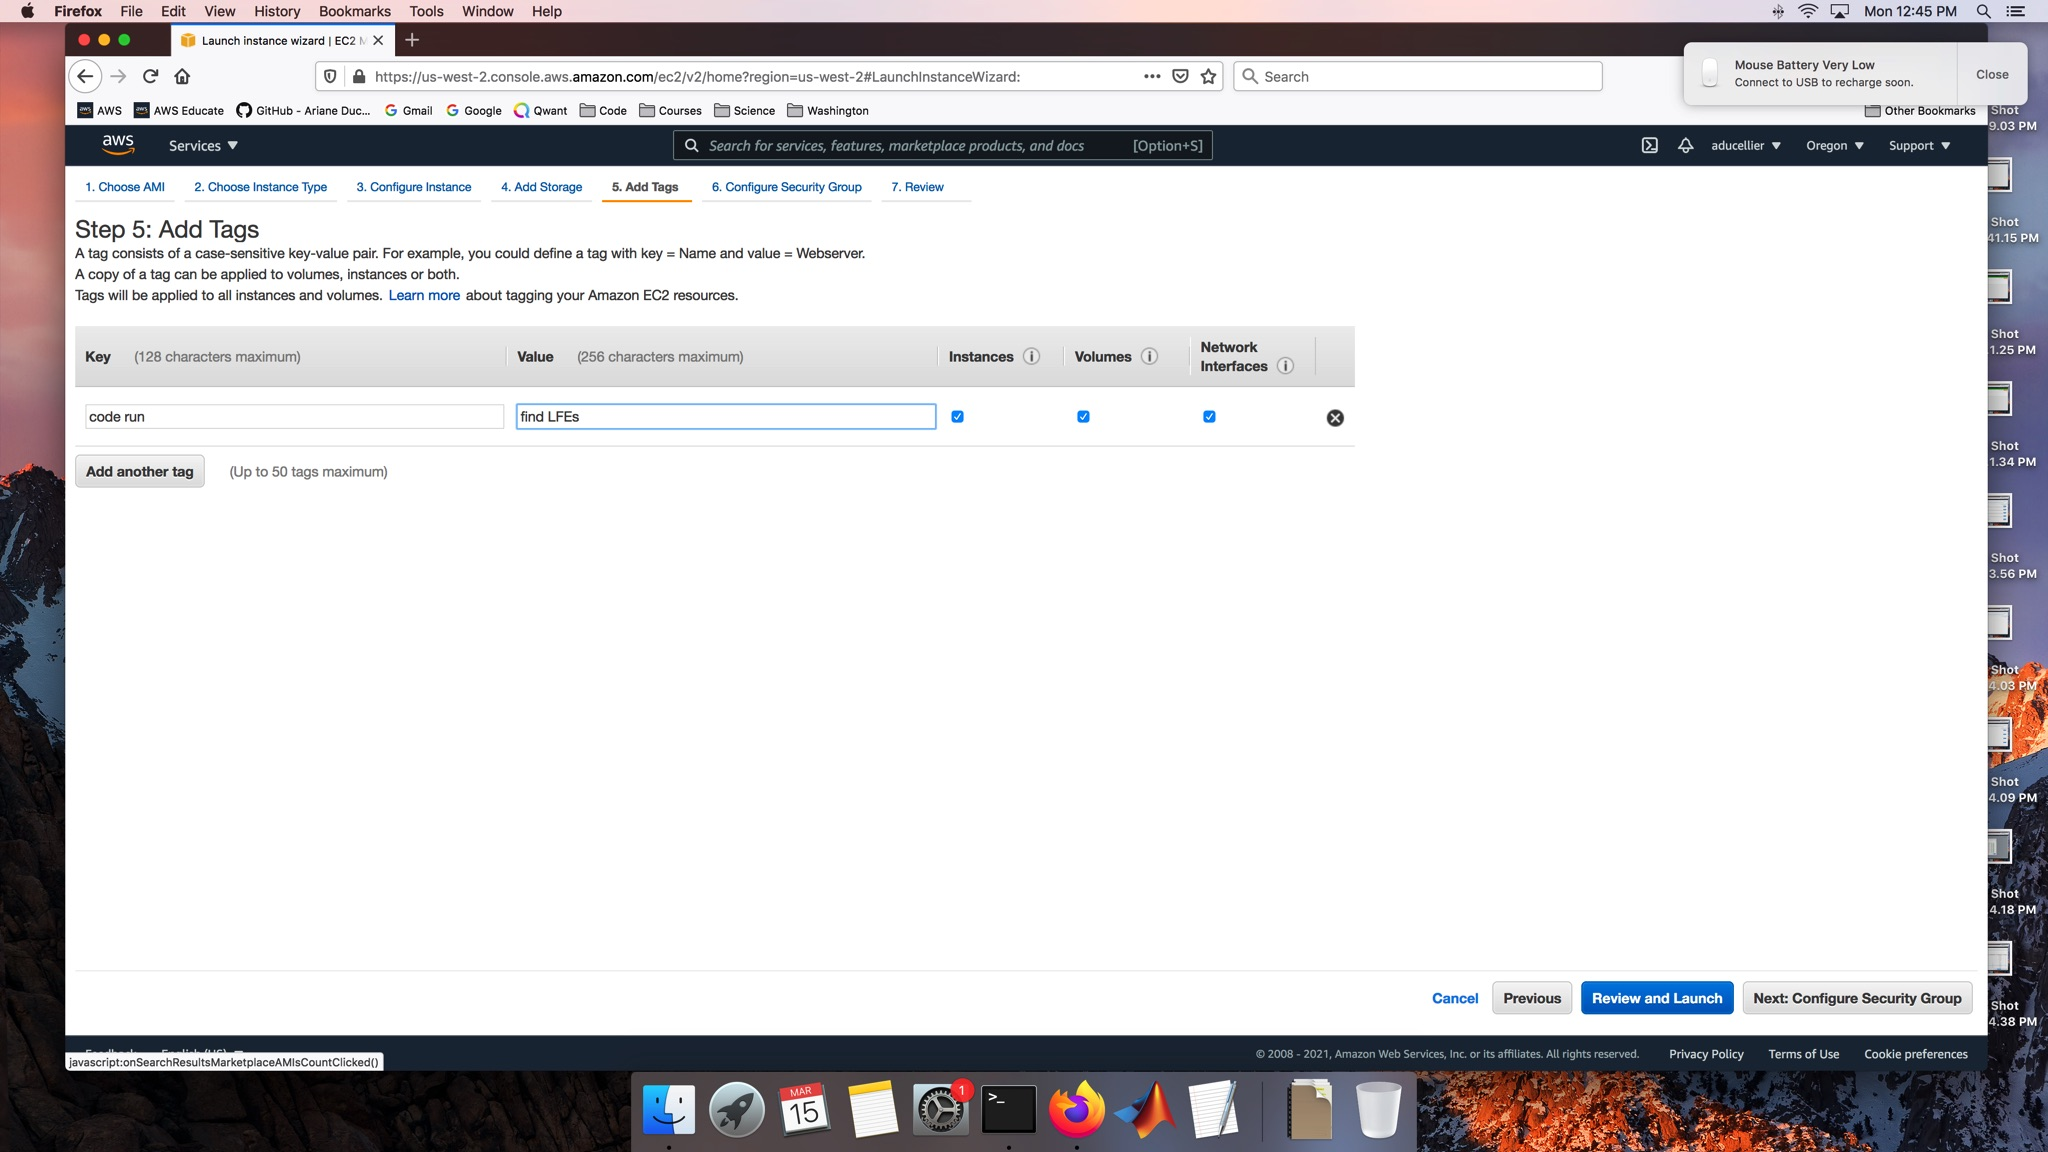
\includegraphics[width=11cm]{figures/enter_tag.jpg}};
		\draw<1>[red, thick] (9.3,0.7) rectangle ++(1.4,0.3);
	\end{tikzpicture}
	\end{frame}

	\begin{frame}
	\frametitle{Choose a security group (you can use the same for several instances)}
	\begin{tikzpicture}
		\node[anchor=south west, inner sep=0] at (0,0) {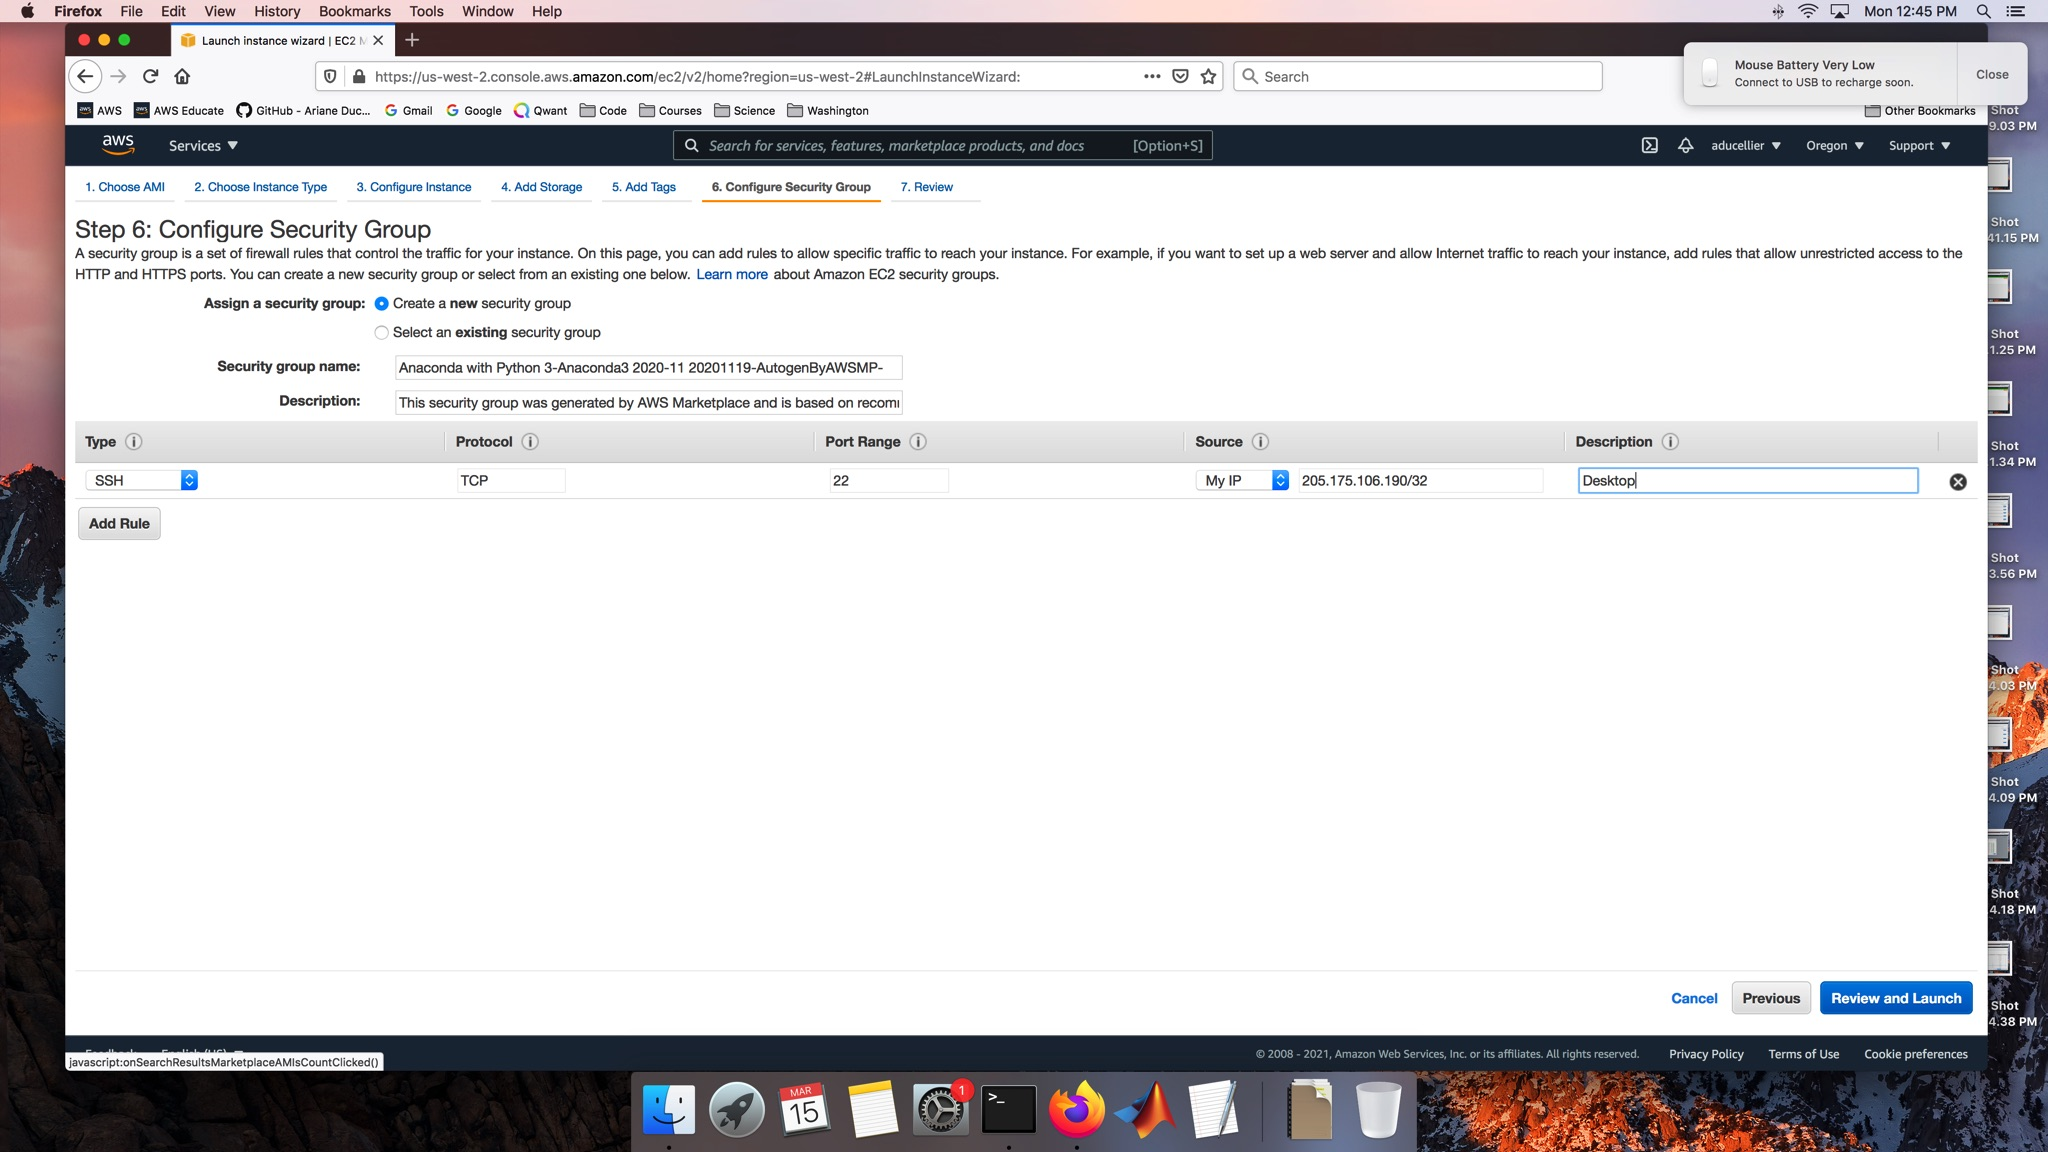
\includegraphics[width=11cm]{figures/choose_security_group.jpg}};
		\draw<1>[red, thick] (6.3,3.5) rectangle ++(0.7,0.3);
		\draw<1>[red, thick] (9.7,0.7) rectangle ++(1.0,0.3);
	\end{tikzpicture}
	\end{frame}

	\begin{frame}
	\frametitle{Review your options before launching}
	\begin{tikzpicture}
		\node[anchor=south west, inner sep=0] at (0,0) {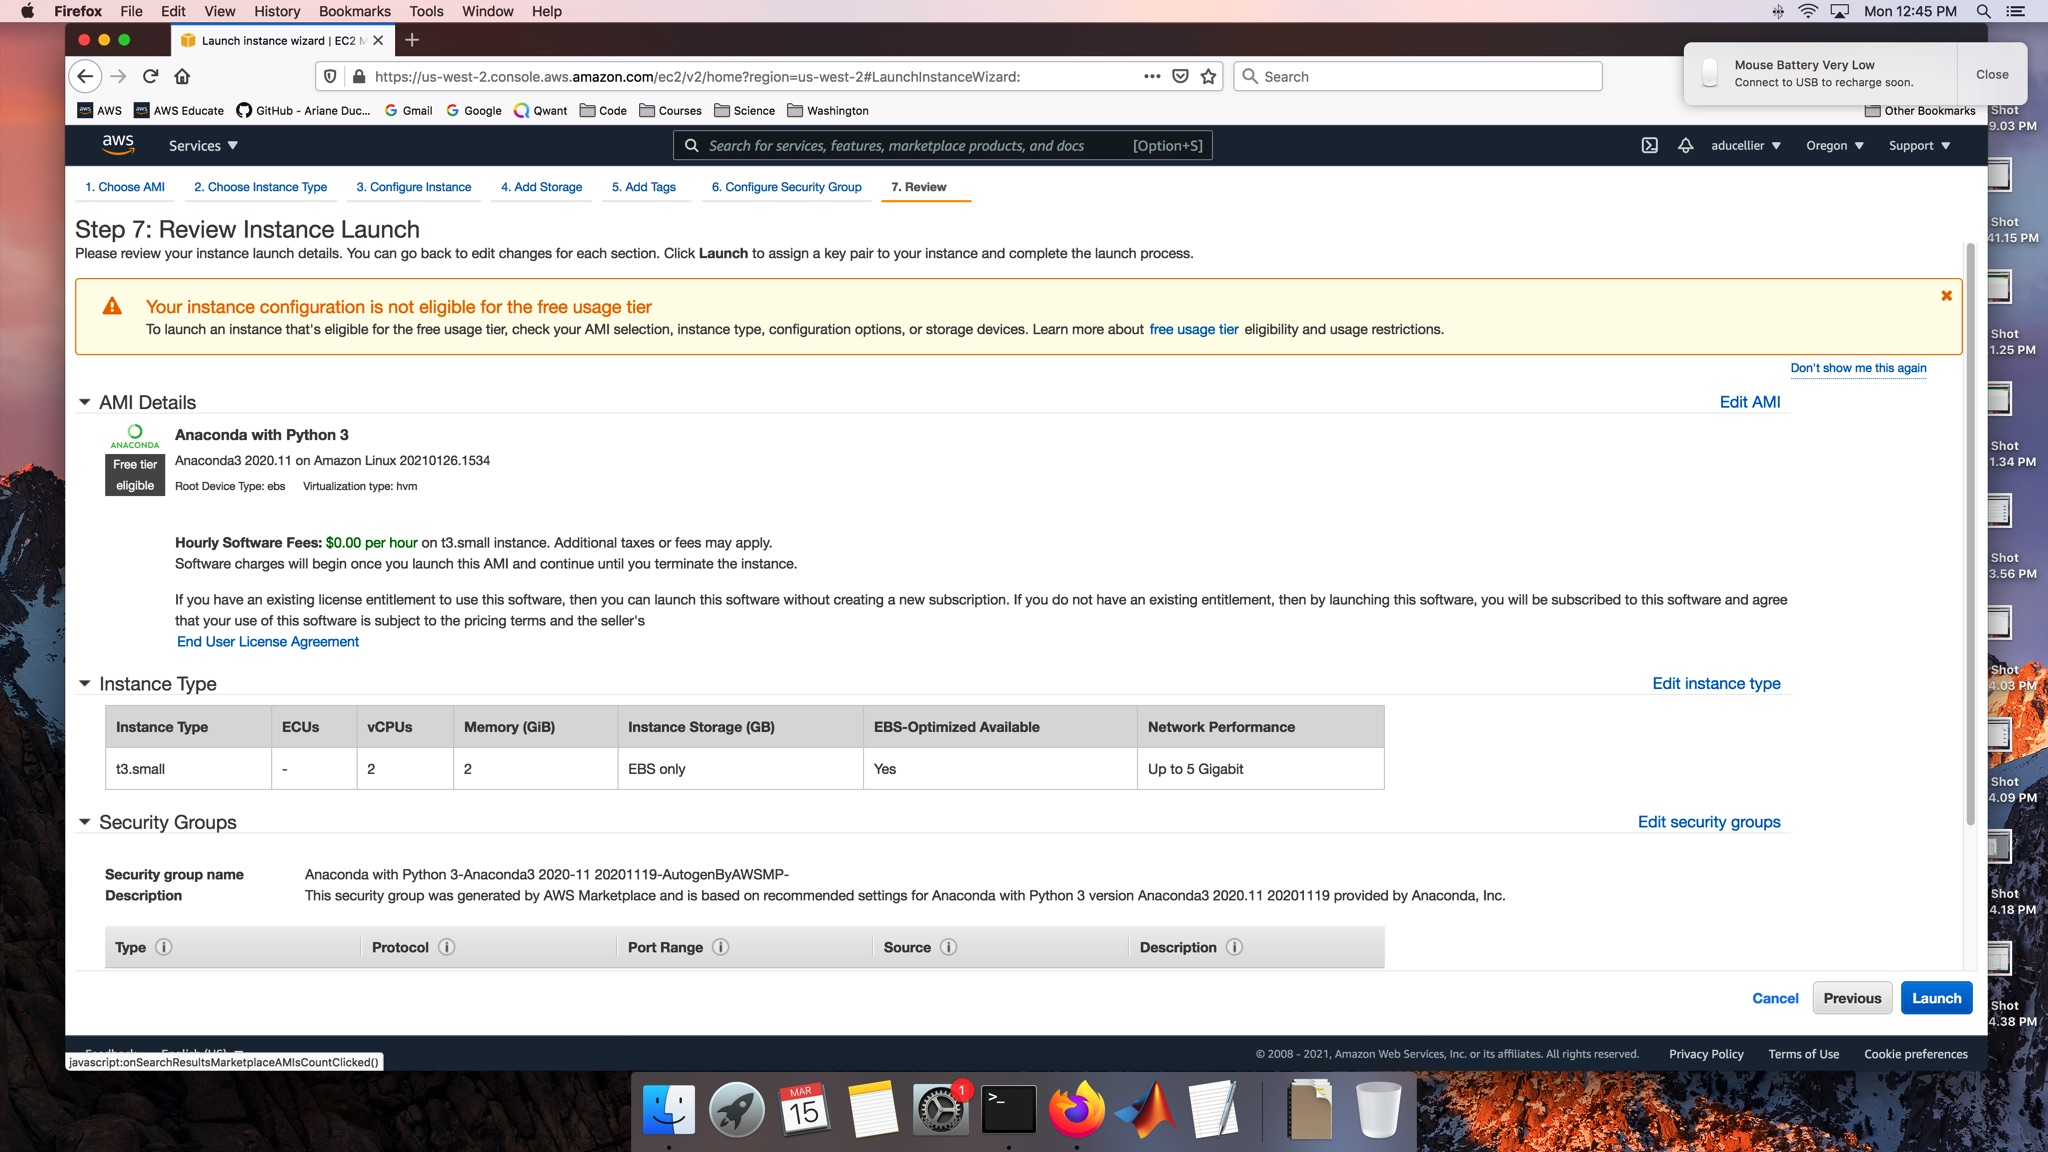
\includegraphics[width=11cm]{figures/review_launch.jpg}};
		\draw<1>[red, thick] (10.1,0.7) rectangle ++(0.6,0.3);
	\end{tikzpicture}
	\end{frame}

	\begin{frame}
	\frametitle{Choose a key pair: the one you have downloaded earlier}
	\begin{tikzpicture}
		\node[anchor=south west, inner sep=0] at (0,0) {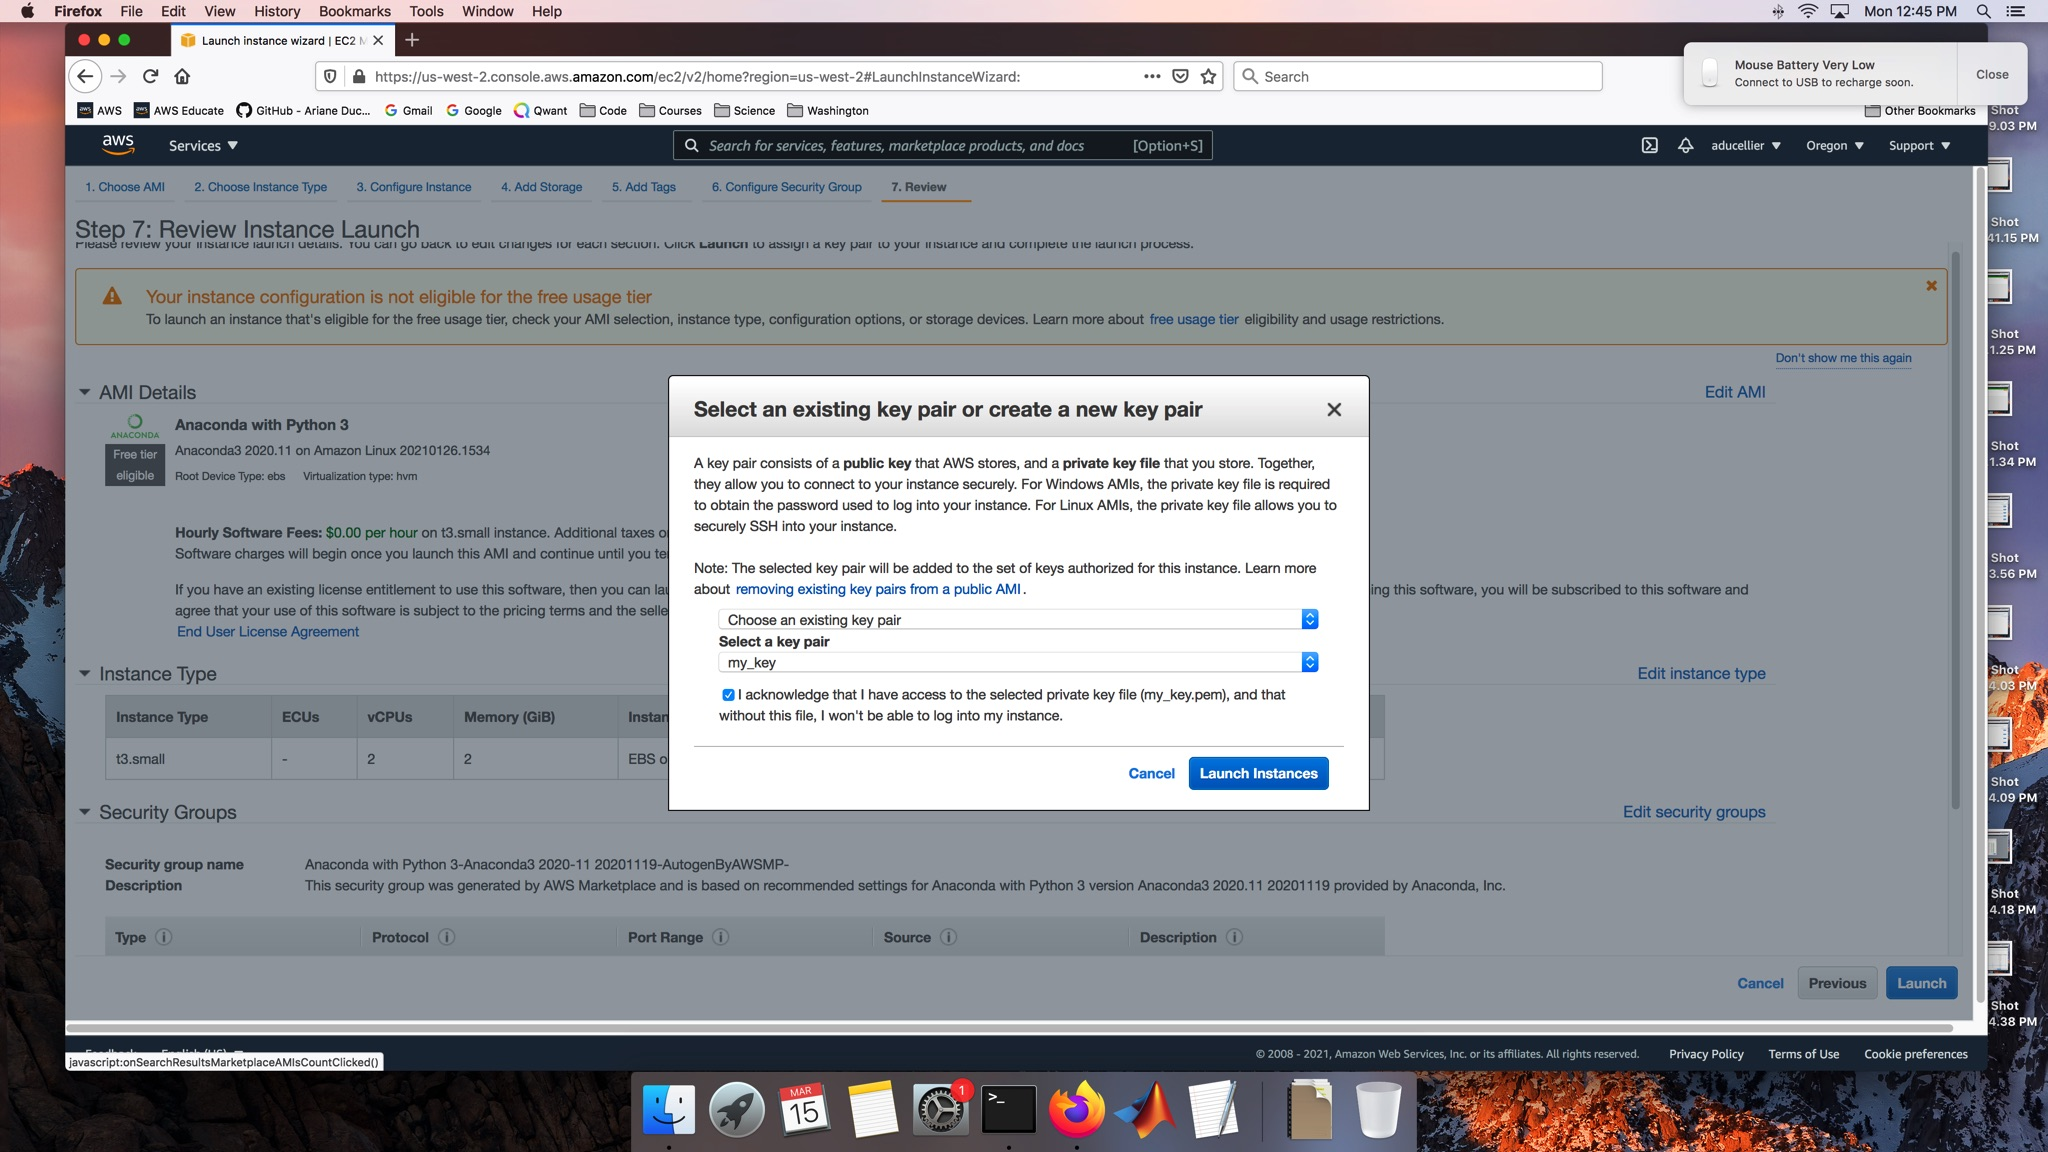
\includegraphics[width=11cm]{figures/choose_key_pair.jpg}};
		\draw<1>[red, thick] (3.8,2.5) rectangle ++(0.6,0.3);
		\draw<1>[red, thick] (6.3,1.9) rectangle ++(0.9,0.3);
	\end{tikzpicture}
	\end{frame}

	\begin{frame}
	\frametitle{Your EC2 instance is launching}
	\begin{tikzpicture}
		\node[anchor=south west, inner sep=0] at (0,0) {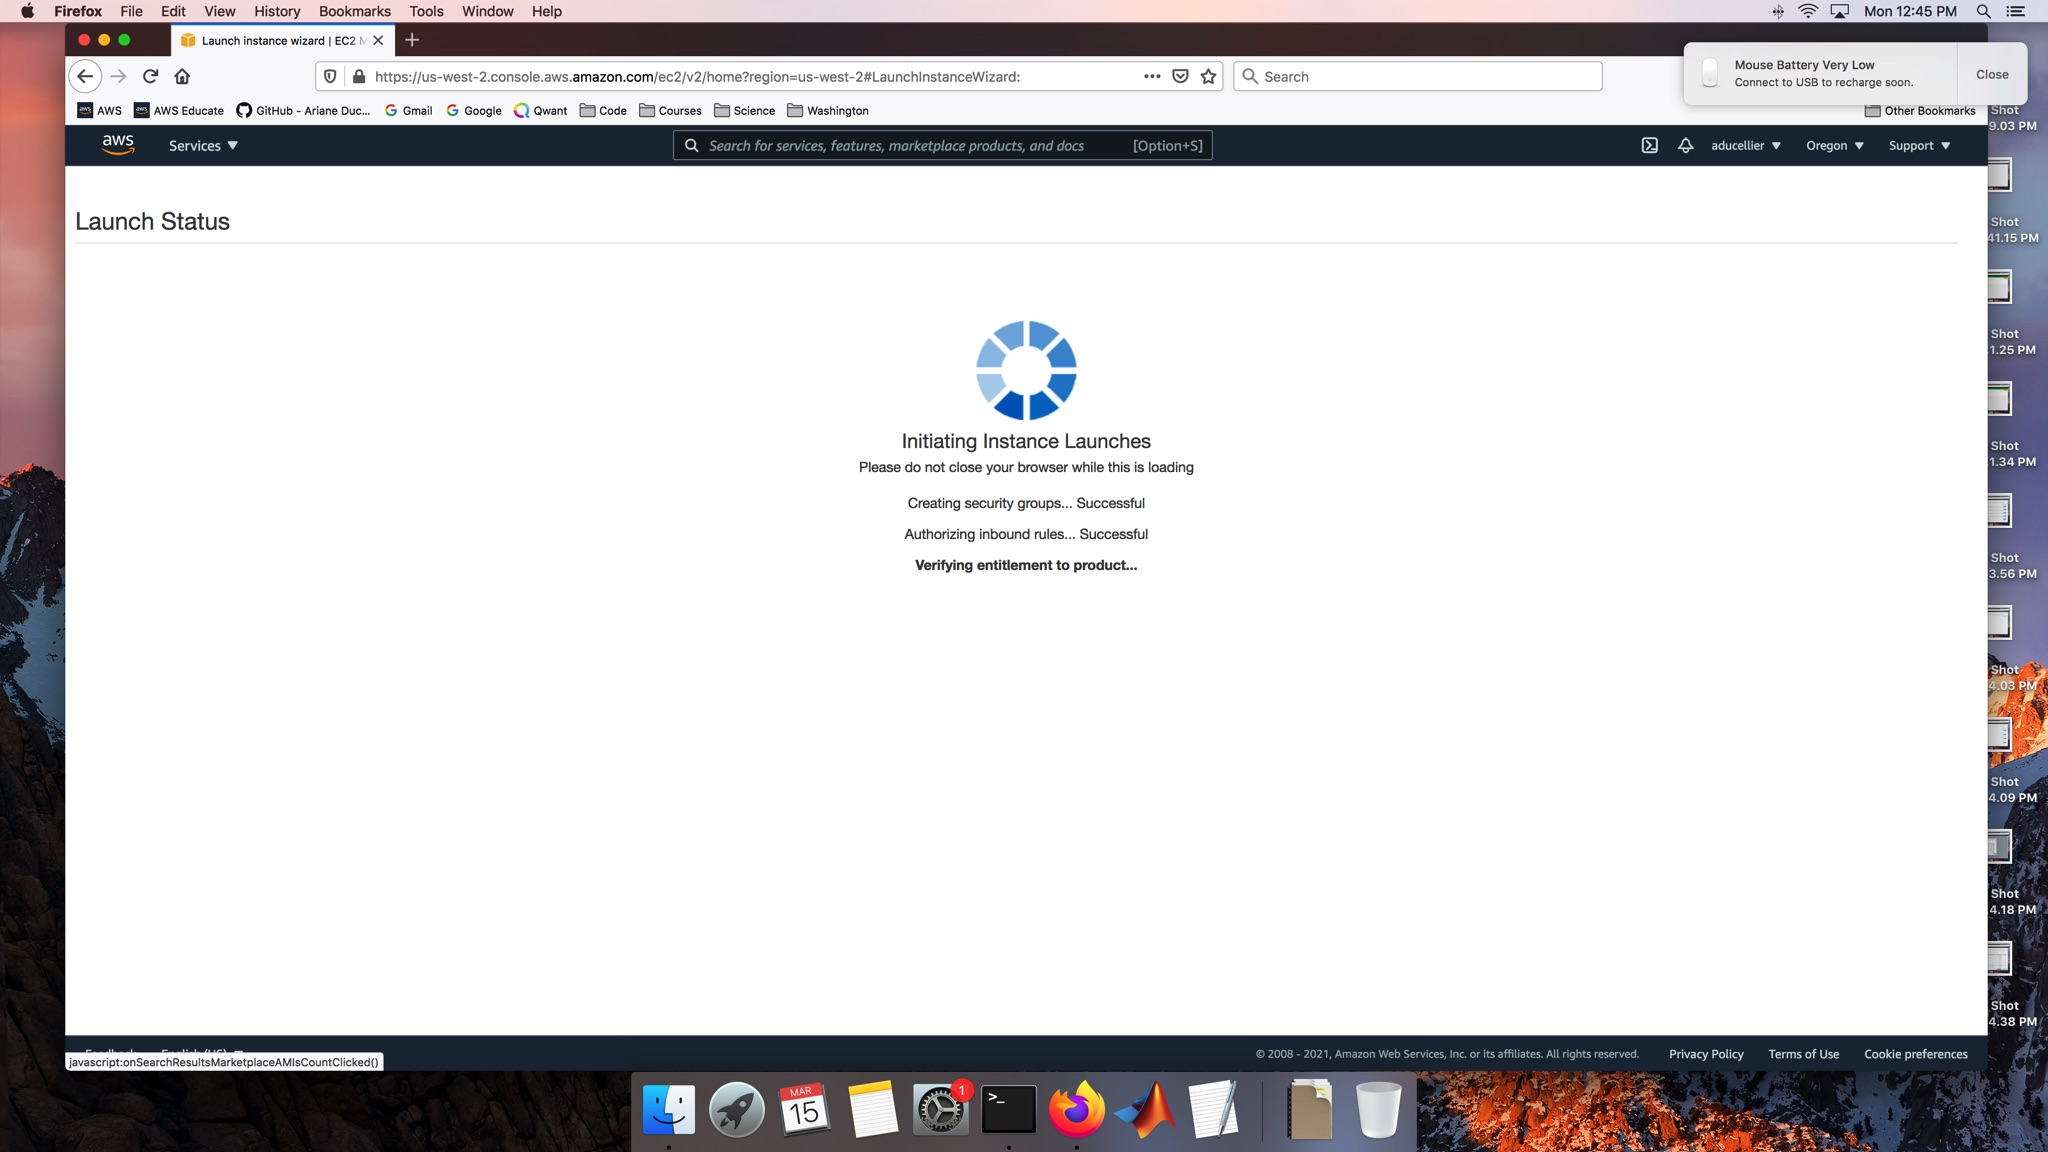
\includegraphics[width=11cm]{figures/ec2_is_starting.jpg}};
	\end{tikzpicture}
	\end{frame}

	\begin{frame}
	\frametitle{Go back to the list of instances}
	\begin{tikzpicture}
		\node[anchor=south west, inner sep=0] at (0,0) {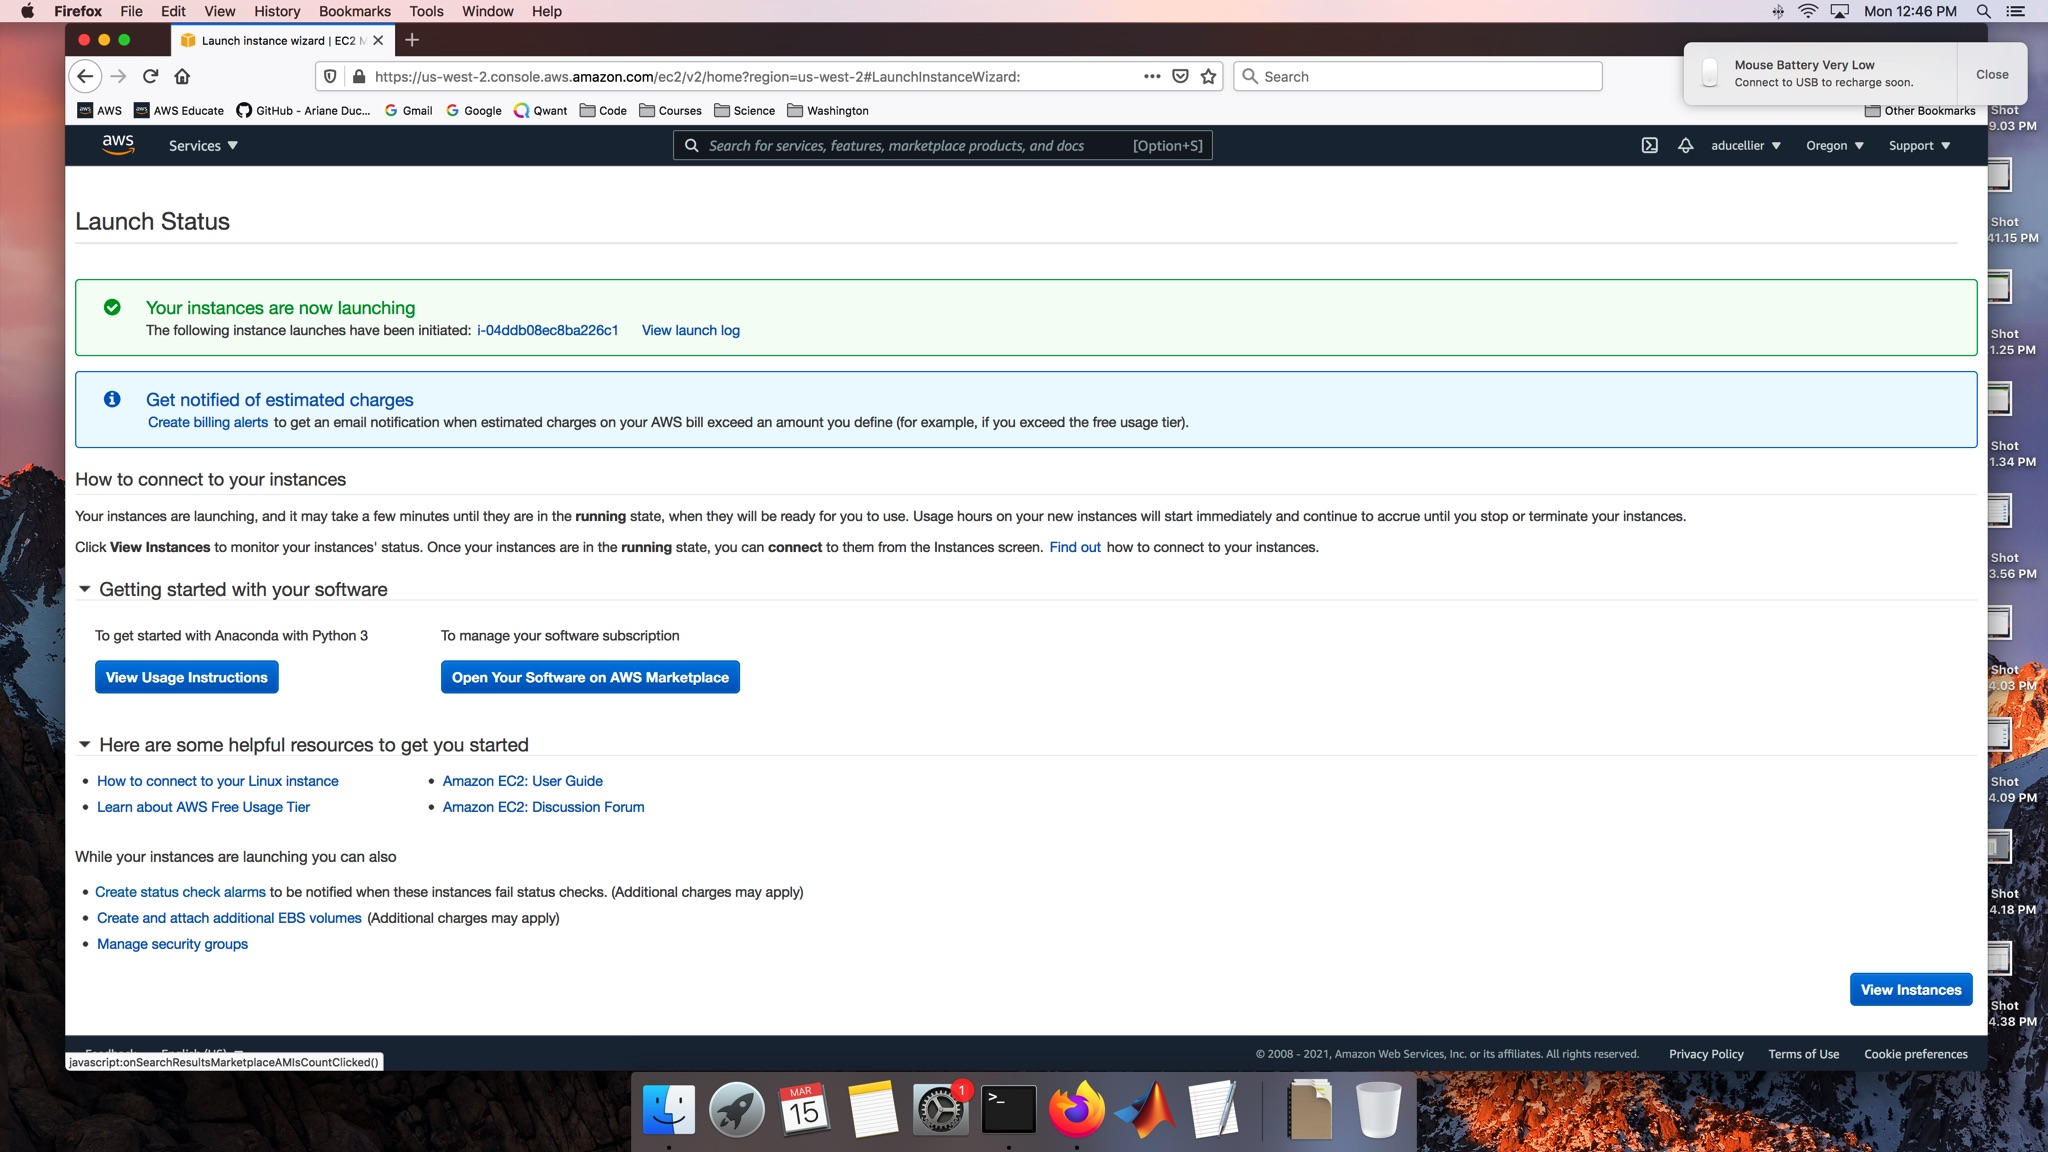
\includegraphics[width=11cm]{figures/go_back_to_instances.jpg}};
		\draw<1>[red, thick] (9.8,0.7) rectangle ++(0.9,0.3);
	\end{tikzpicture}
	\end{frame}

	\begin{frame}
	\frametitle{Your new EC2 instance is here}
	\begin{tikzpicture}
		\node[anchor=south west, inner sep=0] at (0,0) {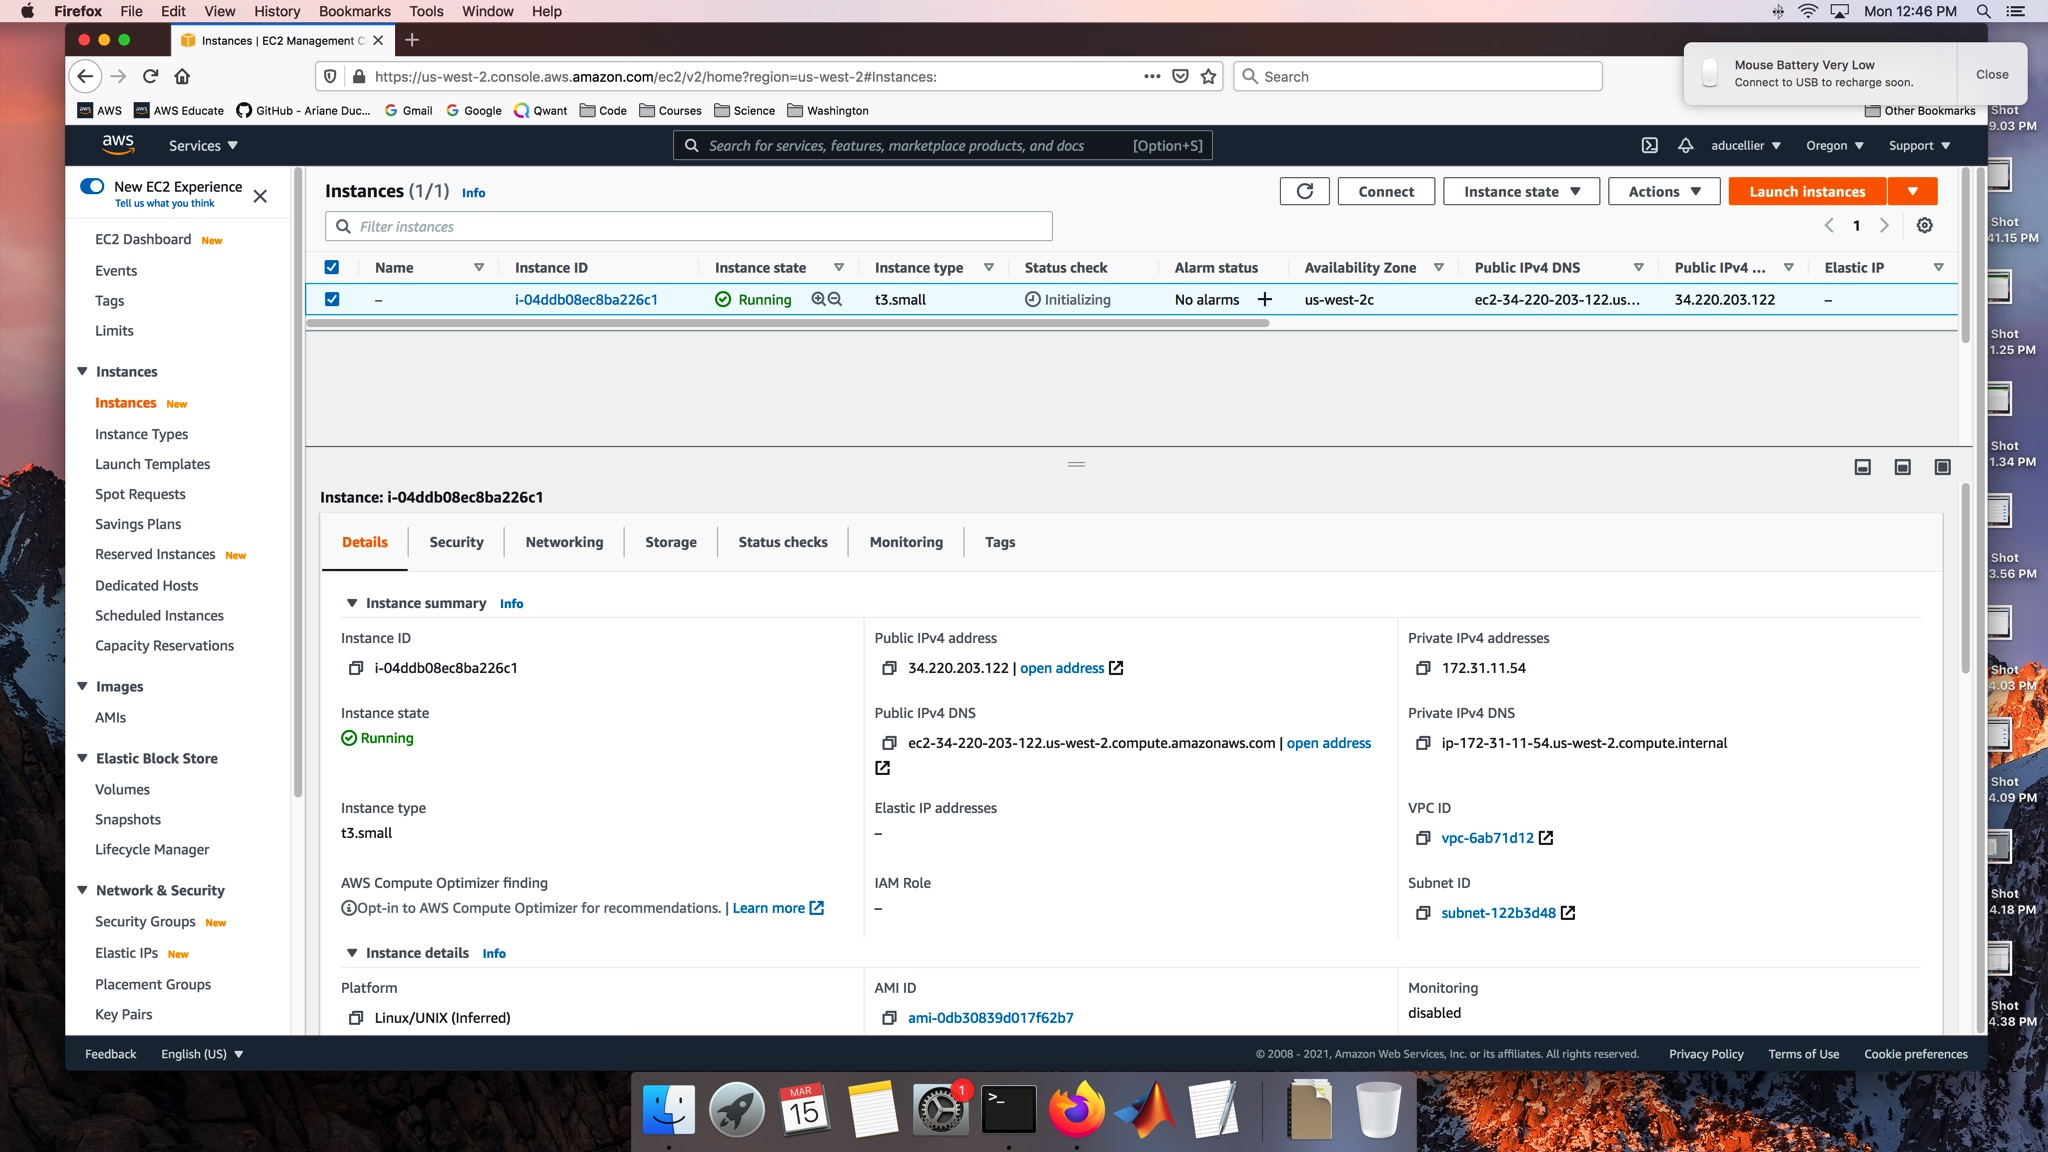
\includegraphics[width=11cm]{figures/ec2_is_here.jpg}};
		\draw<1>[red, thick] (1.6,4.4) rectangle ++(3.0,0.3);
	\end{tikzpicture}
	\end{frame}

	\begin{frame}
	\frametitle{You can modify the tags}
	\begin{tikzpicture}
		\node[anchor=south west, inner sep=0] at (0,0) {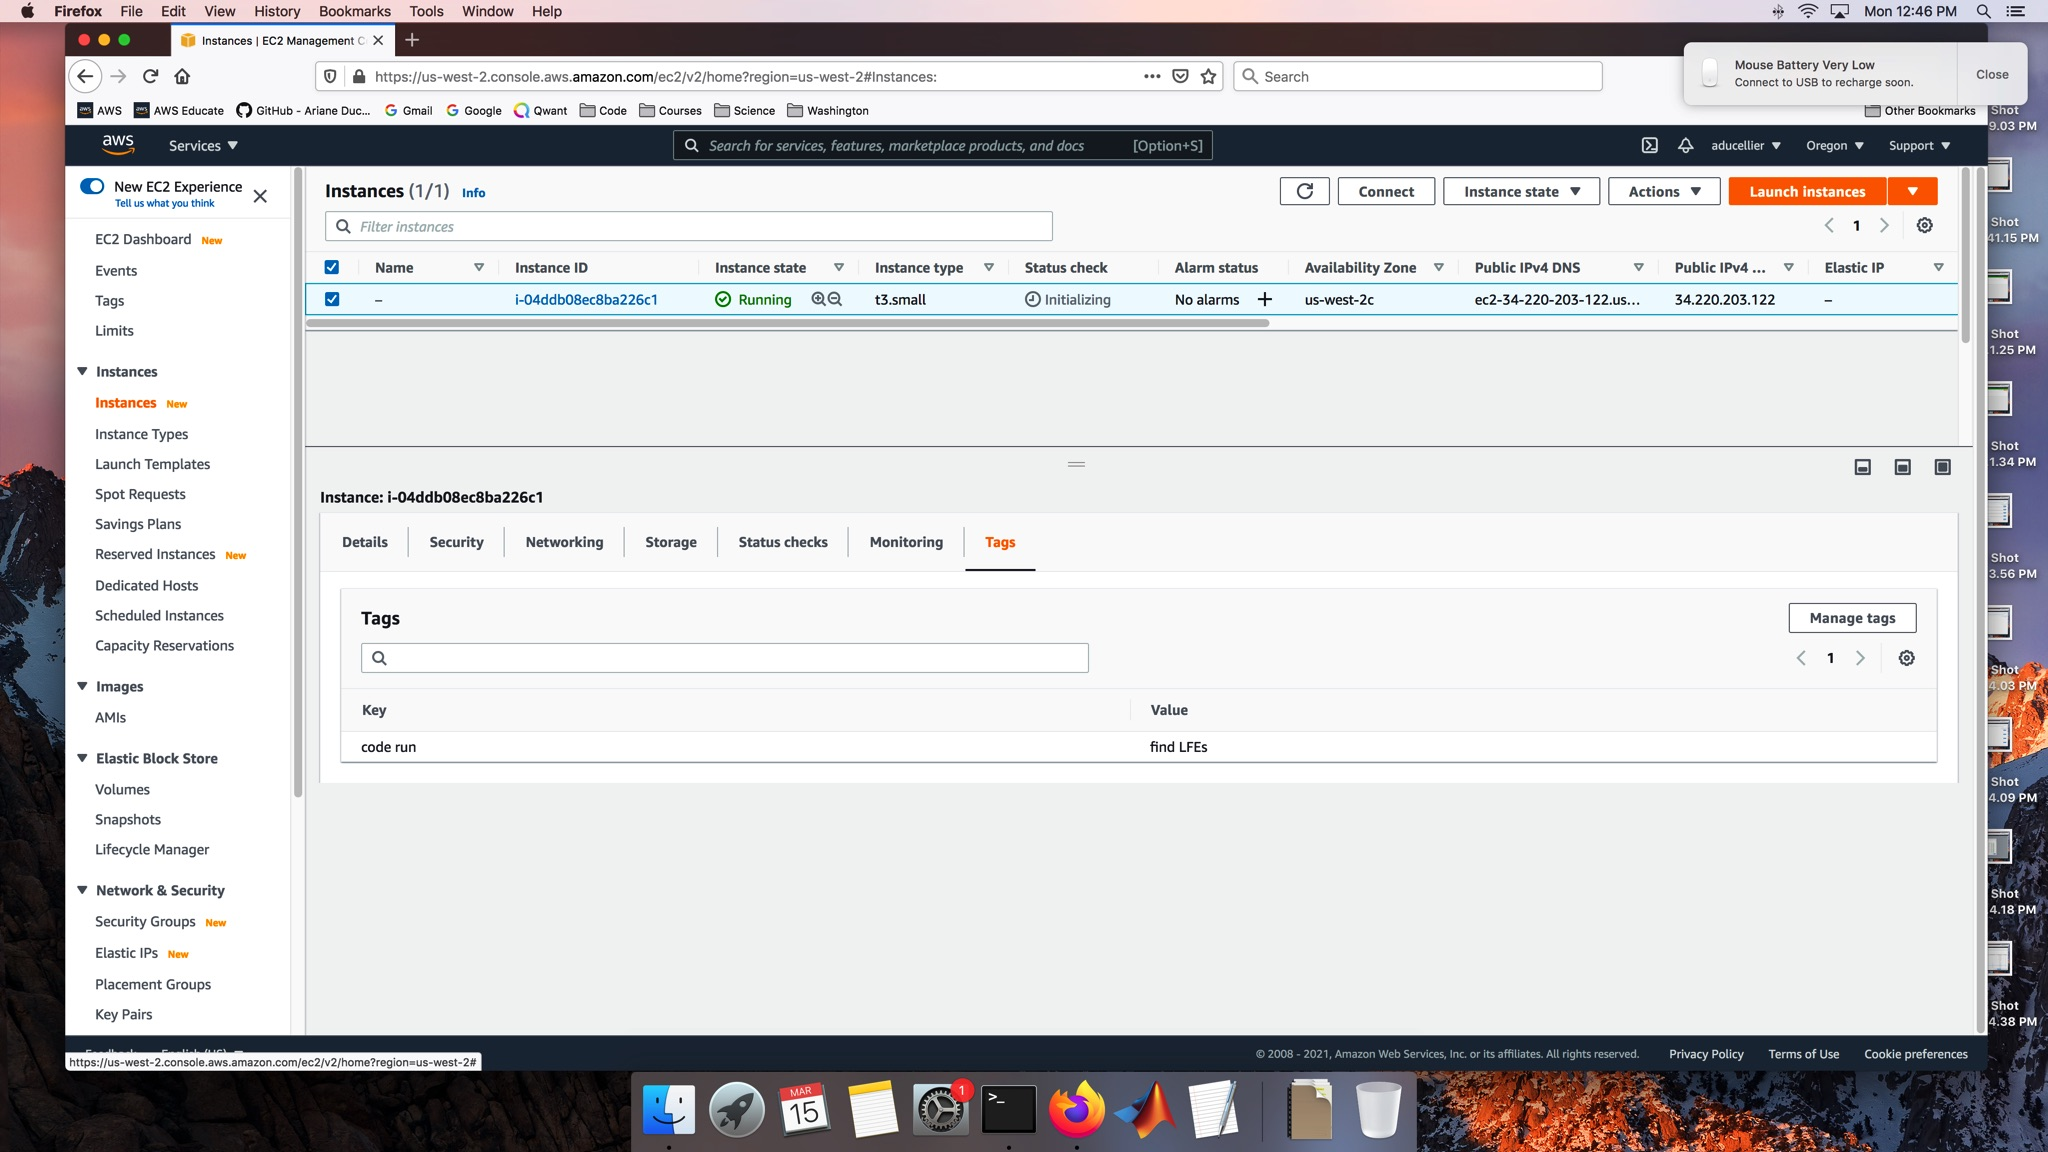
\includegraphics[width=11cm]{figures/change_tag.jpg}};
		\draw<1>[red, thick] (5.2,3.1) rectangle ++(0.4,0.3);
	\end{tikzpicture}
	\end{frame}

	\begin{frame}
	\frametitle{Your can modify the security group}
	\begin{tikzpicture}
		\node[anchor=south west, inner sep=0] at (0,0) {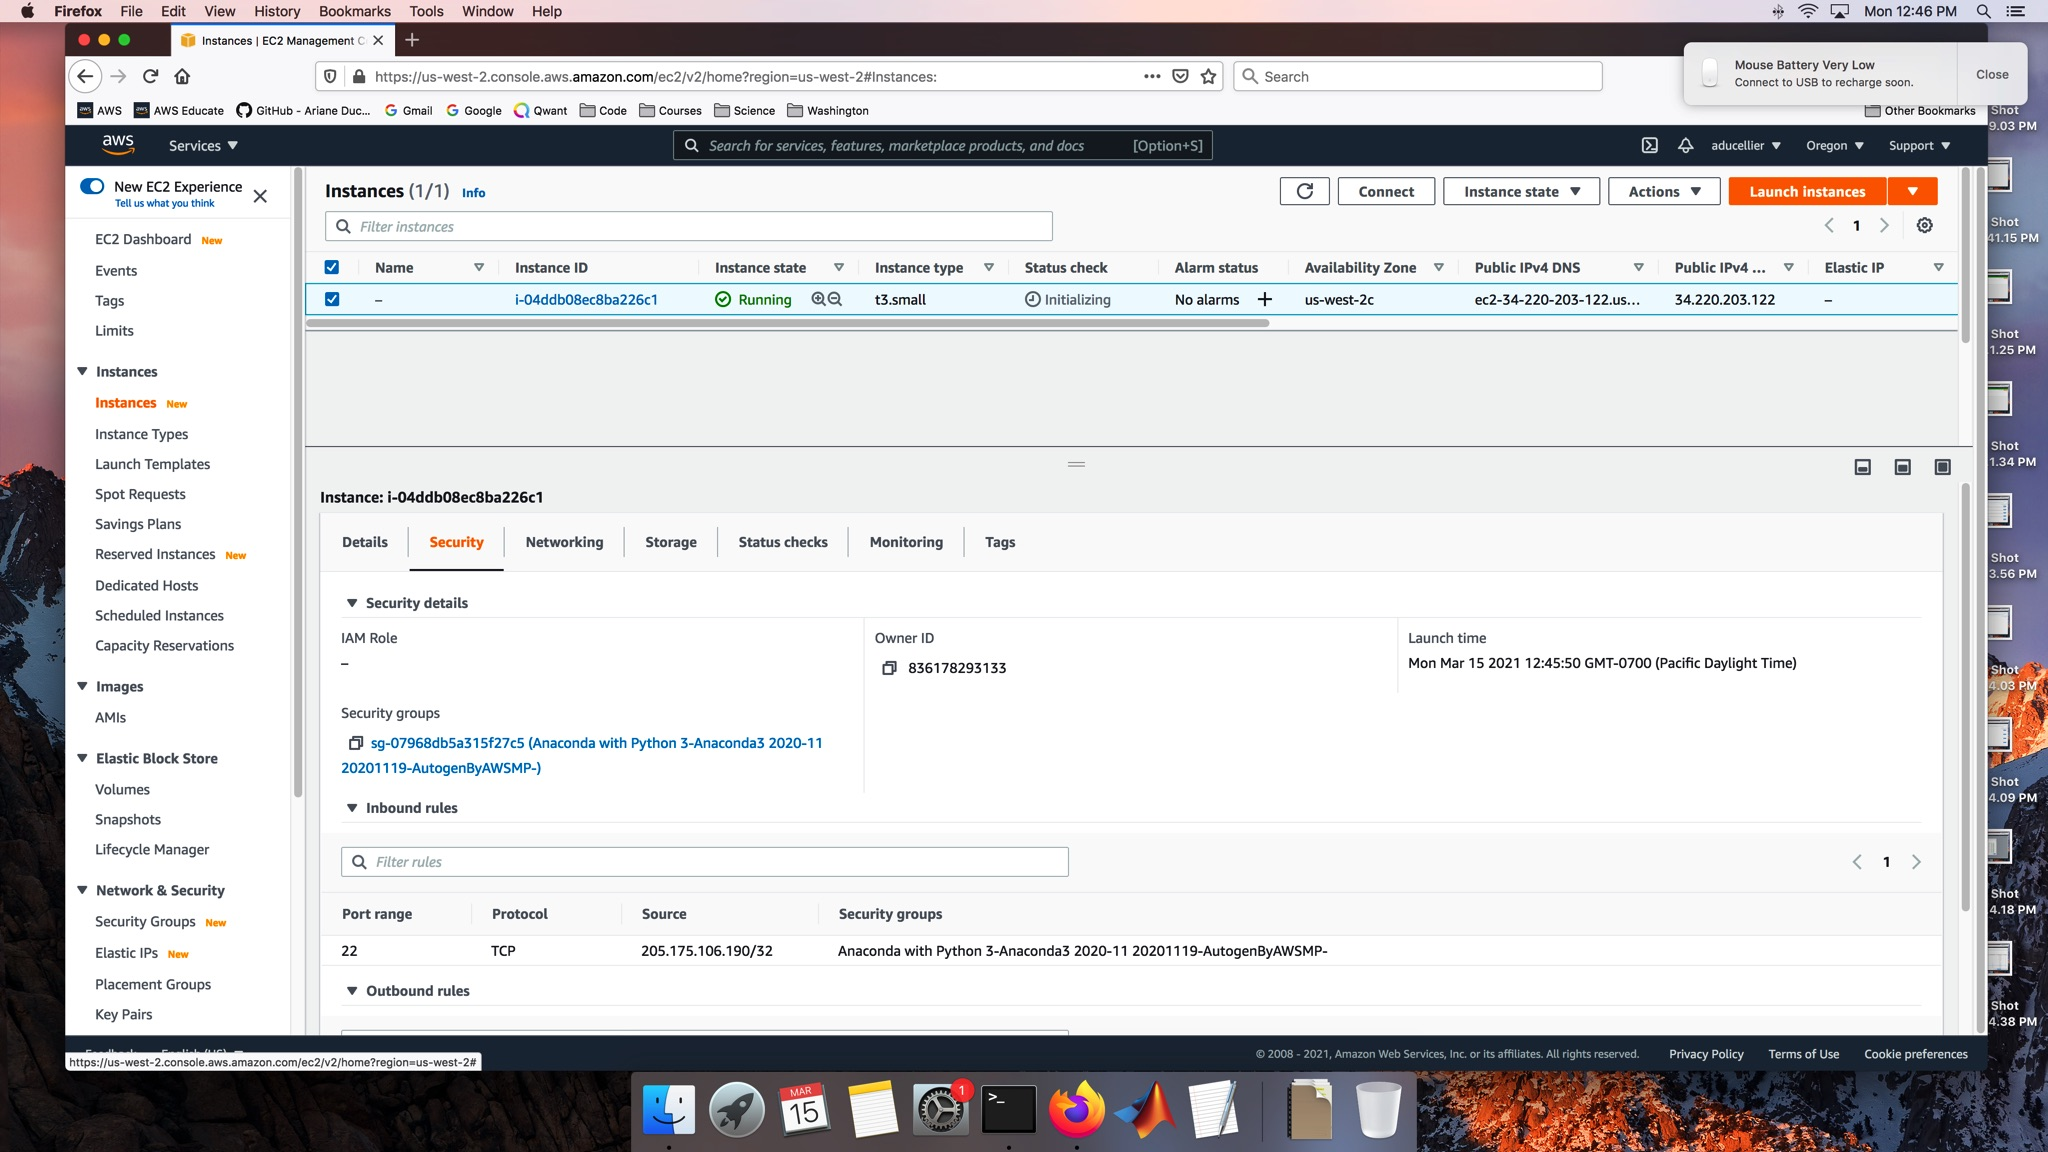
\includegraphics[width=11cm]{figures/change_security_group.jpg}};
		\draw<1>[red, thick] (2.2,3.1) rectangle ++(0.5,0.3);
		\draw<1>[red, thick] (1.8,1.9) rectangle ++(2.7,0.4);
	\end{tikzpicture}
	\end{frame}

	\begin{frame}
	\frametitle{Change the rules to connect to your instances}
	\begin{tikzpicture}
		\node[anchor=south west, inner sep=0] at (0,0) {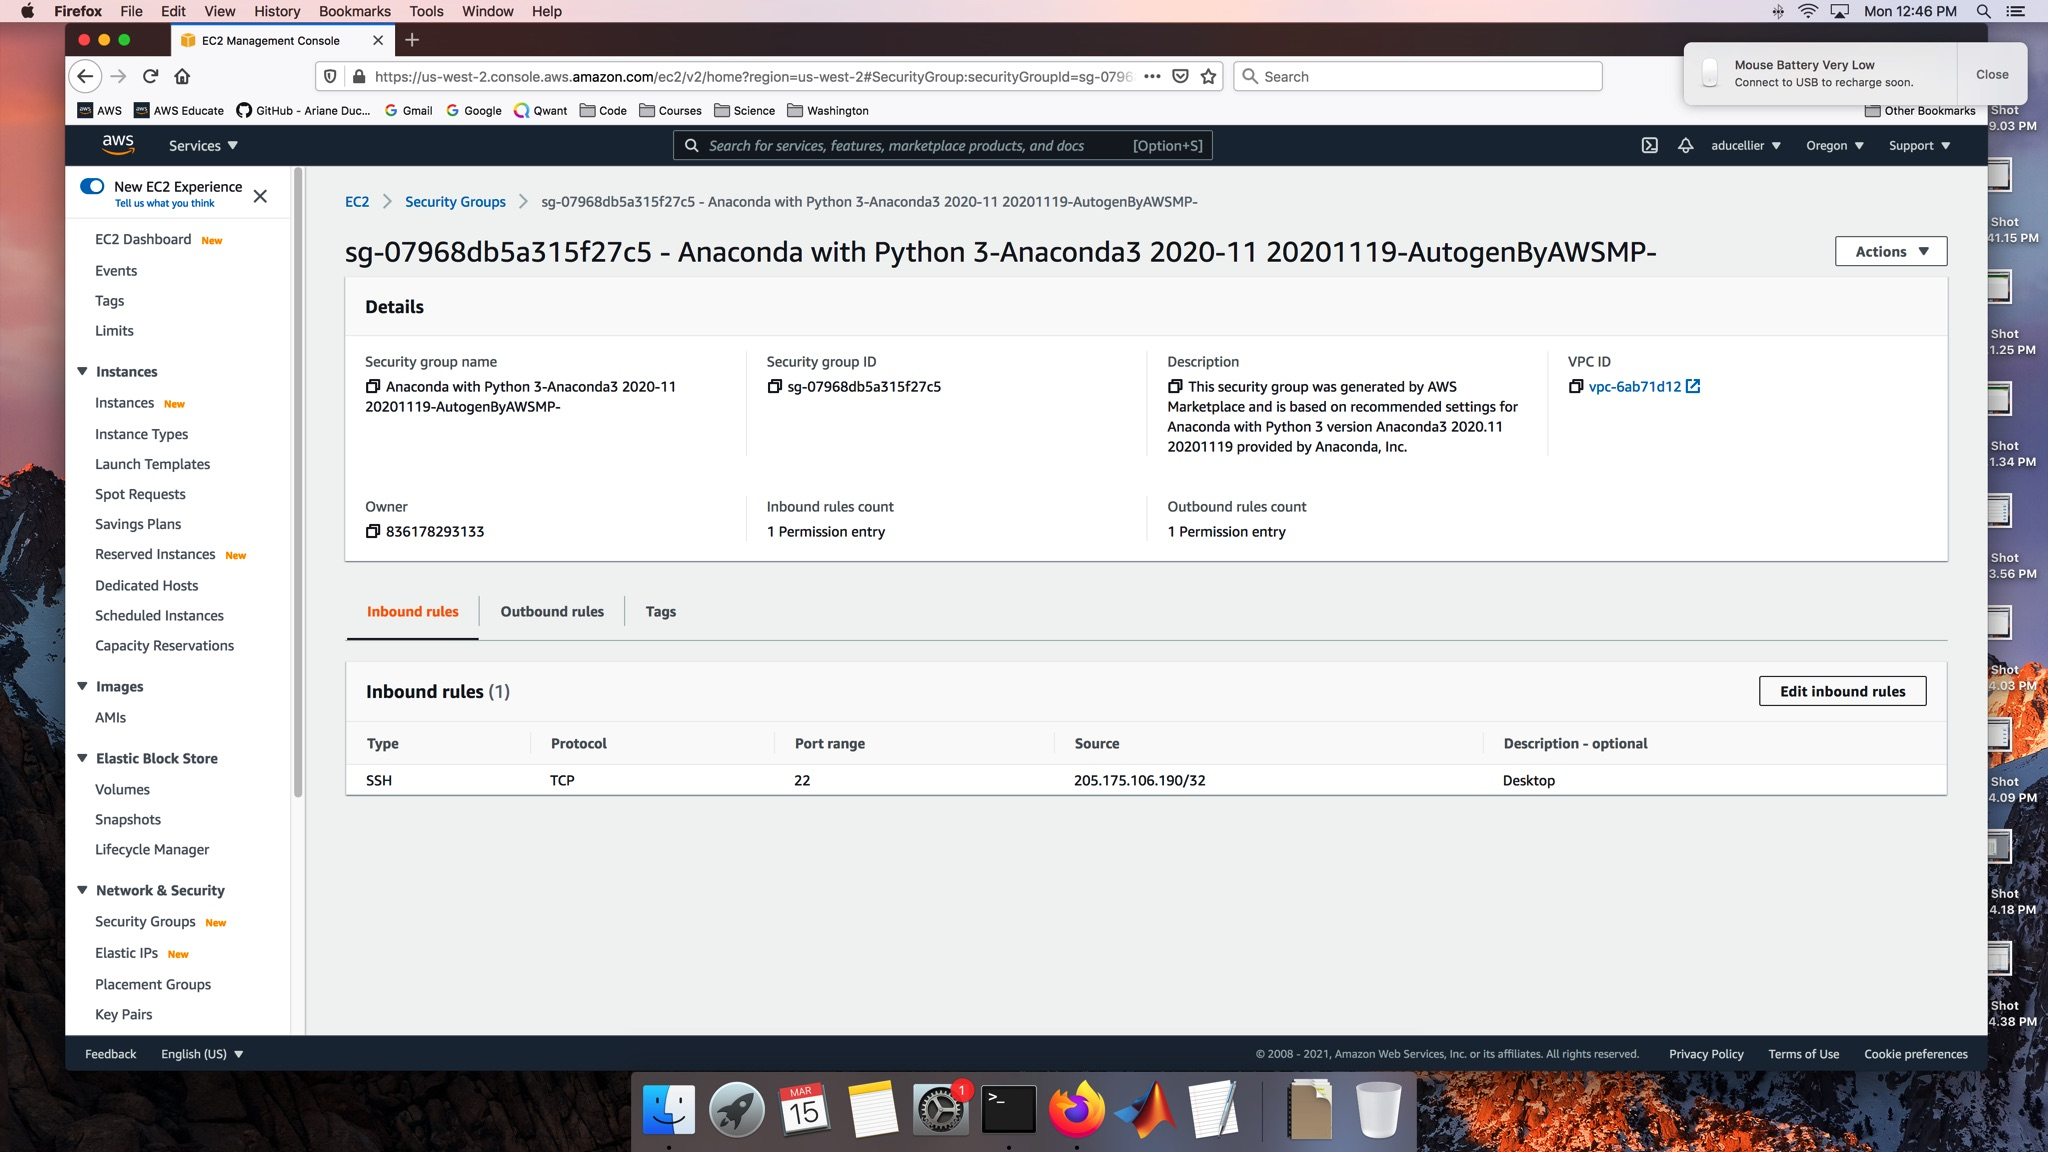
\includegraphics[width=11cm]{figures/add_security_rule.jpg}};
		\draw<1>[red, thick] (9.4,2.3) rectangle ++(1.0,0.3);
	\end{tikzpicture}
	\end{frame}

	\begin{frame}
	\frametitle{Your IP may have changed since the last time you connected}
	\begin{tikzpicture}
		\node[anchor=south west, inner sep=0] at (0,0) {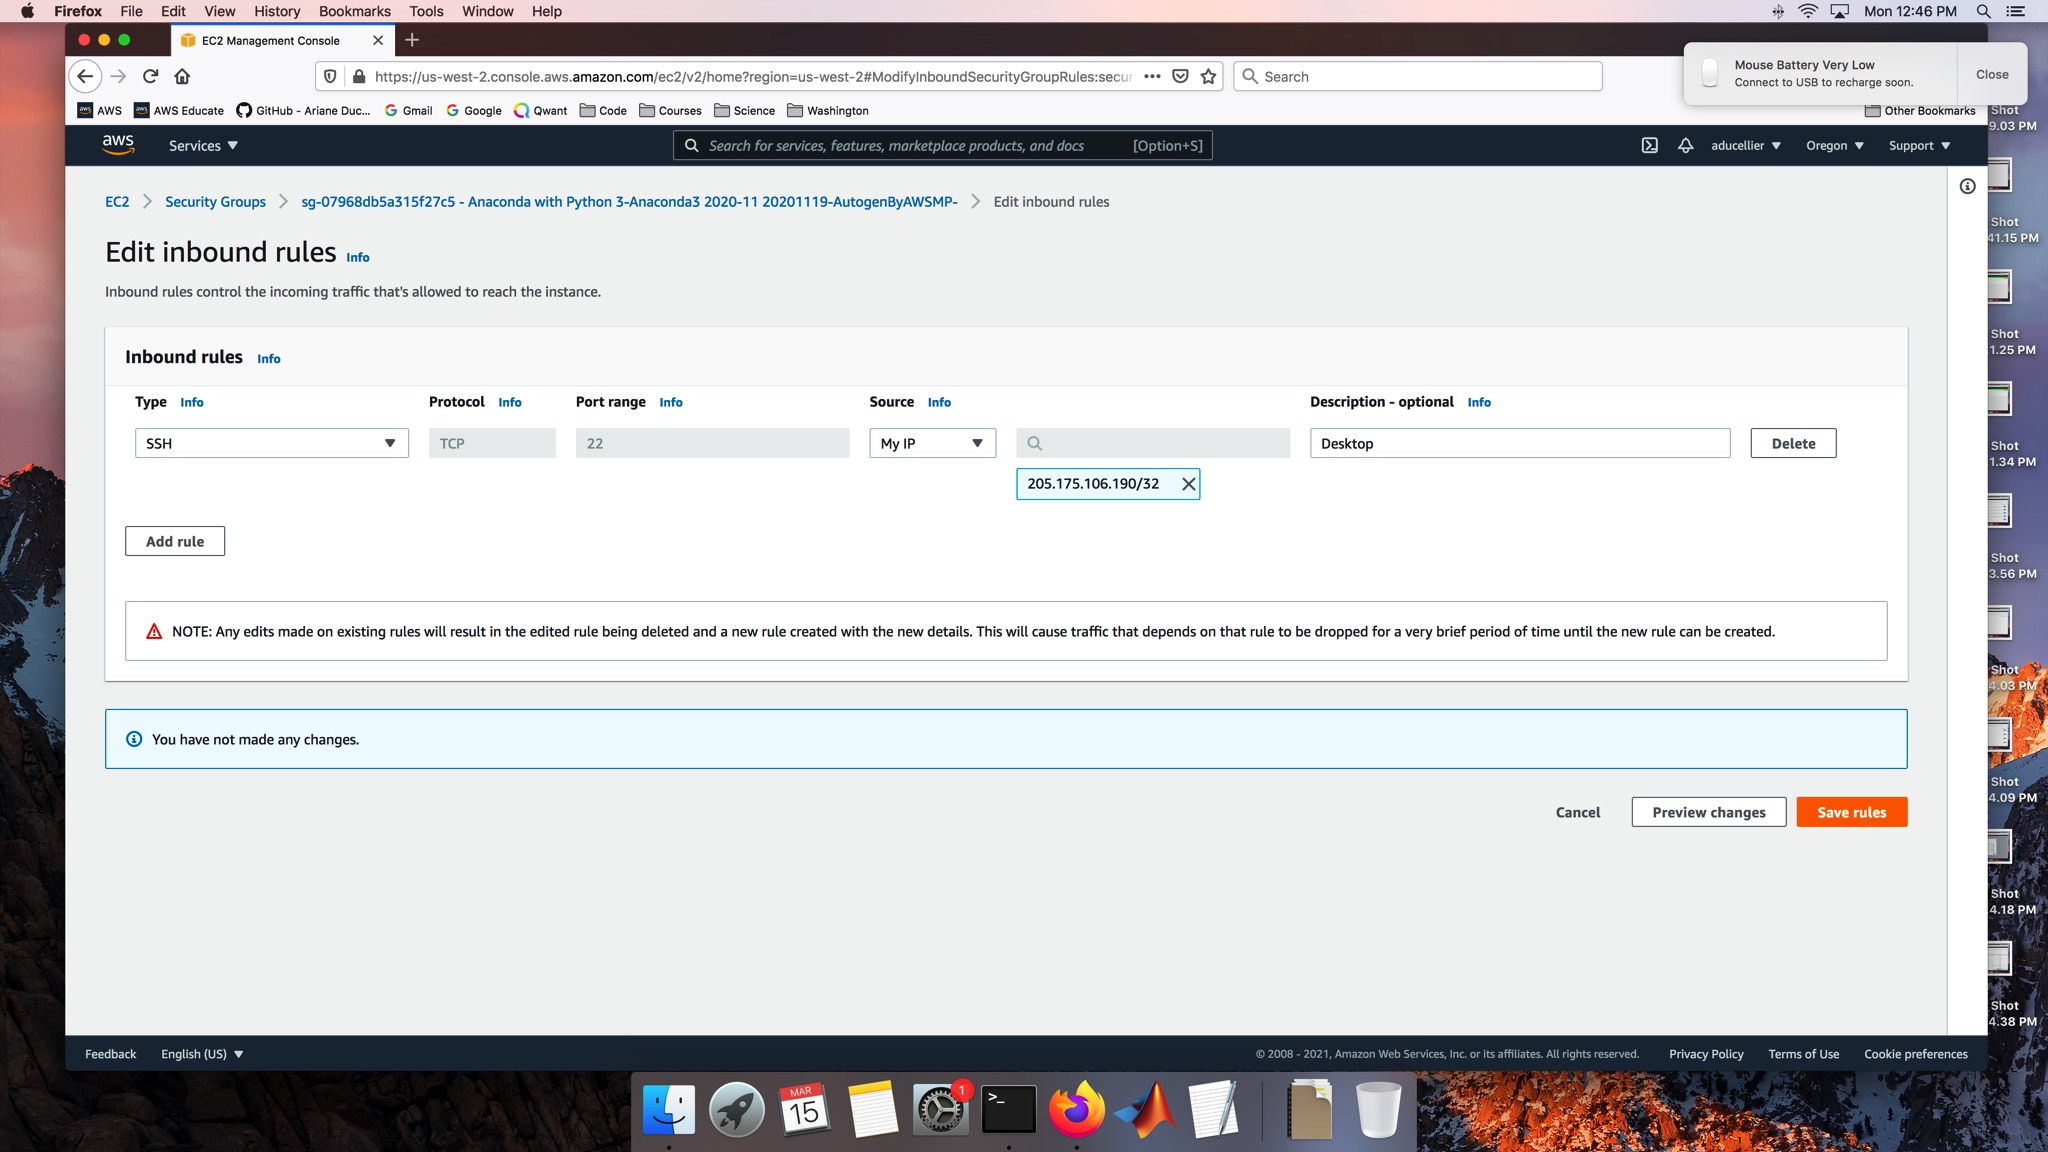
\includegraphics[width=11cm]{figures/modify_IP.jpg}};
		\draw<1>[red, thick] (4.6,3.7) rectangle ++(0.8,0.3);
		\draw<1>[red, thick] (9.6,1.7) rectangle ++(0.7,0.3);
	\end{tikzpicture}
	\end{frame}

	\begin{frame}
	\frametitle{Follow the instructions to connect with SSH}
	\begin{tikzpicture}
		\node[anchor=south west, inner sep=0] at (0,0) {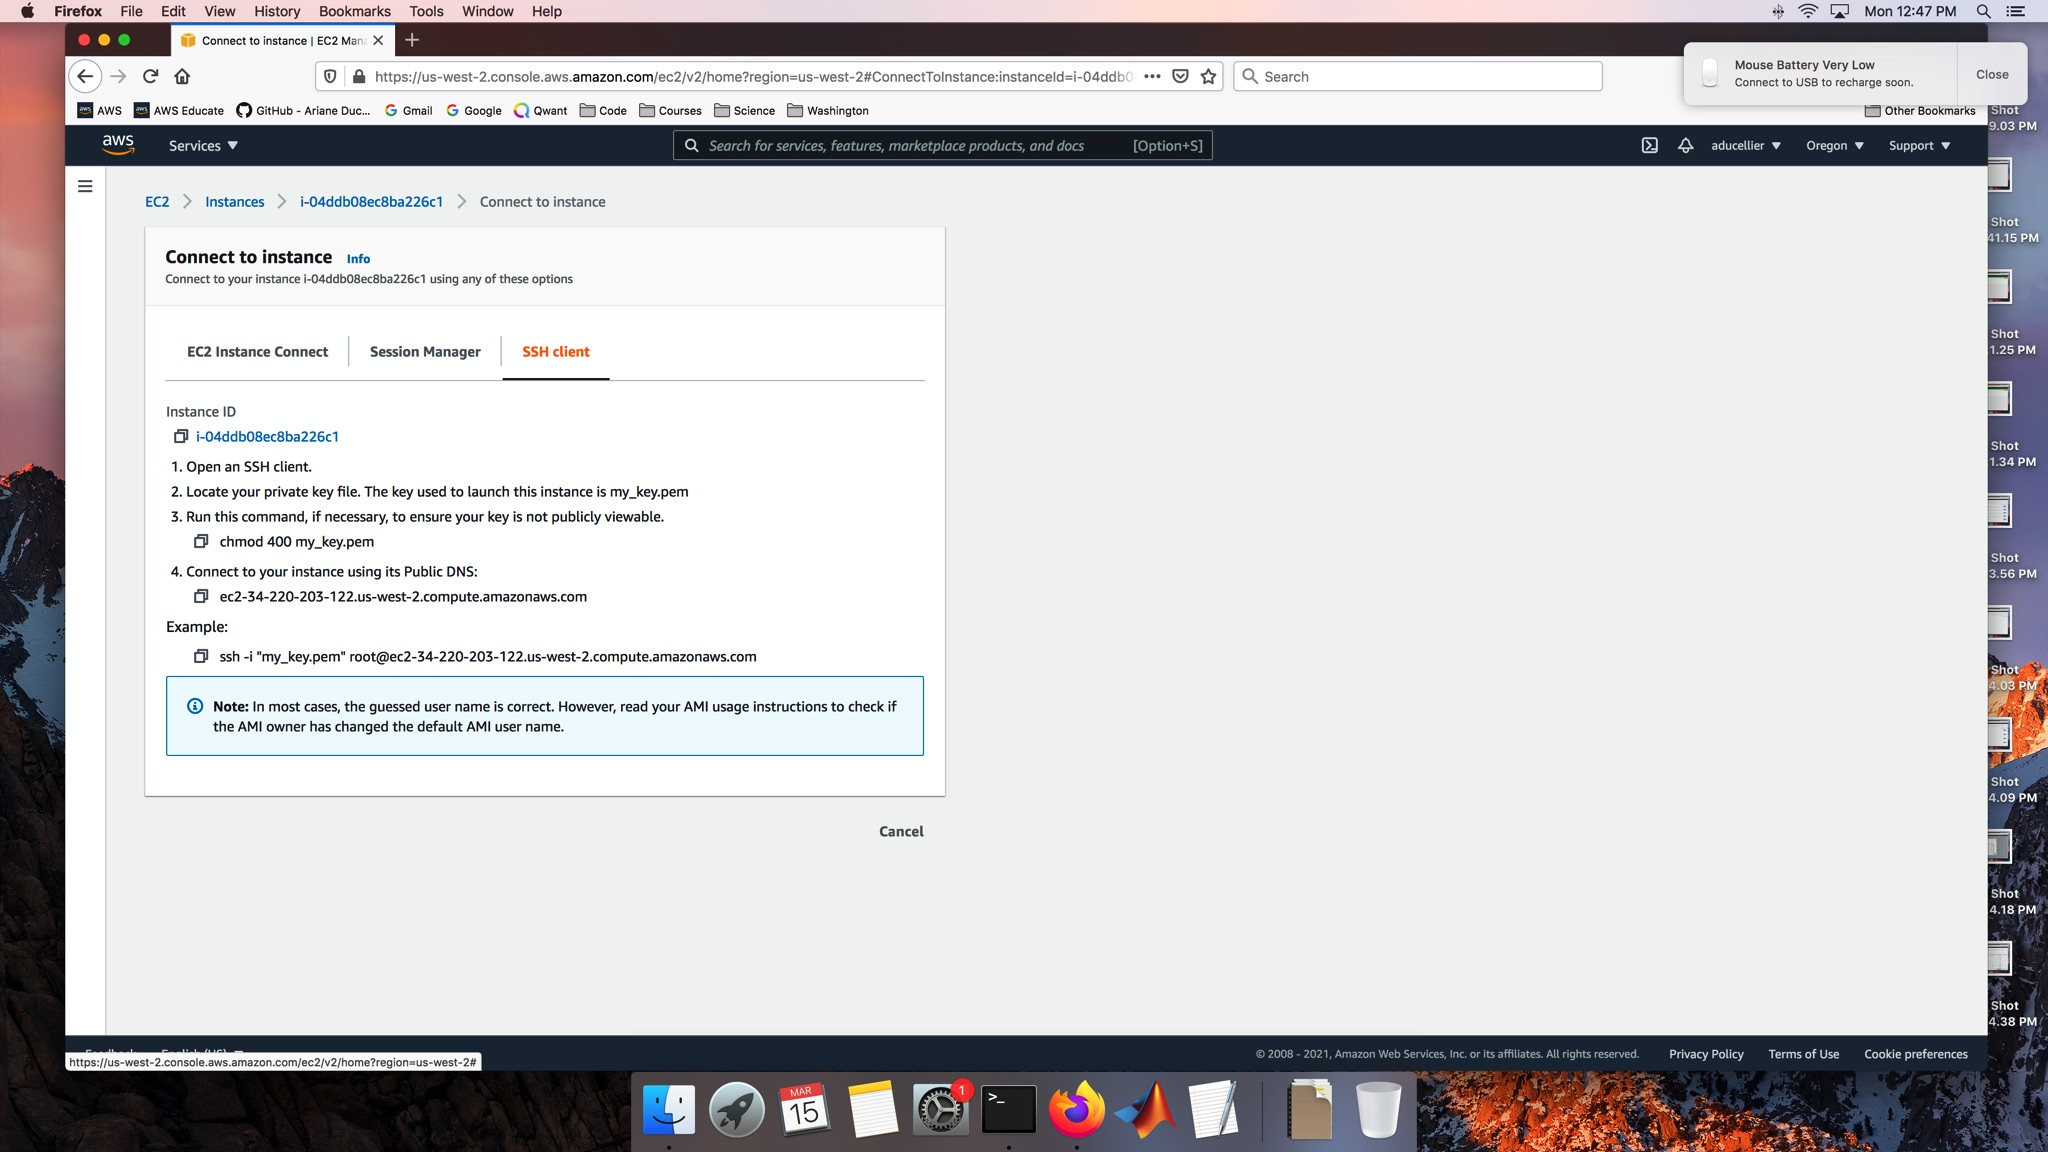
\includegraphics[width=11cm]{figures/open_terminal_and_connect.jpg}};
		\draw<1>[red, thick] (2.7,4.1) rectangle ++(0.6,0.3);
	\end{tikzpicture}
	\end{frame}

	\begin{frame}[fragile]
	\frametitle{Open an SSH terminal to connect to your instance}
	\begin{exampleblock}{}
		\begin{verbatim}
		> cd ~/.ssh
		> ssh -i "my_key.pem" ec2-user@ec2-XXX-XXX-XXX-XXX.
		us-west-2.compute.amazonaws.com
		\end{verbatim}
	\end{exampleblock}
	\end{frame}

	\begin{frame}[fragile]
	\frametitle{Install git and clone your repository}
	\begin{exampleblock}{}
		\begin{verbatim}
		> sudo yum install git
		> git clone "https://github.com/ArianeDucellier/
		catalog.git"
		\end{verbatim}
	\end{exampleblock}
	\end{frame}

	\begin{frame}[fragile]
	\frametitle{Create your Anaconda environment}
	\begin{exampleblock}{}
		\begin{verbatim}
		> cd catalog
		> conda env create -f environment.yml
		> conda activate catalog
		\end{verbatim}
	\end{exampleblock}
	\end{frame}

	\begin{frame}[fragile]
	\frametitle{In my case, I just prepare some input files}
	\begin{exampleblock}{}
		\begin{verbatim}
		> mkdir data/response
		> cd src
		> python get_responses.py
		\end{verbatim}
	\end{exampleblock}
	\end{frame}

	\begin{frame}[fragile]
	\frametitle{Use nohup to continue your computation after you disconnect}
	\begin{exampleblock}{}
		\begin{verbatim}
		> nohup python find_all_LFEs_parallel.py &
		> ps -x -o pid,user,%mem,command
		> exit
		\end{verbatim}
	\end{exampleblock}
	\end{frame}

	\begin{frame}
	\frametitle{Never forget to terminate your instances!!!}
	\begin{tikzpicture}
		\node[anchor=south west, inner sep=0] at (0,0) {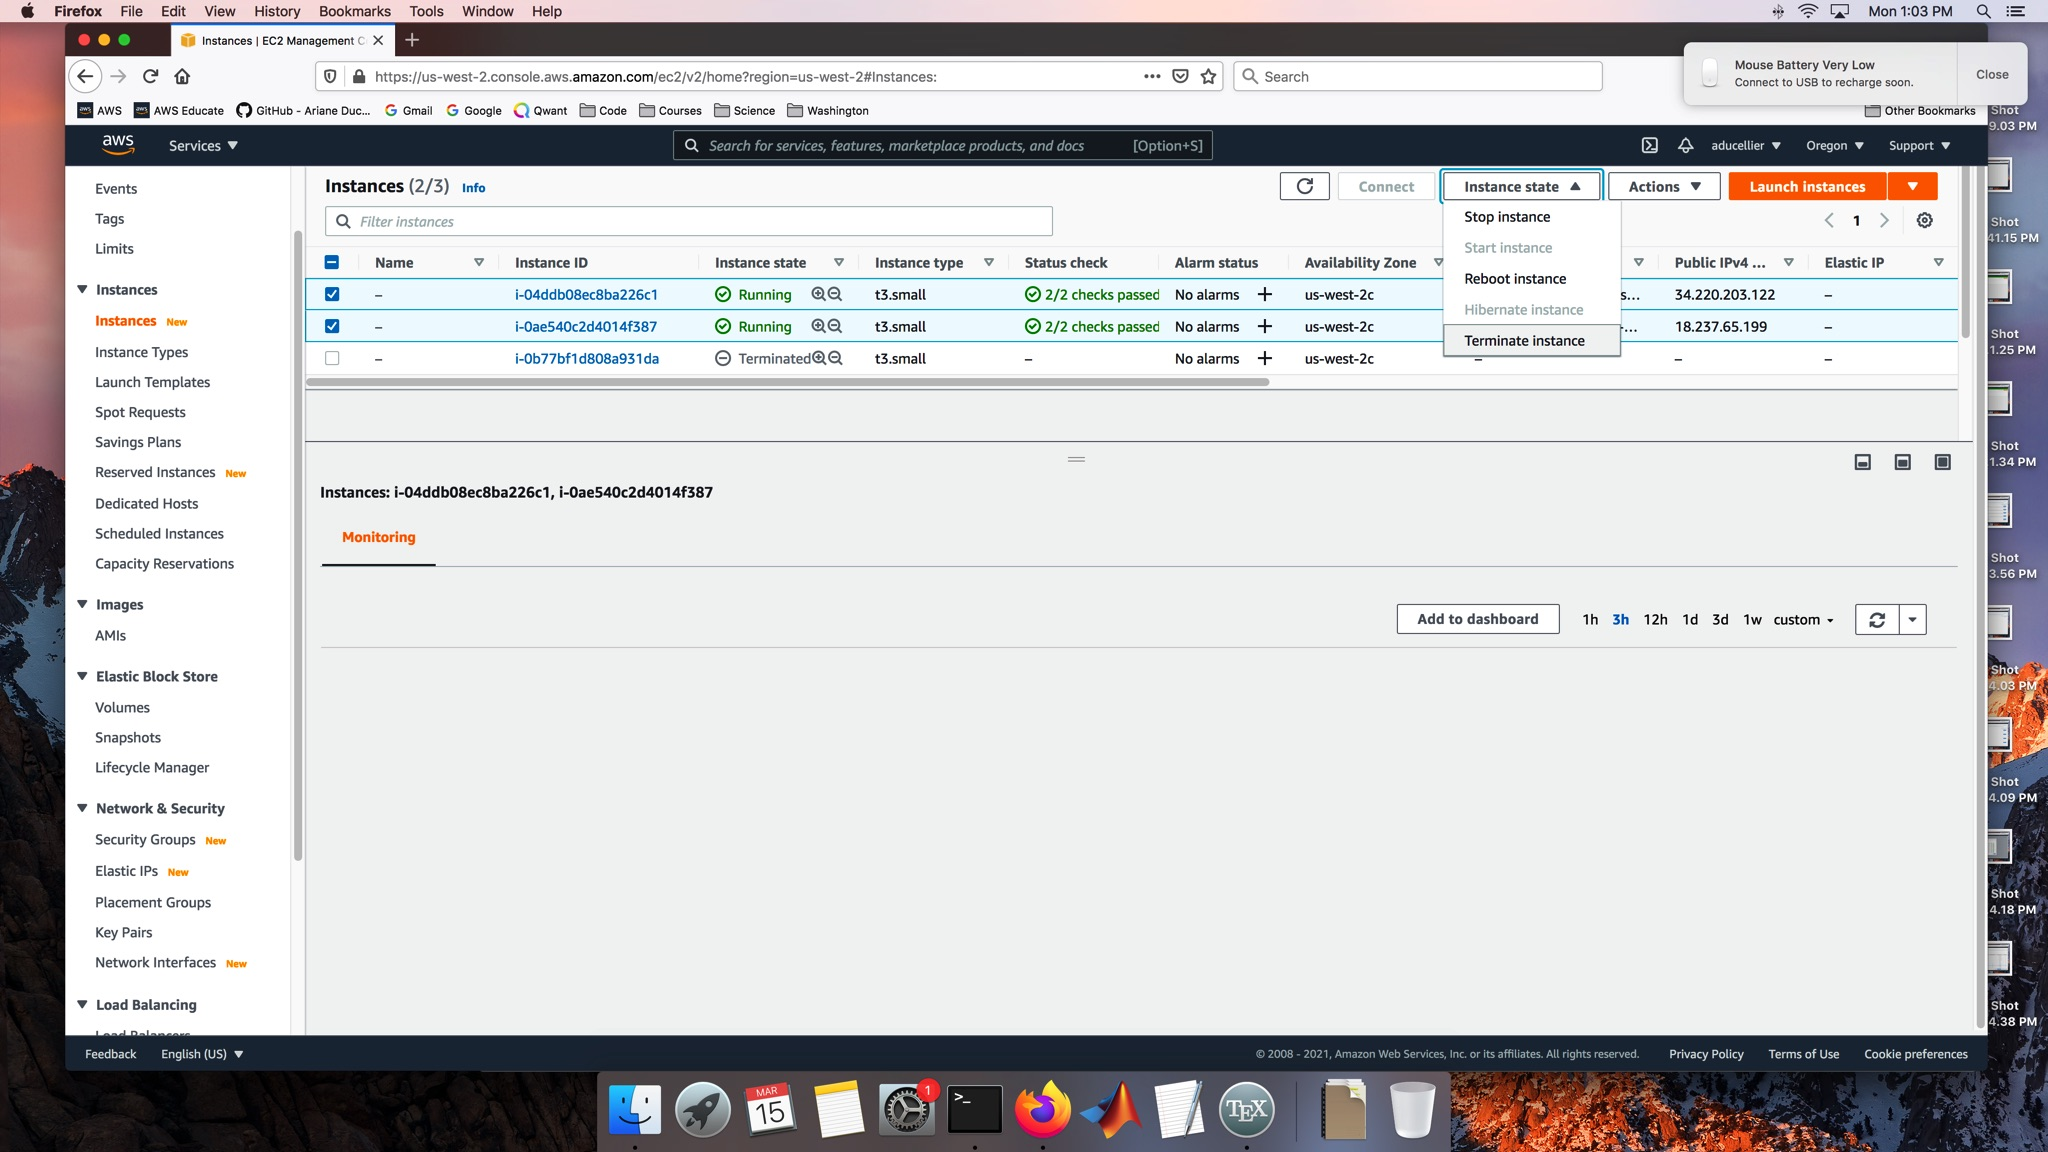
\includegraphics[width=11cm]{figures/do_not_forget_terminate.jpg}};
		\draw<1>[red, thick] (7.7,4.2) rectangle ++(1.0,0.3);
	\end{tikzpicture}
	\end{frame}

	\begin{frame}
	\frametitle{Never forget to terminate your instances!!!}
	\begin{tikzpicture}
		\node[anchor=south west, inner sep=0] at (0,0) {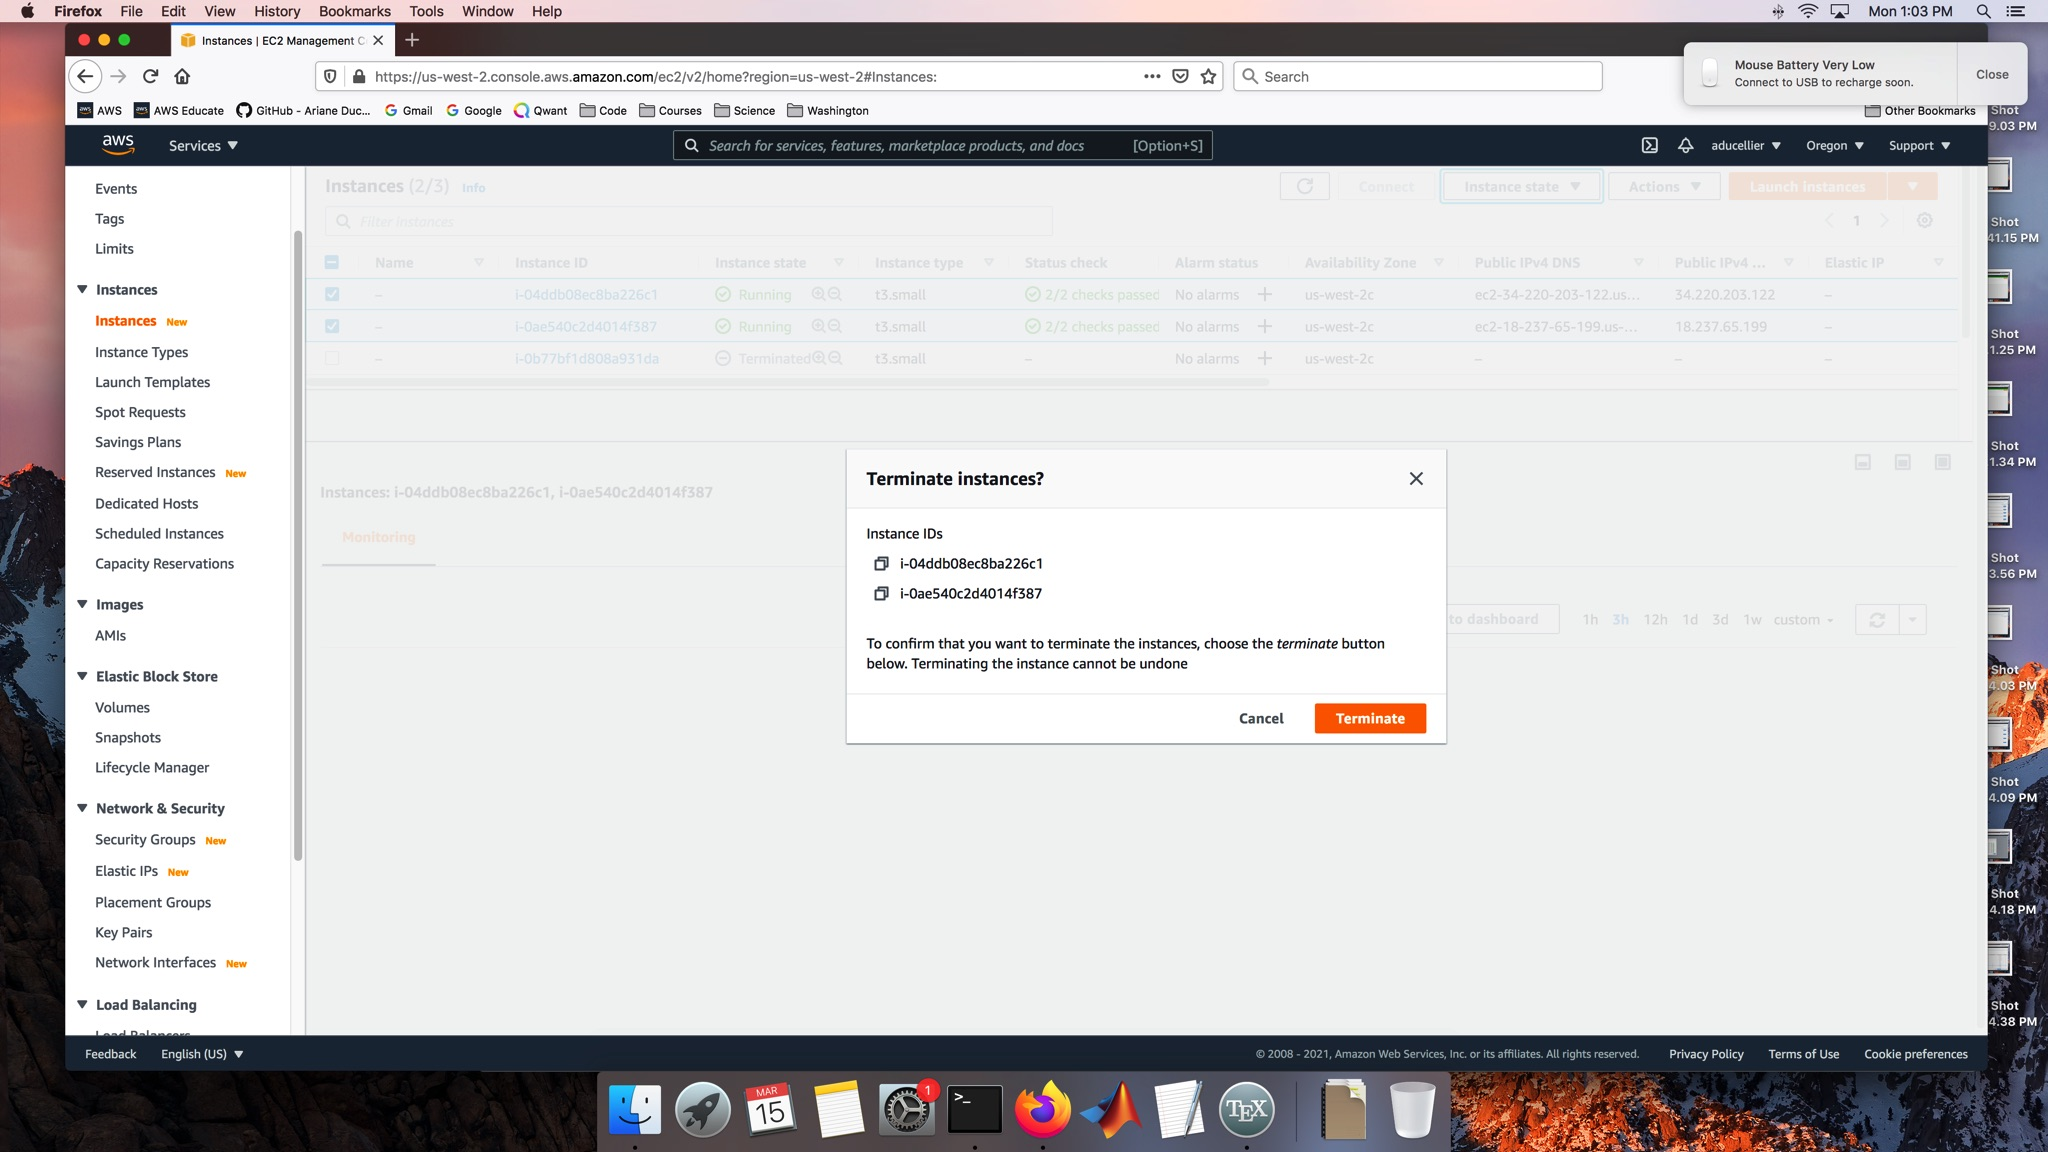
\includegraphics[width=11cm]{figures/terminate_instance.jpg}};
		\draw<1>[red, thick] (7.0,2.2) rectangle ++(0.7,0.3);
	\end{tikzpicture}
	\end{frame}

	\begin{frame}
	\frametitle{Check if your instance has been terminated}
	\begin{tikzpicture}
		\node[anchor=south west, inner sep=0] at (0,0) {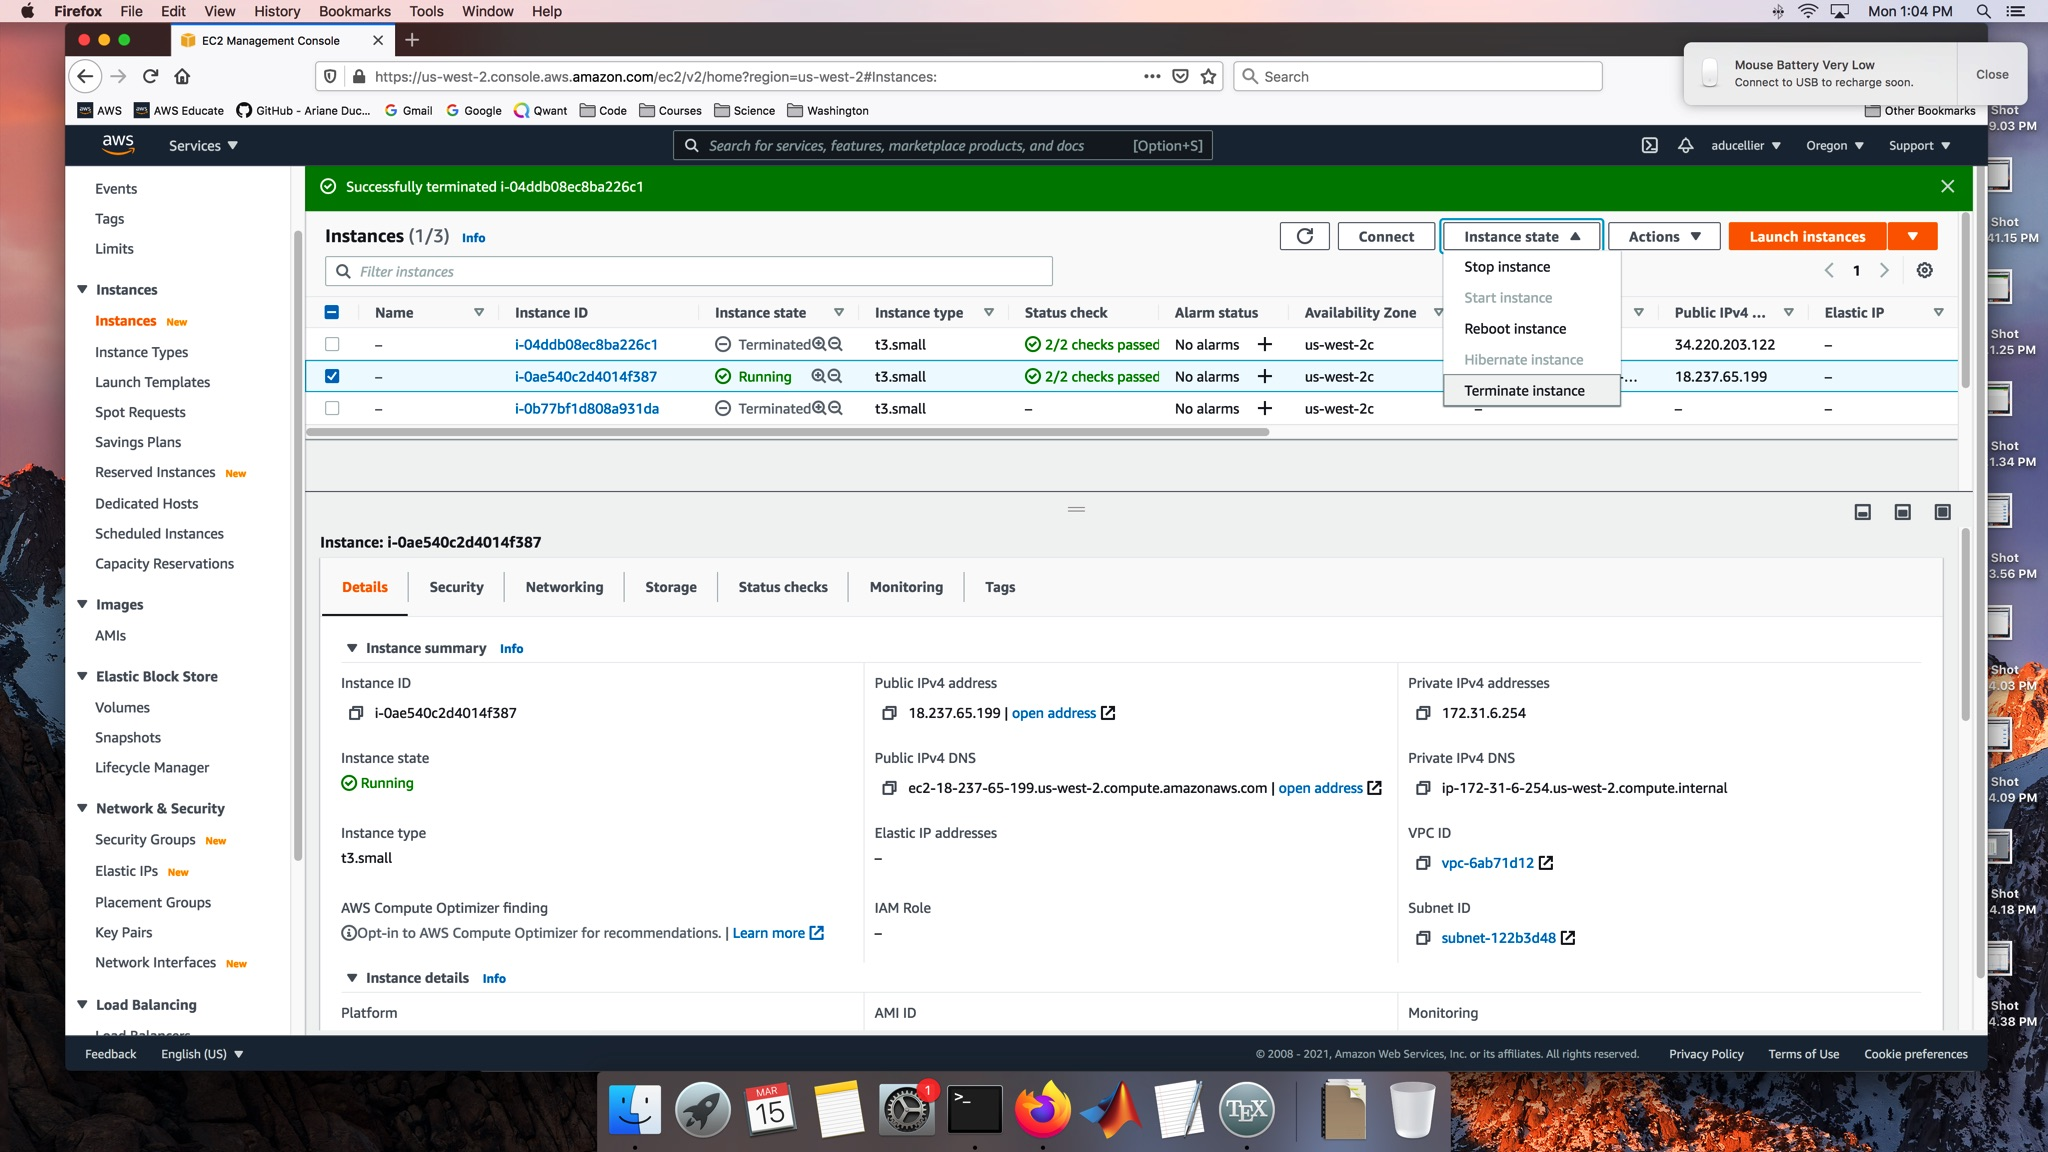
\includegraphics[width=11cm]{figures/check_terminated.jpg}};
		\draw<1>[red, thick] (3.8,4.2) rectangle ++(0.7,0.3);
	\end{tikzpicture}
	\end{frame}

	\begin{frame}
	\frametitle{Go to your billing dashboard}
	\begin{tikzpicture}
		\node[anchor=south west, inner sep=0] at (0,0) {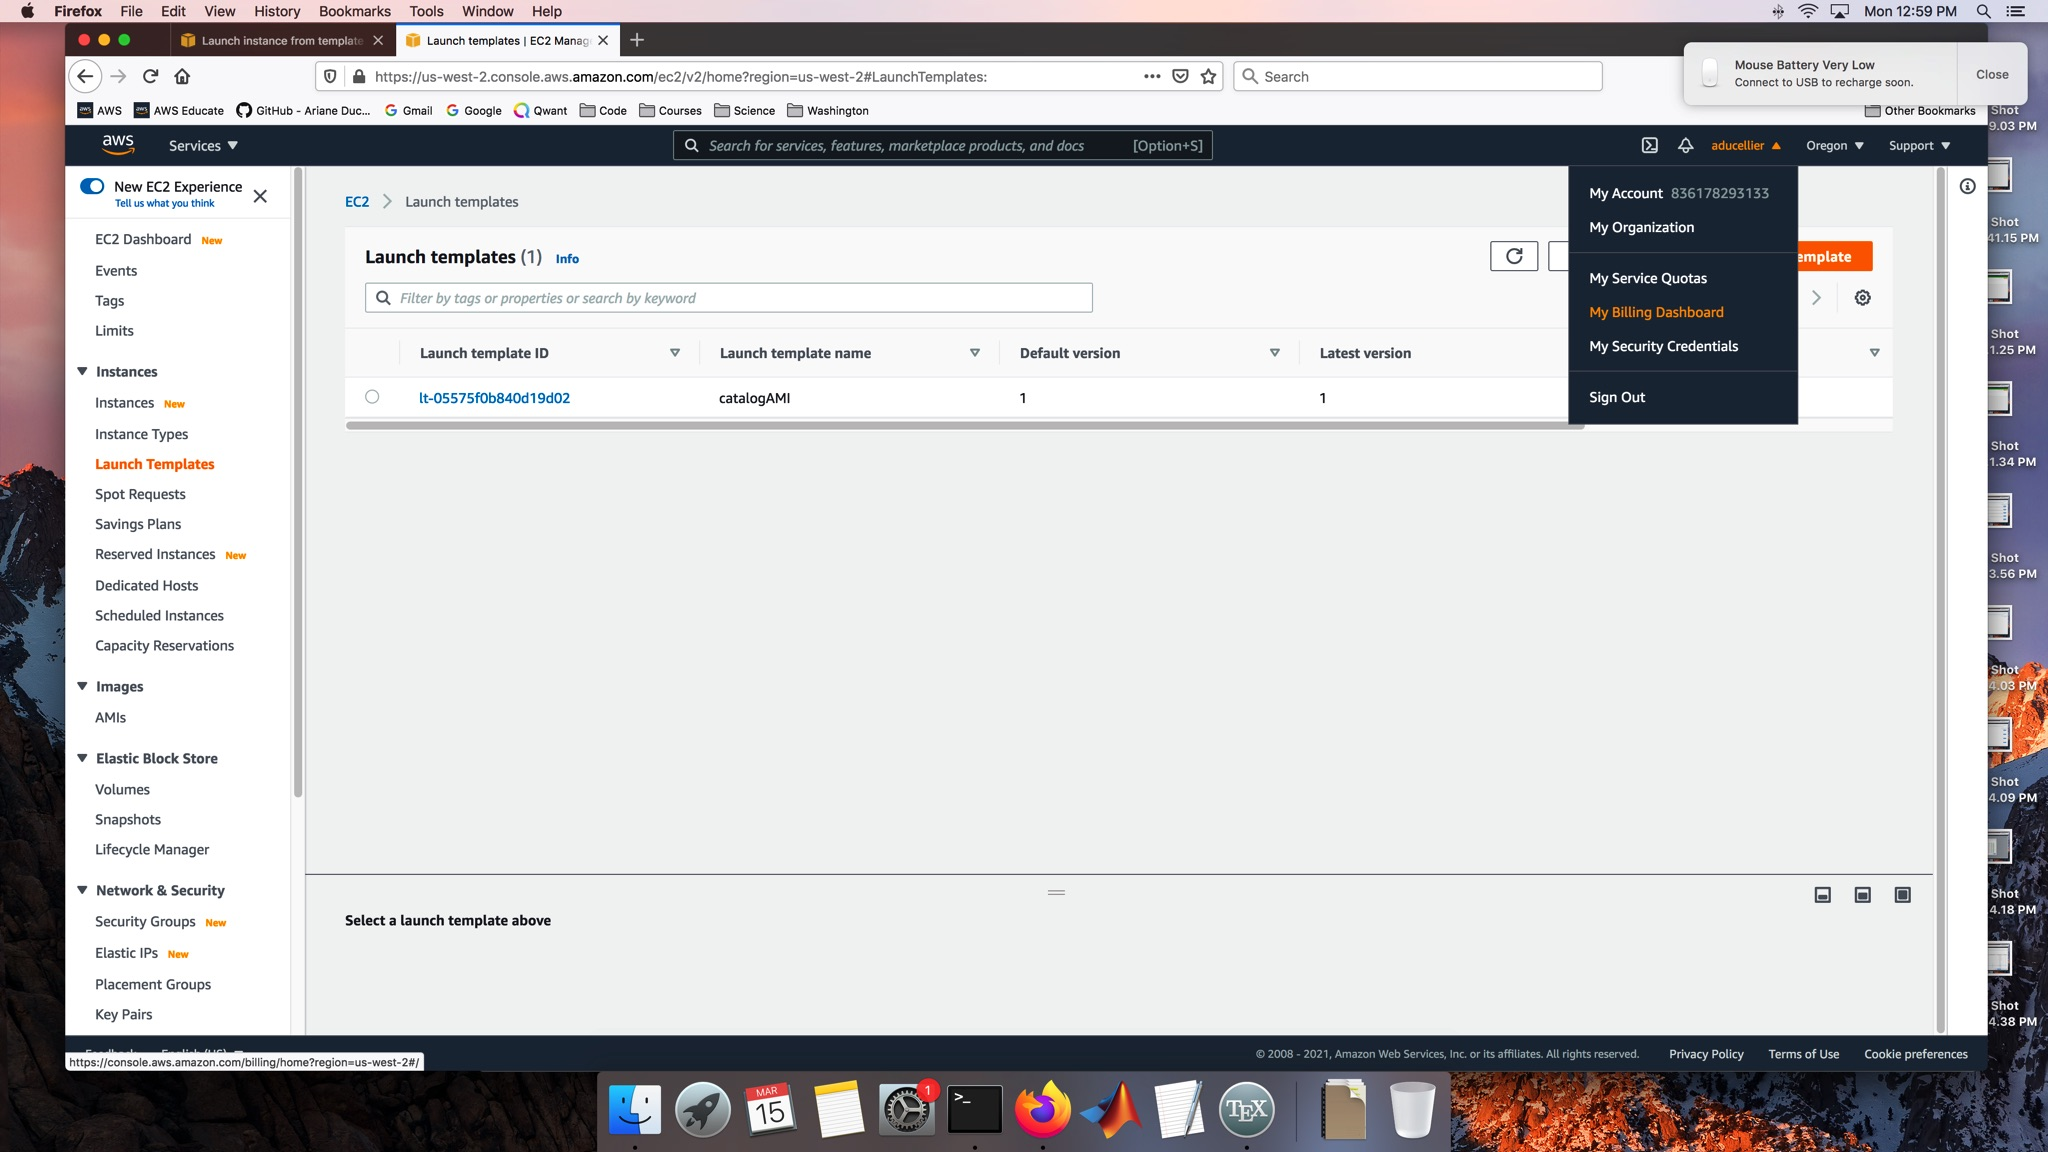
\includegraphics[width=11cm]{figures/billing_dashboard.jpg}};
		\draw<1>[red, thick] (8.5,4.4) rectangle ++(0.9,0.3);
	\end{tikzpicture}
	\end{frame}

	\begin{frame}
	\frametitle{You can check how much you have been spending (do it often!)}
	\begin{tikzpicture}
		\node[anchor=south west, inner sep=0] at (0,0) {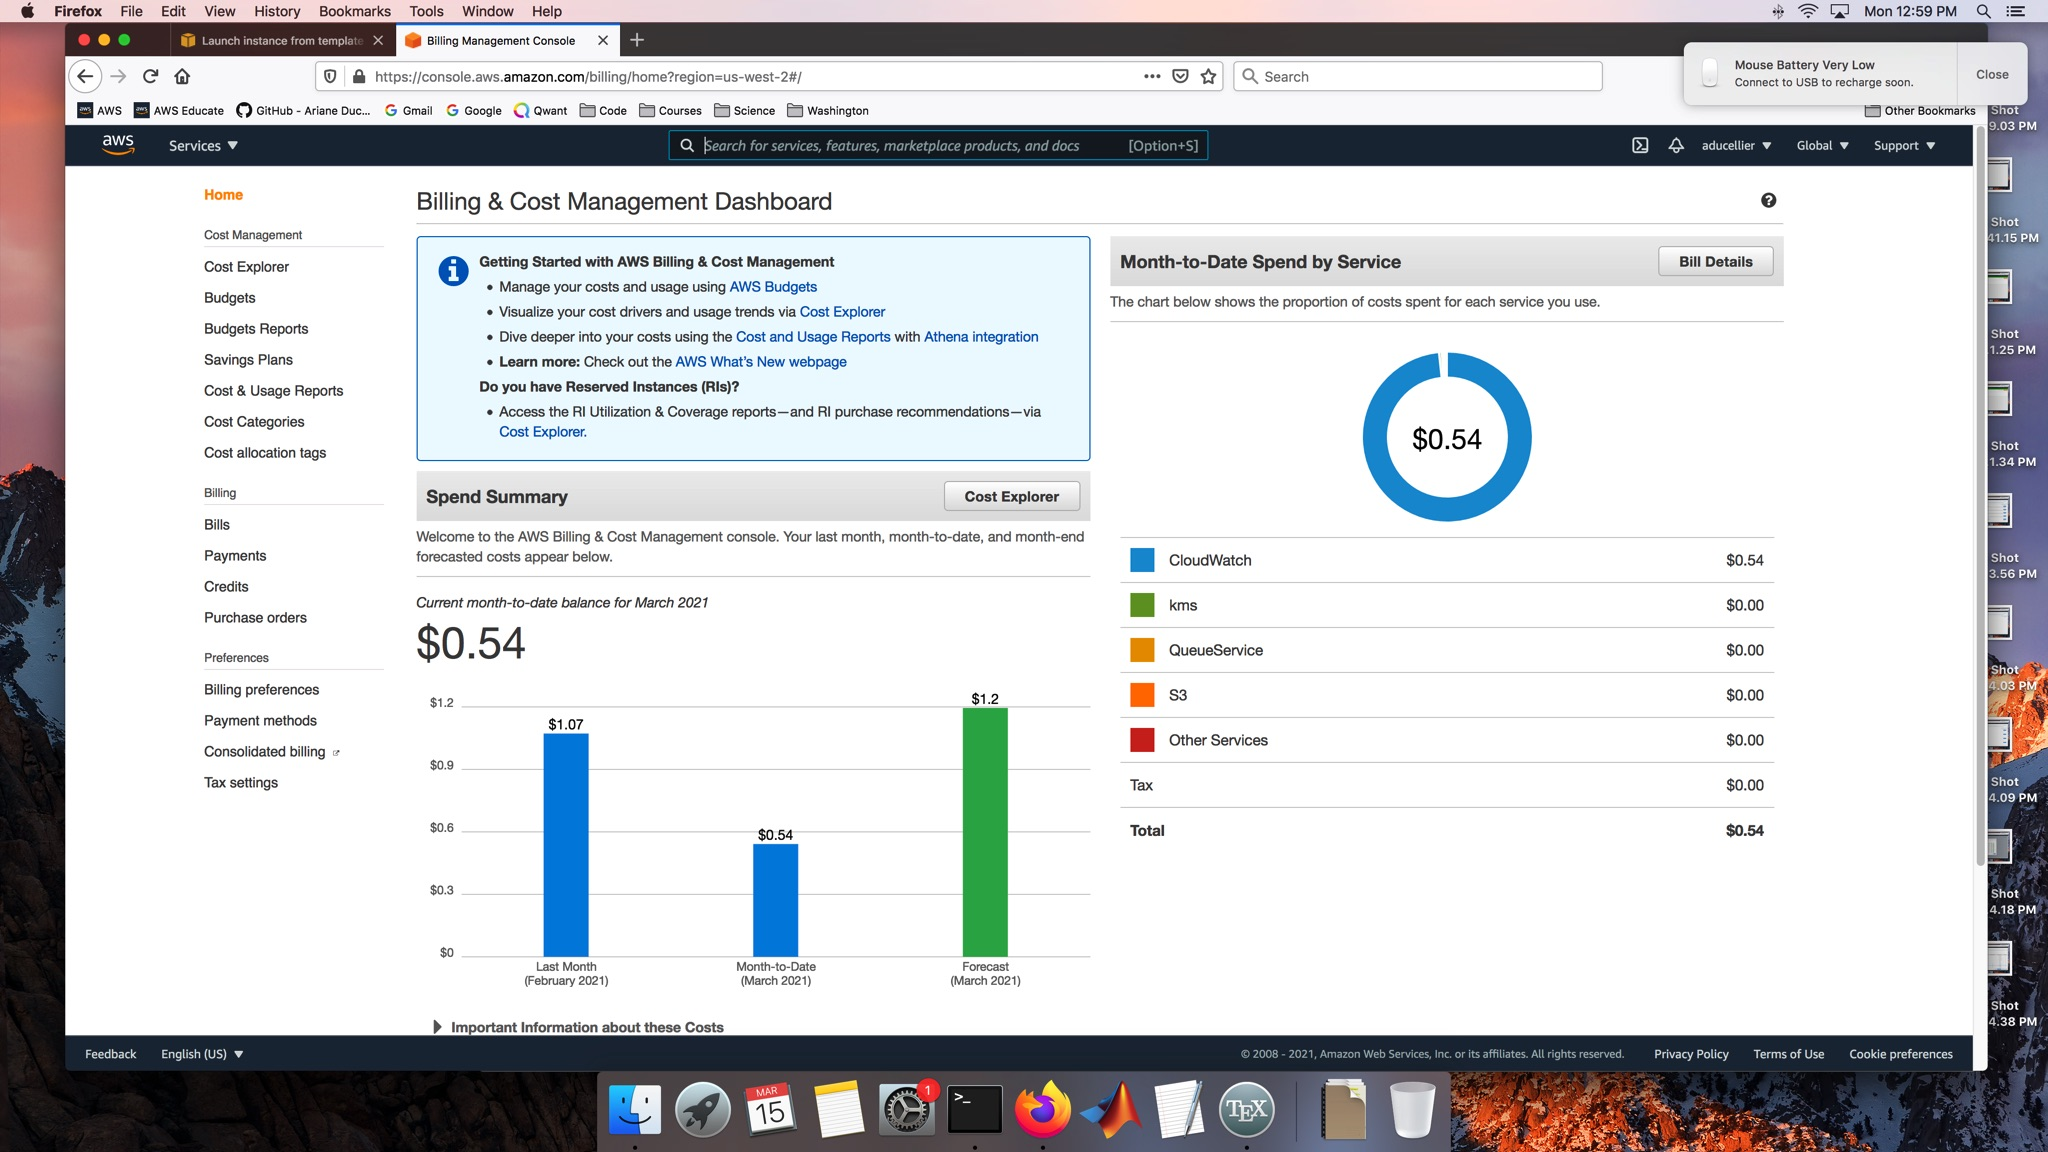
\includegraphics[width=11cm]{figures/billing_home.jpg}};
	\end{tikzpicture}
	\end{frame}

	\begin{frame}
	\frametitle{Go to \textit{Cost Explorer}}
	\begin{tikzpicture}
		\node[anchor=south west, inner sep=0] at (0,0) {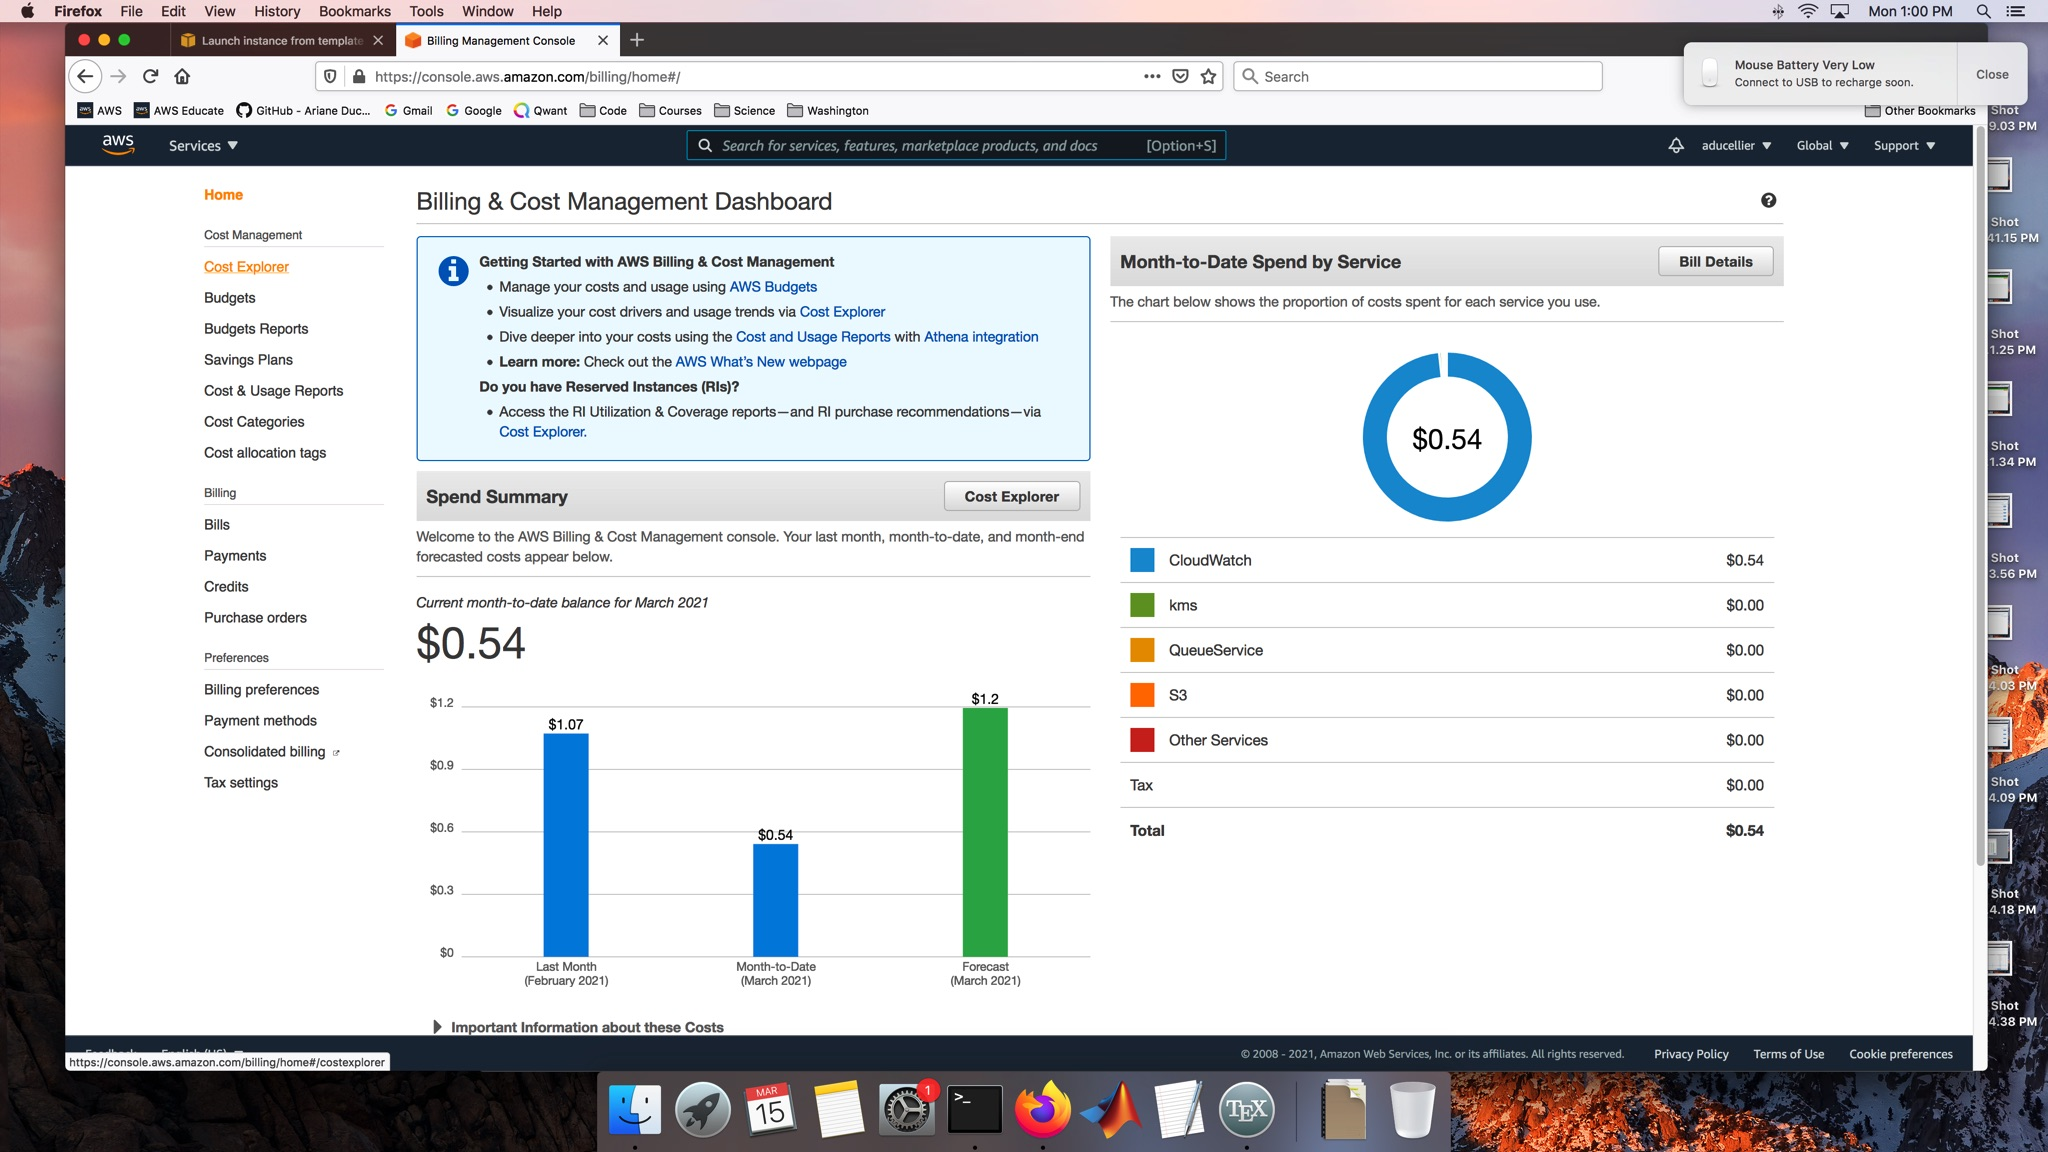
\includegraphics[width=11cm]{figures/go_to_cost_explorer.jpg}};
		\draw<1>[red, thick] (1.0,4.6) rectangle ++(0.6,0.3);
	\end{tikzpicture}
	\end{frame}

	\begin{frame}
	\frametitle{Look at the daily amounts you spent}
	\begin{tikzpicture}
		\node[anchor=south west, inner sep=0] at (0,0) {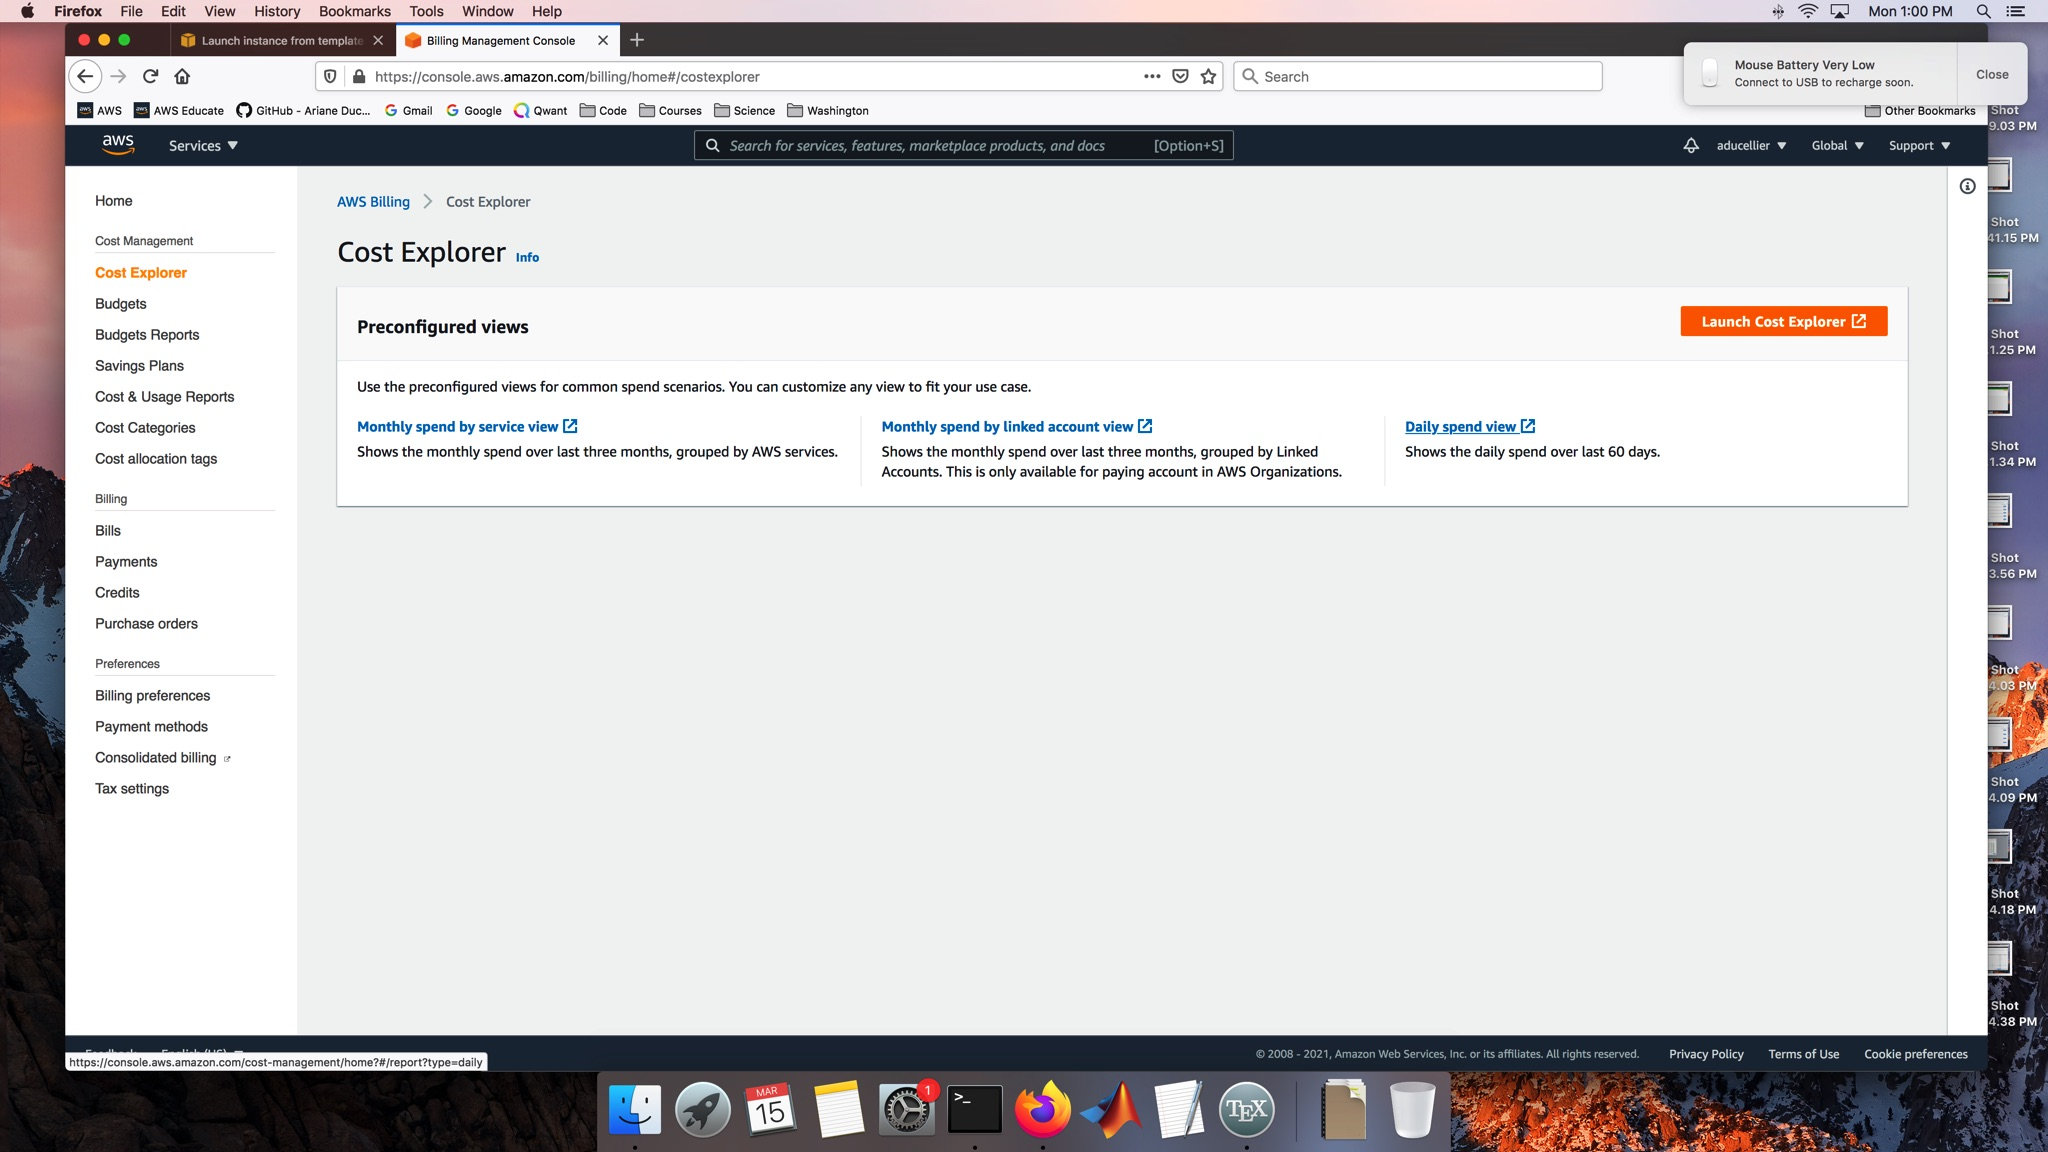
\includegraphics[width=11cm]{figures/daily_spend_view.jpg}};
		\draw<1>[red, thick] (7.5,3.6) rectangle ++(1.6,0.4);
	\end{tikzpicture}
	\end{frame}

	\begin{frame}
	\frametitle{Look at the daily amounts you spent}
	\begin{tikzpicture}
		\node[anchor=south west, inner sep=0] at (0,0) {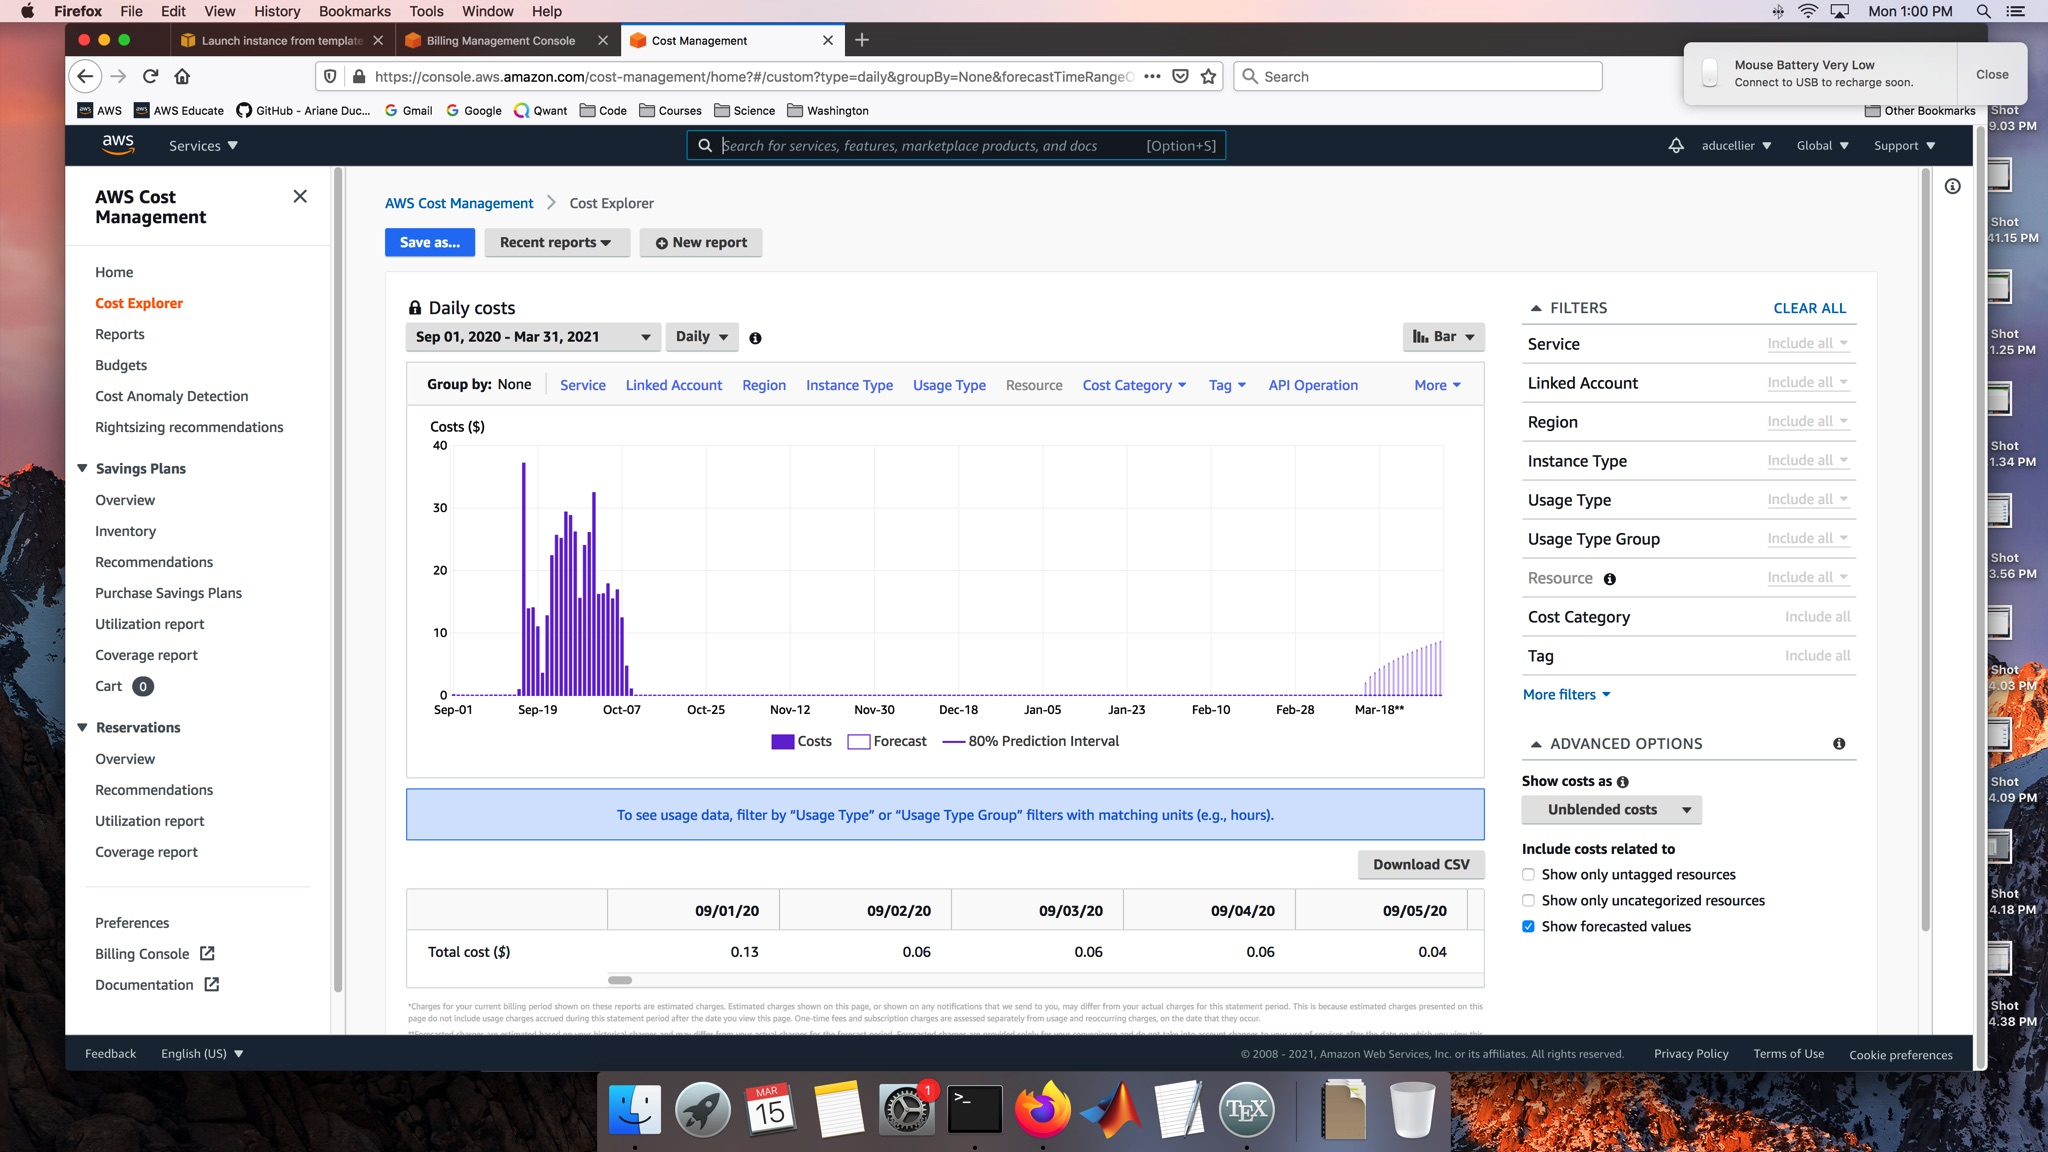
\includegraphics[width=11cm]{figures/see_history.jpg}};
	\end{tikzpicture}
	\end{frame}

	\begin{frame}
	\frametitle{Go to \textit{Budgets}}
	\begin{tikzpicture}
		\node[anchor=south west, inner sep=0] at (0,0) {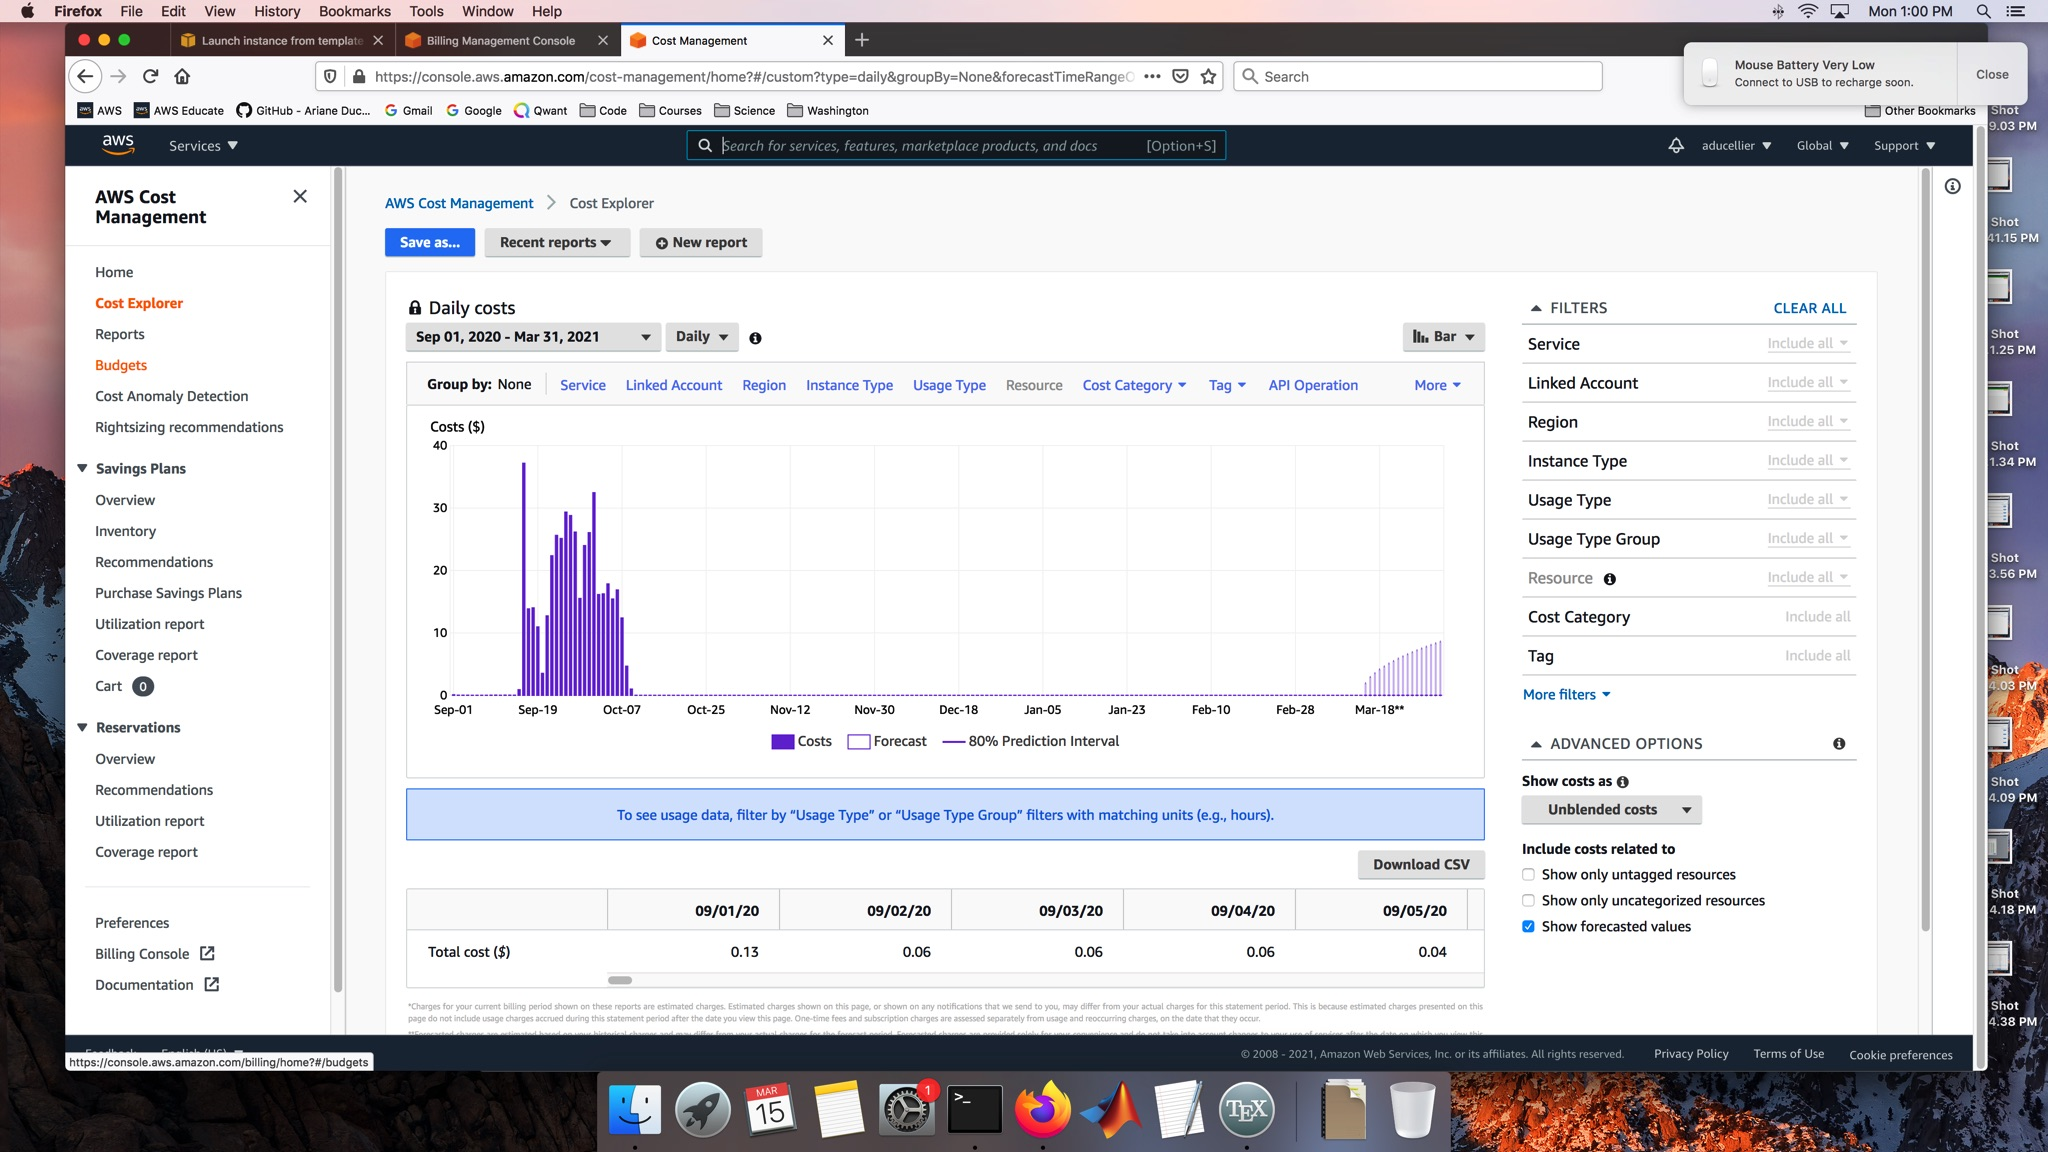
\includegraphics[width=11cm]{figures/go_to_budgets.jpg}};
		\draw<1>[red, thick] (0.5,4.1) rectangle ++(0.4,0.3);
	\end{tikzpicture}
	\end{frame}

	\begin{frame}
	\frametitle{You can create your own budgets}
	\begin{tikzpicture}
		\node[anchor=south west, inner sep=0] at (0,0) {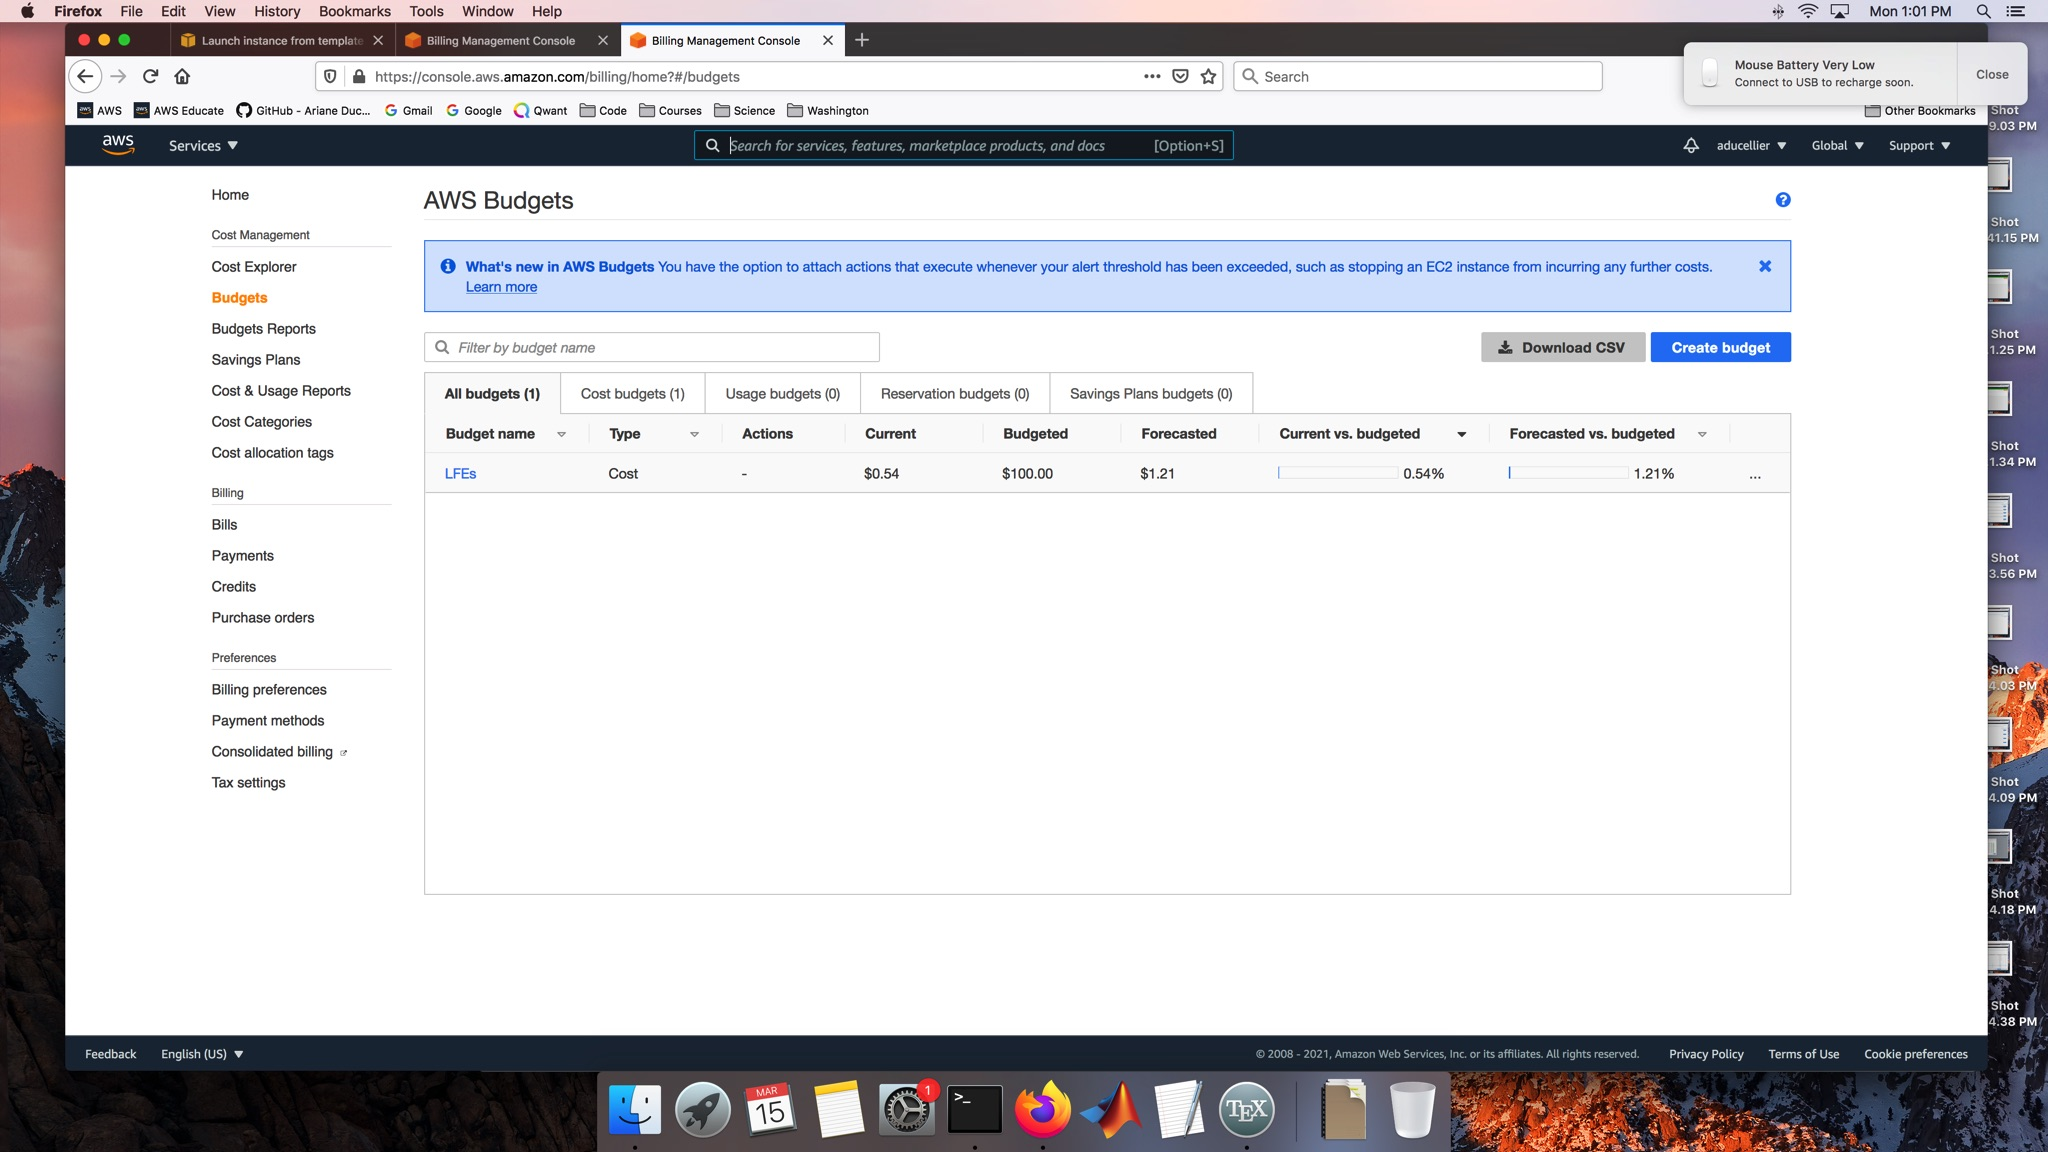
\includegraphics[width=11cm]{figures/create_budget.jpg}};
		\draw<1>[red, thick] (8.8,4.2) rectangle ++(0.9,0.3);
	\end{tikzpicture}
	\end{frame}

	\begin{frame}
	\frametitle{Some sources of funding}
	\begin{itemize}
		\item Become a member of the \href{https://depts.washington.edu/uwrcc/}{Research Computing Club} and apply for AWS credits through their \href{https://depts.washington.edu/uwrcc/getting-started-2/cloud-computing/}{Cloud Credit Program}.

		\vspace{0.5cm}

		\item Apply to the \href{https://environment.uw.edu/students/student-resources/scholarships-funding/graduate-scholarships-funding/other-graduate-funding-opportunities/integral-environmental-big-data-research-award/}{Integral Environmental Big Data Research Fund}: For graduate students, deadline in February.

		\vspace{0.5cm}

		\item Apply to an \href{https://www.microsoft.com/en-us/ai/ai-for-earth-grants}{Azure compute grant} if you want to use Azure instead of AWS, and your research focuses on Climate, Agriculture, Biodiversity, or Water.
	\end{itemize}
	\end{frame}

	\begin{frame}
	\frametitle{Workshop on Azure}
	\begin{itemize}
		\item Azure 101: Getting Started with Azure: \href{https://aka.ms/university-azure/GettingStartedAzure}{https://aka.ms/university-azure/GettingStartedAzure}
		\item Working with Data in Azure: \href{https://aka.ms/university-azure/DataOnAzure}{https://aka.ms/university-azure/DataOnAzure}
		\item Machine Learning on Azure: \href{https://aka.ms/university-azure/MachineLearning}{https://aka.ms/university-azure/MachineLearning}
		\item Office Hours: April 9 at 10am PST, April 16 at 10am PST, April 23 at 10am PST
	\end{itemize}
	\end{frame}

	\begin{frame}
	\frametitle{Most important points}
	\begin{itemize}
		\item Do not forget to terminate your instances.

		\vspace{0.5cm}

		\item Check your billing dashboard on a regular basis.

		\vspace{0.5cm}

		\item The EC2 dashboard shows only instances and keys for the region you have currently selected. Other instances may be running in other regions.
	\end{itemize}
	\end{frame}

	\begin{frame}
	\centering
		\Huge{Happy computing!}
	\end{frame}

%	\begin{frame}
%	Bonus: Create your own AMI
%	\end{frame}

\end{document}
